\documentclass{scrartcl}

\usepackage[utf8]{inputenc}
\usepackage[T1]{fontenc}
\usepackage{lmodern}
\usepackage{babel}
\usepackage{amsmath}
\usepackage{amsthm}
\usepackage{mathtools}
\usepackage[dvipsnames]{xcolor}
\usepackage{tikz}
\usepackage{pgfplots}
\usepackage{amssymb}
\usepackage{enumitem}
\usepackage{import}
\usepackage{subfigure}

\subimport{docs/libs/}{init}

\usetikzlibrary{patterns}
\usetikzlibrary{positioning}

\usepackage[
backend=biber,
% style=alphabetic,
sorting=none
]{biblatex}

\addbibresource{whitepaper.bib}

\title{Rule based Symbolic Reasoning}
\author{Matthias Lochbrunner}
\date{\today}

\theoremstyle{definition}
\newtheorem{exmp}{Example}[section]

\pgfplotsset{colormap/jet}

\tikzset{
    fromColorBar/.style={
        color of colormap={1000-#1*10},
        fill=.,
    },
}

\begin{document}
\maketitle
\begin{center}
	\textbf{Abstract}
\end{center}
\begin{abstract}
	% whats already there
	% They have to problem ...
	% my idea
	% promising results
    As computer algebra systems are used for decades, more and more machine learning approaches were published in recent years.
    They attempt to overcome the limitations of classical solvers by learning from data rather than hard-coding transformation rules.
    This splits the domain into two groups of programs, which exist side by side:
    Classical systems have been proven to be correct, but additional features require manual effort, and the new ones,
    which are able to discover new knowledge on their own, but the results can be incorrect.

    This paper proposes to address these issues by a rule-based reinforcement learning approach.
    The combination of a rule-based beam search and deep learning makes it possible to discover new knowledge without losing confidence in the correctness of the results.
    First prototypes provide promising results. 
	
	% The combination of a rule based beam search and deep learning is a promising approach to solve mathematical problems.
	% One obstacle to overcome is the amount of possible branches in this search as the number of applicable rules and the length of the calculation increases.
	% This paper proposes to address this issue by constantly shrinking the beam size with a multi-head neuronal network:
	% A policy head selects rules and positions in the current term.
	% A value head evaluates the probability that this calculation could lead to a desired solution.
	% Both heads help to reduce the beam size such that solving advanced mathematical problems becomes feasible.
\end{abstract}

\section{Motivation}

As current computer algebra systems use a complex but fixed set of rules to solve mathematical problems,
it takes manual effort to extend their capabilities \cite{wolfram}.
On the other hand, since 2020, more and more papers have been published describing how to solve mathematical problems using pure deep learning approaches.
They operate without any knowledge database, and their estimated solutions are subject to a certain degree of uncertainty.

Therefore Gary Marcus proposes a hybrid, knowledge-driven, reasoning-based approach centered around cognitive models,
that could provide the substrate for a richer, more robust AI than is currently possible. \cite{marcus2020decade}

This paper demonstrates one possible approach to do so:
A rule-based beam search guided by a reinforcement network setup.
The generic approach described here might be able to incorporate additional rules without requiring manual work.
Moreover, it is not limited to mathematical problems as long as a well-defined rule set can describe the domain.
The correctness of the result depends only on the correctness of the given ruleset.

\section{Related work}

The first outstanding paper was published by Lampe et al. in 2020.
They use state-of-the-art sequence to sequence transformers (Vaswani et al. \cite{vaswani2017attention}) on equations represented in the polish notation \cite{Lample2020Deep}.
This approach solves mathematical problems similar to translating a sentence from one language to another. 
% This approach views solving a mathematical problem as a translation problem.
% They don't use the concept of rules and tree structured data in the network.
Davis reviewed this work and came to the positive conclusion that their transformer model outperforms contemporary computer algebra systems.
However, he criticizes the limited vocabulary used in their generated data set \cite{davis2019use}.
In their latest paper, they widened the scope to five advanced mathematical problems and improved many of the limitations discussed by the community \cite{charton2021learning}.
Inspired by that work, Hahn et. al. also use a transformer based network for linear-time temporal logical formulas (LTL) \cite{hahn2021teaching}.
Similar to the result of the work by Lampe, their method is capable of solving large formulas.
Nevertheless, some of its predicted results are syntactically and semantically incorrect.

Lamb et al. presented a review on the relationship between GraphNeural Network (GNN) models and architectures and Neural-Symbolic Computing (NSC) \cite{lamb2020graph}.
They pointed out that this combination could provide trustful, explainable and robust AI systems.

Panju et al. build up a novel symbolic function learner to solve differential equations \cite{panju2020neurosymbolic}.
Their modeling approach is to iteratively feed the individual nodes of a syntax tree from the leaves to the root.
A very similar approach was elaborated by Piepenbrock et al. \cite{piepenbrock2021learning}. 
% This method is able to approximate a symbolic function when the problem has no elementary symbolic solution.

Rabe et al. worked out a significant improvement. They use an unsupervised proxy task to pre-train a sequence to sequence language model \cite{rabe2020mathematical}.
In their skip-tree training task, the model is trained to predict a subtree in the syntax tree of an expression.
It is remarkable that they consider typed inference for variables and propositional logic to some extent.

All of these approaches lack confidence in the correctness of the results as they simulate calculations.
They are not backed up by mechanisms that protect the algorithm from errors that lead to inaccurate results.

\section{Method}

The method I propose uses fundamental and well-known rules of the domain to overcome the drawbacks of existing methods.
% The method I propose is inspired by humans solving mathematical problems by hand.
% the  to overcame the drawbacks of existing methods. % todo
Given a problem, e.g. solve the equation $T_1\left(x\right)\equiv T_2\left(x\right)$ for $x$,
the beam search could try to apply various rules at different nodes in the syntax tree of the equation.
The policy head proposes the most promising combination of rules $R_j$ and positions $p_\ell$ in the current equation.
The value head evaluates the probability that the current step might lead to the desired solution.
The cumulative result of the value head can abort the attempt of a particular solution path, as it "seems" unlikely that this attempt would succeed \cite{44806}.

% Sub-section \ref{ssec:rule_application} will  
This section introduces the nomenclature and description of rule application to a given mathematical expression.
Followed by a presentation of a deep network architecture for tree-structured data.
The last part shows how to put the pieces together and set up a data loop.

\subsection{Rule Application}

A rule $R$ consists of one or multiple premises and one conclusion $B$.
In this paper we consider only rules that have a single premise $A$.
The outlook section discusses an approach with rules of multiple premisses. 
Every rule is then of the shape $A \Longrightarrow B$ or $A \equiv B$, which is equivalent to $A \Longleftrightarrow B$ or just the combination of $A \Longrightarrow B$ and $B \Longrightarrow A$.
Without loss of correctness we just use the first shape $A \Longrightarrow B$ in this paper.
Let's name the term $T$ with the depth $d$ of the corresponding syntax tree representation.

\begin{figure}[!htbp]
	\centering
	\subfigure[Index notation $p$]  
{
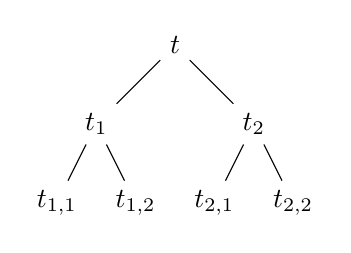
\begin{tikzpicture}
    \node (=) at (0,0){$t$};

    \node (+) at (-1,-1){$t_1$};
    \node (-) at (1,-1){$t_2$};
    \node (a) at (-1.5, -2) {$t_{1,1}$};
    \node (b) at (-0.5, -2) {$t_{1,2}$};
    \node (c) at (0.5, -2) {$t_{2,1}$};
    \node (d) at (1.5, -2) {$t_{2,2}$};

    \draw[] (=) -- (+);
    \draw[] (=) -- (-);
    \draw[] (+) -- (a);
    \draw[] (+) -- (b);
    \draw[] (-) -- (c);
    \draw[] (-) -- (d);
\end{tikzpicture}
}
\subfigure[Symbols $t_p$]  
{
\begin{tikzpicture}
    \node (=) at (0,0){$=$};
    \node (+) at (-1,-1){$+$};
    \node (-) at (1,-1){$-$};
    \node (a) at (-1.5, -2) {$a$};
    \node (b) at (-0.5, -2) {$b$};
    \node (c) at (0.5, -2) {$c$};
    \node (d) at (1.5, -2) {$d$};

    \draw[] (=) -- (+);
    \draw[] (=) -- (-);
    \draw[] (+) -- (a);
    \draw[] (+) -- (b);
    \draw[] (-) -- (c);
    \draw[] (-) -- (d);
\end{tikzpicture}
}
\subfigure[Sub-terms $T_p$]  
{
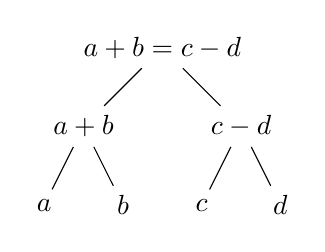
\begin{tikzpicture}
    \node (=) at (0,0){$a+b=c-d$};

    \node (+) at (-1,-1){$a+b$};
    \node (-) at (1,-1){$c-d$};
    \node (a) at (-1.5, -2) {$a$};
    \node (b) at (-0.5, -2) {$b$};
    \node (c) at (0.5, -2) {$c$};
    \node (d) at (1.5, -2) {$d$};

    \draw[] (=) -- (+);
    \draw[] (=) -- (-);
    \draw[] (+) -- (a);
    \draw[] (+) -- (b);
    \draw[] (-) -- (c);
    \draw[] (-) -- (d);
\end{tikzpicture}
}
\caption{
Example of the syntax tree for the term $a+b=c-d$ with $s=2$.
To demonstrate the usage of position variable $p$ consider sub-figure (b) the tree with the concrete symbols and sub-figure (a) the same tree with the abstract $t_p$ notation side by side.
% the concrete symbols (a) and the here used notation $t_p$.
For comparison the tree in sub-figure (c) contains the sub-terms $T_p$.
}
	\label{fig:sxntax_tree}
\end{figure}

As the term $T$ can be represented by a tree, we name it's child terms $T_p$ with the position $p \in \big\{\left( n_1, n_2, \dots, n_d \right) | n_i \in \mathbb{N}, n_i \leq s \big\}$.
Hence the sub-terms of $T$ are $T_p$.
For instance $T_1$ is the sub-term at the first child node of the root node in that tree and $T_{1,1}$ is the first child term of $T_1$ and so on.
The root symbol of $T_p$ should be $t_p$.
Figure \ref{fig:sxntax_tree} demonstrates this notation by an example term.
Let $s$ be the maximal number of children per node in the syntax tree.

We try to match the premise term $A_j$ of rule $R_j$ at any position $p$ in term $T$.
Doing so results in a set of possible positions $p_\ell$ with the required substitution table ${M_{j,\ell}: S_{A_j} \to S_{T_{p_\ell}}}$,
where $S_{T_{p_\ell}}$ is the set of the sub-terms in term $T_{p_\ell}$ and $S_{A_j}$ the set of free symbols in the premise $A_j$.
Free symbols are symbols not defined elsewhere such as standard operators or the number $\pi$ for instance.
Then the application of that rule results in the new terms $T^{(j,\ell)}$, where each sub-term at $p_\ell$ gets replaced by the substituted conclusion ${B_j'^{(\ell)} \coloneqq M_{j,\ell}\left( B_j \right)}$.
Where $B_j'^{(\ell)}$ is $B_j$ with symbols mapped back by $M_{j,\ell}$. 

\begin{exmp}
To illustrate the above, let's look at the application of the derivative rule for polynomials.

Consider the derivative rule
\begin{align}
	\frac{\partial}{\partial {\color{red}x}} {\color{red}x}^{\color{blue}n} \Longrightarrow {\color{blue}n}\cdot {\color{red}x}^{{\color{blue}n}-1} 
\end{align}
with the premise $A\equiv \frac{\partial}{\partial {\color{red}x}} {\color{red}x}^{\color{blue}n}$ and the conclusion $B\equiv {\color{blue}n}\cdot {\color{red}x}^{{\color{blue}n}-1}$.
This rule can be applied to the sub-term of
\begin{align}
	a = \frac{\partial}{\partial {\color{red}z}} {\color{red}z}^{\color{blue}4} + b
	\label{example:problem}
\end{align}
at position $p=\left(2,1\right)$ where the derivative $\frac{\partial}{\partial {\color{red}z}} {\color{red}z}^{\color{blue}4}$ is located.
Using the symbol mapping $M\left({\color{red}x}\right) = \color{red}z$ and $M\left({\color{blue}n} \right) = {\color{blue}4}$ leads to the substituted conclusion
\begin{align}
B' = M(B) = M({\color{blue}n}\cdot {\color{red}x}^{{\color{blue}n}-1}) = {M(\color{blue}n})\cdot M({\color{red}x})^{M({\color{blue}n})-1} = {\color{blue}4}\cdot {\color{red}z}^{{\color{blue}4}-1}
\end{align}.
Now you can replace the sub-term of equation (\ref{example:problem}) at position $p$ with with that $B'$ and you obtain the resulting new term
\begin{align}
	a = {\color{blue}4}\cdot {\color{red}z}^{{\color{blue}4}-1} + b
\end{align}.

\end{exmp}

\subsection{Indexed Convolution for Tree Structured Data}

Lampe et al. showed an approach where they unroll the term $T$ using the polish notation.
Then they apply contemporary NLP translation methods on that sequence, where the resulting "translated sentence" is the next step in the calculation \cite{Lample2020Deep}.
The approach discussed here keeps the tree structure.
It turned out that a Tree-LSTM network performs poorly on that data \cite{tai2015improved}.

This paper will discuss the adoption of a network architecture using indexed convolution operations.
An attention-based network with particular positional encoding is discussed in the outlook. 
The indexed CNN operation performs a convolution of each node, with its neighbor nodes and itself.
Figure \ref{fig:index_tensor} demonstrates the operation by a simple example.

\begin{figure}[!htbp]
	\centering
	
    \tikzset{
        hatch distance/.store in=\hatchdistance,
        hatch distance=24pt,
        hatch thickness/.store in=\hatchthickness,
        hatch thickness=8pt
    }
\makeatletter
\pgfdeclarepatternformonly[\hatchdistance,\hatchthickness]{flexible hatch}
{\pgfqpoint{0pt}{0pt}}
{\pgfqpoint{\hatchdistance}{\hatchdistance}}
{\pgfpoint{\hatchdistance-1pt}{\hatchdistance-1pt}}%
{
    \pgfsetcolor{\tikz@pattern@color}
    \pgfsetlinewidth{\hatchthickness}
    \pgfpathmoveto{\pgfqpoint{0pt}{0pt}}
    \pgfpathlineto{\pgfqpoint{\hatchdistance}{\hatchdistance}}
    \pgfusepath{stroke}
}
\makeatother

\subfigure[Neighbors of the root.
$\scriptstyle \phi'_=={\color{red}w_1\phi_=}+{\color{blue}w_2\phi_+}+{\color{green!70!black}w_3\phi_-}+{\color{orange!80!black}w_4\phi_{\text{PAD}}}$]  
{
\tikzset{g_style/.style={black, draw=black!15, minimum size=0.5cm}}
\begin{tikzpicture}
    \node[g_style,fill=red!20,draw=black] (=) at (0,0){=};
    \node[g_style,fill=blue!20] (+) at (-1,-1){$+$};
    \node[g_style,fill=green!20] (-) at (1,-1){$-$};
    \node[g_style] (a) at (-1.5, -2) {$a$};
    \node[g_style] (b) at (-0.5, -2) {$b$};
    \node[g_style] (c) at (0.5, -2) {$c$};
    \node[g_style] (d) at (1.5, -2) {$d$};
    \node[g_style,fill=orange!20] at (1.5, 0) {\tiny PAD};

    \draw[draw=blue!70] (=) -- (+);
    \draw[draw=green!70] (=) -- (-);
    \draw[] (+) -- (a);
    \draw[] (+) -- (b);
    \draw[] (-) -- (c);
    \draw[] (-) -- (d);
\end{tikzpicture}
}
\subfigure[Neighbors of a left node $+$
$\scriptstyle \phi'_+={\color{red}w_1\phi_+}+{\color{blue}w_2\phi_a}+{\color{green!70!black}w_3\phi_b}+{\color{orange!80!black}w_4\phi_=}$]  
{
\tikzset{g_style/.style={black, draw=black!15, minimum size=0.5cm}}
\begin{tikzpicture}
    \node[g_style,fill=orange!20] (=) at (0,0){=};
    \node[g_style,fill=red!20,draw=black] (+) at (-1,-1){$+$};
    \node[g_style] (-) at (1,-1){$-$};
    \node[g_style,fill=blue!20] (a) at (-1.5, -2) {$a$};
    \node[g_style,fill=green!20] (b) at (-0.5, -2) {$b$};
    \node[g_style] (c) at (0.5, -2) {$c$};
    \node[g_style] (d) at (1.5, -2) {$d$};
    \node[g_style] at (1.5, 0) {\tiny PAD};

    \draw[draw=orange!70] (=) -- (+);
    \draw[] (=) -- (-);
    \draw[draw=blue!70] (+) -- (a);
    \draw[draw=green!70] (+) -- (b);
    \draw[] (-) -- (c);
    \draw[] (-) -- (d);
\end{tikzpicture}
}
\subfigure[Neighbors of a leaf $b$
$\scriptstyle \phi'_b={\color{red}w_1\phi_b}+{\color{blue}w_2\phi_{\text{PAD}}}+{\color{green!70!black}w_3\phi_{\text{PAD}}}+{\color{orange!80!black}w_4\phi_+}$]  
{
\tikzset{g_style/.style={black, draw=black!15, minimum size=0.5cm}}
\begin{tikzpicture}
    \node[g_style] (=) at (0,0){=};
    \node[g_style,fill=orange!20] (+) at (-1,-1){$+$};
    \node[g_style] (-) at (1,-1){$-$};
    \node[g_style] (a) at (-1.5, -2) {$a$};
    \node[g_style,fill=red!20,draw=black] (b) at (-0.5, -2) {$b$};
    \node[g_style] (c) at (0.5, -2) {$c$};
    \node[g_style] (d) at (1.5, -2) {$d$};
    {
        \node[preaction={fill=blue!20}, g_style, pattern=flexible hatch, pattern color=green!20] at (1.5, 0) {\tiny PAD};
    }

    \draw[] (=) -- (+);
    \draw[] (=) -- (-);
    \draw[] (+) -- (a);
    \draw[draw=orange!70] (+) -- (b);
    \draw[] (-) -- (c);
    \draw[] (-) -- (d);
\end{tikzpicture}
}
\caption{
    Example of indexed convolution operation on term $a+b=c+d$.
    Sub-figure (b) shows the computation of the next value $\phi' = C\left(\phi\right)$ for the node $a$ in that term.
    It is the weighted sum of the current values of itself, it's children and the parent.
    As the root in (a) has no parent node, we use the padding as a default node.
    The same is true for the child-nodes of a leaf in sub-figure (c).
    The colors red (self), blue (first child), green (second child) and orange (parent) indicated the neighbors of the focused node in each sub-plot.
}
	\label{fig:index_tensor}
\end{figure}

In order to increase the computing efficiency, each term gets unrolled.
The unrolled term $T$ with $s=2$ using breadth-first is the vector $\left( t, t_1, t_2, t_{1,1},t_{1,2}, t_{2,1}, t_{2,2}, \cdots \right) \equiv  \left( t_{p_1}, t_{p_2}, t_{p_3},\cdots, t_{p_L} \right)$ of length $L$.
Hence in index notation $t_{p_\ell}$ with $\ell \in \left\{1., \cdots,L\right\}$ is the index of symbol $t_p$ in the unrolled term.
An index map $g \in \mathbb{N}^{L\times \left(K\right)}$ carries the indices of the neighbors in a fixed order.
The kernel $K= s+2$ depends on the maximal spread of all terms in a batch.
The index map of example in figure \ref{fig:index_tensor} would look like

\begin{align}
	g_{\ell,k} = 
	\begin{pmatrix}
		1 & 2 & 3 & 4 & 5 & 6 & 7 \\
		2 & 4 & 6 & 0 & 0 & 0 & 0 \\
		3 & 5 & 7 & 0 & 0 & 0 & 0 \\
		0 & 1 & 1 & 2 & 2 & 3 & 3 \\
	\end{pmatrix}^\top
\end{align}

where index $0$ points to the padding.


\begin{figure}[!htbp]
	\centering
	\def\ConvColor{rgb:yellow,5;red,2.5;white,5}
\def\ConvReluColor{rgb:yellow,5;red,5;white,5}

% keine batch
\begin{tikzpicture}
\tikzstyle{connection}=[ultra thick,every node/.style={sloped,allow upside down},draw=\edgecolor,opacity=0.7]

\pic[shift={(0,0,0)}] at (0,0,0) {RightBandedBox={name=ix,caption=x,%
        xlabel={{"t", "f"}},ylabel=L,zlabel=b,fill=\ConvColor,bandfill=\ConvColor,%
        height=8,width={2, 3},depth=8}};

\pic[shift={(0,3,0)}] at (0,0,0) {Box={name=i1,caption=g,%
        xlabel={{"2+s"}},ylabel=L,zlabel=b,fill=\ConvColor,%
        height=8,width={2},depth=8}};

\pic[shift={(2,0,0)}] at (ix-east) {RightBandedBox={name=ic1,caption=iconv,%
        xlabel={{"e"}},ylabel=L,zlabel=b,fill=\ConvColor,bandfill=\ConvReluColor,%
        height=10,width={3},depth=10}};

\pic[shift={(4,0,0)}] at (ix-east) {RightBandedBox={name=ic2,caption=iconv,%
        xlabel={{"e"}},ylabel=L,zlabel=b,fill=\ConvColor,bandfill=\ConvReluColor,%
        height=10,width={3},depth=10}};

% heads

\pic[shift={(8,0,-4)}] at (ix-east) {RightBandedBox={name=icv,caption=iconv,%
xlabel={{"e"}},ylabel=L,zlabel=b,fill=\ConvColor,bandfill=\ConvReluColor,%
height=10,width={3},depth=10}};

\pic[shift={(10,0,-4)}] at (ix-east) {Box={name=ov,caption=value,%
xlabel={{"1"}},zlabel=b,ylabel=1,fill=\ConvColor,%
height=1,width={1},depth=10}};

\pic[shift={(8,0,4)}] at (ix-east) {RightBandedBox={name=icp,caption=iconv,%
        xlabel={{"e", "dummy"}},ylabel=L,zlabel=b,fill=\ConvColor,bandfill=\ConvReluColor,%
        height=10,width={3},depth=10}};

\pic[shift={(10,0,4)}] at (ix-east) {Box={name=op,caption=policy,%
        xlabel={{"r", "dummy"}},ylabel=L,zlabel=b,fill=\ConvColor,%
        height=10,width={8},depth=10}};


\path (ix-east) -- (ix-west) coordinate[pos=0.4] (after4) ;

\draw [connection] (ix-east) -- node {\midarrow} (ic1-west);
\draw [connection]  (ic1-east) -- node {\midarrow} (ic2-west);
\draw [connection]  (ic2-east) -- node {\midarrow} (icv-west);
\draw [connection]  (icv-east) -- node {\midarrow} (ov-west);
\draw [connection]  (ic2-east) -- node {\midarrow} (icp-west);
\draw [connection]  (icp-east) -- node {\midarrow} (op-west);

\draw [connection] (i1-east) -- ++ (2.5,0,0) -- node {\midarrow} (ic1-west);
\draw [connection] (i1-east) -- ++ (4.5,0,0) -- node {\midarrow} (ic2-west);
\draw [connection] (i1-east) -- ++ (5,0,0) -- ++ (3.5, 0, -4) -- node {\midarrow} (icv-west);
\draw [connection] (i1-east) -- ++ (5,0,0) -- ++ (3.5, 0, +4) -- node {\midarrow} (icp-west);

\end{tikzpicture}

	\caption{While $x\in \mathbb{R}^{L\times E}$ is the input tensor with $E=t+f$ encoded features per symbol $t_\ell$, the network needs the index tensor $g$ is an additional input.
		While $t$ is the encoding of the symbol's word representation and $f$ contains some additional properties of that symbol.
		Each indexed convolution operation (iconv) reads from that index tensor.
		The policy head returns a matrix with the axis rule id $j$ and path id $\ell$. 
		The output of the value head is just a scalar. 
	}
	\label{fig:iconv_network}
\end{figure}

Convolving over the input $x \in \mathbb{R}^{L\times I}$ with indexed convolution $C$, input channel $i \in \left\{1,\cdots,I \right\}$,
the kernel weights $w \in \mathbb{R}^{\left( s+2 \right)\times I \times J}$, output channel $j \in \left\{1,\cdots,J\right\}$ and bias $b \in \mathbb{R}^J$,
is defined as

\begin{align}
	C\left( x, g, w, b \right)_{\ell j} \coloneqq \sum_{ki}x_{g_{\ell k}i} w_{kij}+b_j
\end{align}

Figure \ref{fig:iconv_network} shows an overview of the multi-head network architecture, where the index tensor $g_{\ell k}$ gets distributed to each indexed convolution layer.
These layers are used in the backbone and in the heads.
Due to the padding and stride of one, the indexed convolution retains the shape of the input tensor, except for the configurable channel size.
Therefore this operation is appropriate for stacking deep networks.
A deeper network leads to a larger receptive field and considers more distant symbols.

This is useful for the policy head, assigning each sub-term a possibility estimation of the most promising rules to apply.

\begin{figure}[!htbp]
	\centering
	
% sample id: #19818
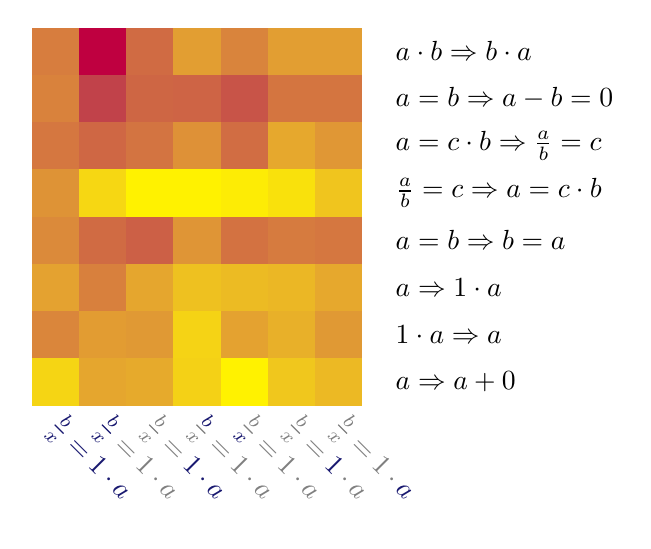
\begin{tikzpicture}[scale=0.6]
    \foreach \y [count=\p] in {
        {40,0,30,58,44,58,58},
        {43,6,27,26,17,36,36},
        {37,28,35,51,31,63,54},
        {52,87,100,100,97,92,78},
        {47,30,24,53,34,39,37},
        {60,42,62,76,73,71,63},
        {45,57,55,85,60,67,55},
        {86,62,64,84,100,79,72},
        } {
        \foreach \x [count=\r] in \y {
            \node[fill=yellow!\x!purple, minimum size=6mm, text=white] at (\r,-\p) {};
        }
    }
    \foreach \t [count=\p] in {
        $a\cdot b \Rightarrow b\cdot a $,
        $a=b \Rightarrow a-b=0 $,
        $a=c\cdot b \Rightarrow \frac{a}{b}=c $,
        $\frac{a}{b}=c \Rightarrow a=c\cdot b $,
        $a=b \Rightarrow b=a $,
        $a \Rightarrow 1\cdot a $,
        $1\cdot a \Rightarrow a $,
        $a \Rightarrow a+0 $
    } {
        \node[anchor=west] at (8, -\p) {\t};
    }
    \foreach \t [count=\r] in {
        $\textcolor{MidnightBlue}{\frac{b}{x}=1\cdot a}$,
        $\textcolor{Gray}{\textcolor{MidnightBlue}{\frac{b}{x}}=1\cdot a}$,
        $\textcolor{Gray}{\frac{b}{x}=\textcolor{MidnightBlue}{1\cdot a}}$,
        $\textcolor{Gray}{\frac{\textcolor{MidnightBlue}{b}}{x}=1\cdot a}$,
        $\textcolor{Gray}{\frac{b}{\textcolor{MidnightBlue}{x}}=1\cdot a}$,
        $\textcolor{Gray}{\frac{b}{x}=\textcolor{MidnightBlue}{1}\cdot a}$,
        $\textcolor{Gray}{\frac{b}{x}=1\cdot \textcolor{MidnightBlue}{a}}$
    } {
        \node[anchor=west, rotate=-45] at (\r - 0.2, -8.7) {\t};
    }
    \end{tikzpicture}
    
	\caption{Policy Network output normed to the range $[0,100]$: Each row is a possible rule $R_j$. Each column a sub-term $T_{p_\ell}$ of the initial term $T$ (highlighted in blue font).
	Rules which are not applicable to any $T_{p_\ell}$ are not shown here.
	}
	\label{fig:network_output}
\end{figure}

Figure \ref{fig:network_output} demonstrates the output of the policy head applied on the term $\frac{b}{x}=1\cdot a$.
% Find better example
This heat-map shows that dividing the equation by $a$ is more promising than blowing it up with the rules in the lower part of the map.
% The value head estimates the probability that the input term can lead to a solution.


\subsection{Three-T-Loop}

The training set consists of problems generated with the computer algebra system Sympy \cite{10.7717/peerj-cs.103}.
A training sample has a rule like shape $T^\text{Initial} \Longrightarrow T^\text{Target}$ where $T^\text{Initial}$ is the initial problem term and $T^\text{Target}$ the solution or target term.
The goal is to find the shortest chain of rule applications from $T^\text{Initial}$ to $T^\text{Target}$:

\begin{align}
	T^\text{Initial} \Longrightarrow T^{(j_1)} \Longrightarrow T^{(j_1j_2)} \Longrightarrow \cdots \Longrightarrow T^\text{Target}
	\label{eq:calculation_chain}
\end{align}

To obtain training data from the given problem set, we use an initial beam search without the assistance of a network.
This can already solve a few simple problems, and training data can be extracted from these solution paths.
% Let's call this procedure \textit{three-T-loop} which consists of these three steps:
In order to solve more complex problems we choose an iterative approach.
The so called \textit{three-T-loop}.
The data loop consists of three steps:

% how is the network output used

\begin{enumerate}[label=(\roman*)]
	\item \textbf{Try} to solve some of the training problems.
	\item \textbf{Trace} the calculation steps of the solved problems and create training data out of them. 
	\item \textbf{Train} the model with the training data from the previous step.
\end{enumerate}

In each iteration of this \textit{three-T-loop} we gain more training data.
% As the network's performance increases, it can solve more and more problems.
With more training data, the network performance increases, and it can solve more problems.
The trained network also reduces the number of misleading rule applications.
The value head helps to decide whether the calculation path seems promising to achieve a suitable result.
If the accumulated values are below a threshold the current path gets aborted to save resources (see Figure \ref{fig:beam_search} on page \pageref{fig:beam_search}). 

In order to get the model not making the same mistakes over and over again, it is crucial to add samples of calculations that did not lead to a solution to the training data. 
These negative samples are present in the training set for value and policy head.


The \textit{three-T-loop} can be extended by a fourth step discussed in the outlook section, which allows incorporating useful sub-chains of formula (\ref{eq:calculation_chain}) into the ruleset.

\begin{figure}[!htbp]
	\centering
	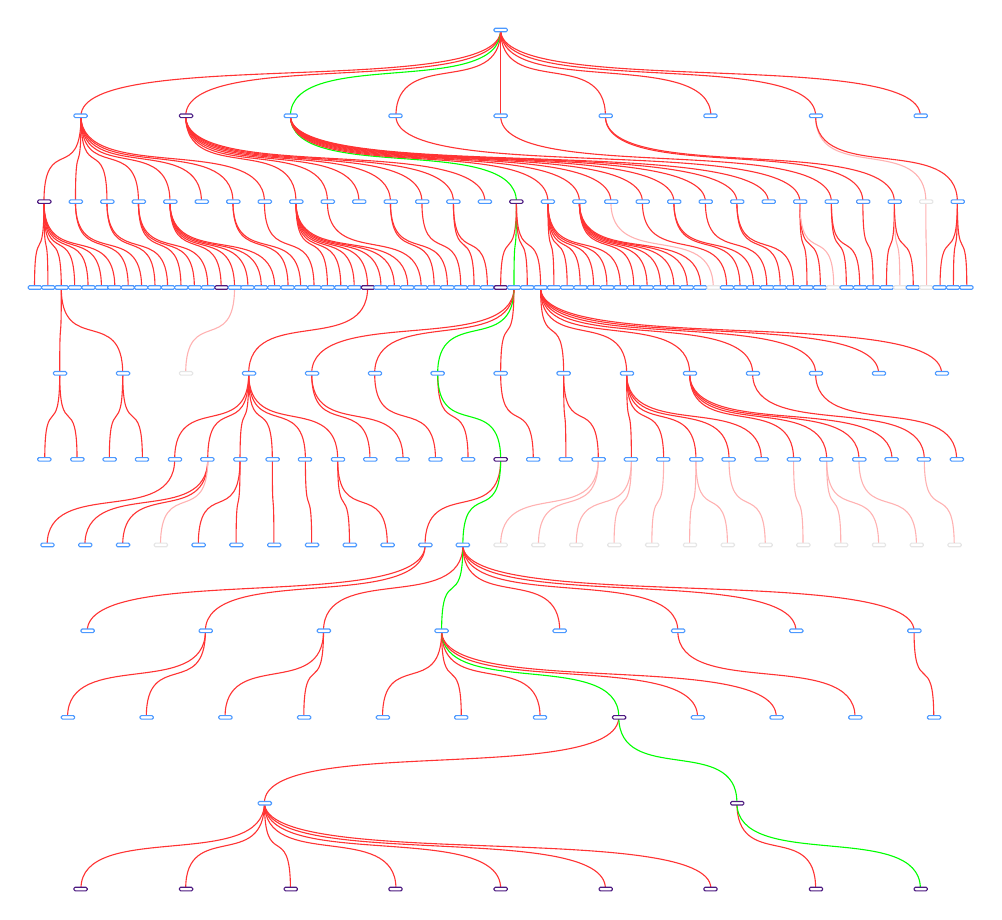
\begin{tikzpicture}[every node/.style={rectangle,fill=white,rounded corners=0.451}]
	\tikzset{xcolor/.code args={#1=#2}{
		\definecolor{mytemp}{rgb}{#2}
		\tikzset{draw=mytemp}
		}
	}
	\fontsize{0.5634}{0.6761}\selectfont
	\draw[draw=red!80] (-5.33,4.36) .. controls (-5.33,5.24) and (0.00,4.58) .. (0.00,5.45);
	\draw[draw=red!80] (-5.80,3.27) .. controls (-5.80,4.15) and (-5.33,3.49) .. (-5.33,4.36);
	\draw[draw=red!80] (-5.92,2.18) .. controls (-5.92,3.05) and (-5.80,2.40) .. (-5.80,3.27);
	\draw[draw=red!80] (-5.75,2.18) .. controls (-5.75,3.05) and (-5.80,2.40) .. (-5.80,3.27);
	\draw[draw=red!80] (-5.58,2.18) .. controls (-5.58,3.05) and (-5.80,2.40) .. (-5.80,3.27);
	\draw[draw=red!80] (-5.60,1.09) .. controls (-5.60,1.96) and (-5.58,1.31) .. (-5.58,2.18);
	\draw[draw=red!80] (-5.79,-8.88e-16) .. controls (-5.79,0.873) and (-5.60,0.218) .. (-5.60,1.09);
	\draw[draw=red!80] (-5.38,-8.88e-16) .. controls (-5.38,0.873) and (-5.60,0.218) .. (-5.60,1.09);
	\draw[draw=red!80] (-4.80,1.09) .. controls (-4.80,1.96) and (-5.58,1.31) .. (-5.58,2.18);
	\draw[draw=red!80] (-4.97,-8.88e-16) .. controls (-4.97,0.873) and (-4.80,0.218) .. (-4.80,1.09);
	\draw[draw=red!80] (-4.55,-8.88e-16) .. controls (-4.55,0.873) and (-4.80,0.218) .. (-4.80,1.09);
	\draw[draw=red!80] (-5.41,2.18) .. controls (-5.41,3.05) and (-5.80,2.40) .. (-5.80,3.27);
	\draw[draw=red!80] (-5.24,2.18) .. controls (-5.24,3.05) and (-5.80,2.40) .. (-5.80,3.27);
	\draw[draw=red!80] (-5.07,2.18) .. controls (-5.07,3.05) and (-5.80,2.40) .. (-5.80,3.27);
	\draw[draw=red!80] (-4.90,2.18) .. controls (-4.90,3.05) and (-5.80,2.40) .. (-5.80,3.27);
	\draw[draw=red!80] (-5.40,3.27) .. controls (-5.40,4.15) and (-5.33,3.49) .. (-5.33,4.36);
	\draw[draw=red!80] (-4.73,2.18) .. controls (-4.73,3.05) and (-5.40,2.40) .. (-5.40,3.27);
	\draw[draw=red!80] (-4.56,2.18) .. controls (-4.56,3.05) and (-5.40,2.40) .. (-5.40,3.27);
	\draw[draw=red!80] (-5.00,3.27) .. controls (-5.00,4.15) and (-5.33,3.49) .. (-5.33,4.36);
	\draw[draw=red!80] (-4.39,2.18) .. controls (-4.39,3.05) and (-5.00,2.40) .. (-5.00,3.27);
	\draw[draw=red!80] (-4.23,2.18) .. controls (-4.23,3.05) and (-5.00,2.40) .. (-5.00,3.27);
	\draw[draw=red!80] (-4.60,3.27) .. controls (-4.60,4.15) and (-5.33,3.49) .. (-5.33,4.36);
	\draw[draw=red!80] (-4.06,2.18) .. controls (-4.06,3.05) and (-4.60,2.40) .. (-4.60,3.27);
	\draw[draw=red!80] (-3.89,2.18) .. controls (-3.89,3.05) and (-4.60,2.40) .. (-4.60,3.27);
	\draw[draw=red!80] (-3.72,2.18) .. controls (-3.72,3.05) and (-4.60,2.40) .. (-4.60,3.27);
	\draw[draw=red!80] (-4.20,3.27) .. controls (-4.20,4.15) and (-5.33,3.49) .. (-5.33,4.36);
	\draw[draw=red!80] (-3.55,2.18) .. controls (-3.55,3.05) and (-4.20,2.40) .. (-4.20,3.27);
	\draw[draw=red!80] (-3.38,2.18) .. controls (-3.38,3.05) and (-4.20,2.40) .. (-4.20,3.27);
	\draw[draw=red!30] (-4.00,1.09) .. controls (-4.00,1.96) and (-3.38,1.31) .. (-3.38,2.18);
	\draw[draw=red!80] (-3.21,2.18) .. controls (-3.21,3.05) and (-4.20,2.40) .. (-4.20,3.27);
	\draw[draw=red!80] (-3.04,2.18) .. controls (-3.04,3.05) and (-4.20,2.40) .. (-4.20,3.27);
	\draw[draw=red!80] (-2.87,2.18) .. controls (-2.87,3.05) and (-4.20,2.40) .. (-4.20,3.27);
	\draw[draw=red!80] (-3.80,3.27) .. controls (-3.80,4.15) and (-5.33,3.49) .. (-5.33,4.36);
	\draw[draw=red!80] (-3.40,3.27) .. controls (-3.40,4.15) and (-5.33,3.49) .. (-5.33,4.36);
	\draw[draw=red!80] (-2.70,2.18) .. controls (-2.70,3.05) and (-3.40,2.40) .. (-3.40,3.27);
	\draw[draw=red!80] (-2.54,2.18) .. controls (-2.54,3.05) and (-3.40,2.40) .. (-3.40,3.27);
	\draw[draw=red!80] (-3.00,3.27) .. controls (-3.00,4.15) and (-5.33,3.49) .. (-5.33,4.36);
	\draw[draw=red!80] (-2.37,2.18) .. controls (-2.37,3.05) and (-3.00,2.40) .. (-3.00,3.27);
	\draw[draw=red!80] (-4.00,4.36) .. controls (-4.00,5.24) and (0.00,4.58) .. (0.00,5.45);
	\draw[draw=red!80] (-2.60,3.27) .. controls (-2.60,4.15) and (-4.00,3.49) .. (-4.00,4.36);
	\draw[draw=red!80] (-2.20,2.18) .. controls (-2.20,3.05) and (-2.60,2.40) .. (-2.60,3.27);
	\draw[draw=red!80] (-2.03,2.18) .. controls (-2.03,3.05) and (-2.60,2.40) .. (-2.60,3.27);
	\draw[draw=red!80] (-1.86,2.18) .. controls (-1.86,3.05) and (-2.60,2.40) .. (-2.60,3.27);
	\draw[draw=red!80] (-1.69,2.18) .. controls (-1.69,3.05) and (-2.60,2.40) .. (-2.60,3.27);
	\draw[draw=red!80] (-3.20,1.09) .. controls (-3.20,1.96) and (-1.69,1.31) .. (-1.69,2.18);
	\draw[draw=red!80] (-4.14,-8.88e-16) .. controls (-4.14,0.873) and (-3.20,0.218) .. (-3.20,1.09);
	\draw[draw=red!80] (-5.76,-1.09) .. controls (-5.76,-0.218) and (-4.14,-0.873) .. (-4.14,-8.88e-16);
	\draw[draw=red!80] (-3.72,-8.88e-16) .. controls (-3.72,0.873) and (-3.20,0.218) .. (-3.20,1.09);
	\draw[draw=red!80] (-5.28,-1.09) .. controls (-5.28,-0.218) and (-3.72,-0.873) .. (-3.72,-8.88e-16);
	\draw[draw=red!80] (-4.80,-1.09) .. controls (-4.80,-0.218) and (-3.72,-0.873) .. (-3.72,-8.88e-16);
	\draw[draw=red!30] (-4.32,-1.09) .. controls (-4.32,-0.218) and (-3.72,-0.873) .. (-3.72,-8.88e-16);
	\draw[draw=red!80] (-3.31,-8.88e-16) .. controls (-3.31,0.873) and (-3.20,0.218) .. (-3.20,1.09);
	\draw[draw=red!80] (-3.84,-1.09) .. controls (-3.84,-0.218) and (-3.31,-0.873) .. (-3.31,-8.88e-16);
	\draw[draw=red!80] (-3.36,-1.09) .. controls (-3.36,-0.218) and (-3.31,-0.873) .. (-3.31,-8.88e-16);
	\draw[draw=red!80] (-2.90,-8.88e-16) .. controls (-2.90,0.873) and (-3.20,0.218) .. (-3.20,1.09);
	\draw[draw=red!80] (-2.88,-1.09) .. controls (-2.88,-0.218) and (-2.90,-0.873) .. (-2.90,-8.88e-16);
	\draw[draw=red!80] (-2.48,-8.88e-16) .. controls (-2.48,0.873) and (-3.20,0.218) .. (-3.20,1.09);
	\draw[draw=red!80] (-2.40,-1.09) .. controls (-2.40,-0.218) and (-2.48,-0.873) .. (-2.48,-8.88e-16);
	\draw[draw=red!80] (-2.07,-8.88e-16) .. controls (-2.07,0.873) and (-3.20,0.218) .. (-3.20,1.09);
	\draw[draw=red!80] (-1.92,-1.09) .. controls (-1.92,-0.218) and (-2.07,-0.873) .. (-2.07,-8.88e-16);
	\draw[draw=red!80] (-1.44,-1.09) .. controls (-1.44,-0.218) and (-2.07,-0.873) .. (-2.07,-8.88e-16);
	\draw[draw=red!80] (-1.52,2.18) .. controls (-1.52,3.05) and (-2.60,2.40) .. (-2.60,3.27);
	\draw[draw=red!80] (-1.35,2.18) .. controls (-1.35,3.05) and (-2.60,2.40) .. (-2.60,3.27);
	\draw[draw=red!80] (-1.18,2.18) .. controls (-1.18,3.05) and (-2.60,2.40) .. (-2.60,3.27);
	\draw[draw=red!80] (-2.20,3.27) .. controls (-2.20,4.15) and (-4.00,3.49) .. (-4.00,4.36);
	\draw[draw=red!80] (-1.01,2.18) .. controls (-1.01,3.05) and (-2.20,2.40) .. (-2.20,3.27);
	\draw[draw=red!80] (-1.80,3.27) .. controls (-1.80,4.15) and (-4.00,3.49) .. (-4.00,4.36);
	\draw[draw=red!80] (-1.40,3.27) .. controls (-1.40,4.15) and (-4.00,3.49) .. (-4.00,4.36);
	\draw[draw=red!80] (-0.845,2.18) .. controls (-0.845,3.05) and (-1.40,2.40) .. (-1.40,3.27);
	\draw[draw=red!80] (-0.676,2.18) .. controls (-0.676,3.05) and (-1.40,2.40) .. (-1.40,3.27);
	\draw[draw=red!80] (-1.00,3.27) .. controls (-1.00,4.15) and (-4.00,3.49) .. (-4.00,4.36);
	\draw[draw=red!80] (-0.507,2.18) .. controls (-0.507,3.05) and (-1.00,2.40) .. (-1.00,3.27);
	\draw[draw=red!80] (-0.600,3.27) .. controls (-0.600,4.15) and (-4.00,3.49) .. (-4.00,4.36);
	\draw[draw=red!80] (-0.338,2.18) .. controls (-0.338,3.05) and (-0.600,2.40) .. (-0.600,3.27);
	\draw[draw=red!80] (-0.169,2.18) .. controls (-0.169,3.05) and (-0.600,2.40) .. (-0.600,3.27);
	\draw[draw=red!80] (-0.200,3.27) .. controls (-0.200,4.15) and (-4.00,3.49) .. (-4.00,4.36);
	\draw[draw=green] (-2.67,4.36) .. controls (-2.67,5.24) and (0.00,4.58) .. (0.00,5.45);
	\draw[draw=green] (0.200,3.27) .. controls (0.200,4.15) and (-2.67,3.49) .. (-2.67,4.36);
	\draw[draw=red!80] (0.00,2.18) .. controls (0.00,3.05) and (0.200,2.40) .. (0.200,3.27);
	\draw[draw=green] (0.169,2.18) .. controls (0.169,3.05) and (0.200,2.40) .. (0.200,3.27);
	\draw[draw=red!80] (-2.40,1.09) .. controls (-2.40,1.96) and (0.169,1.31) .. (0.169,2.18);
	\draw[draw=red!80] (-1.66,-8.88e-16) .. controls (-1.66,0.873) and (-2.40,0.218) .. (-2.40,1.09);
	\draw[draw=red!80] (-1.24,-8.88e-16) .. controls (-1.24,0.873) and (-2.40,0.218) .. (-2.40,1.09);
	\draw[draw=red!80] (-1.60,1.09) .. controls (-1.60,1.96) and (0.169,1.31) .. (0.169,2.18);
	\draw[draw=red!80] (-0.828,-8.88e-16) .. controls (-0.828,0.873) and (-1.60,0.218) .. (-1.60,1.09);
	\draw[draw=green] (-0.800,1.09) .. controls (-0.800,1.96) and (0.169,1.31) .. (0.169,2.18);
	\draw[draw=red!80] (-0.414,-8.88e-16) .. controls (-0.414,0.873) and (-0.800,0.218) .. (-0.800,1.09);
	\draw[draw=green] (0.00,-8.88e-16) .. controls (0.00,0.873) and (-0.800,0.218) .. (-0.800,1.09);
	\draw[draw=red!80] (-0.960,-1.09) .. controls (-0.960,-0.218) and (0.00,-0.873) .. (0.00,-8.88e-16);
	\draw[draw=red!80] (-5.25,-2.18) .. controls (-5.25,-1.31) and (-0.960,-1.96) .. (-0.960,-1.09);
	\draw[draw=red!80] (-3.75,-2.18) .. controls (-3.75,-1.31) and (-0.960,-1.96) .. (-0.960,-1.09);
	\draw[draw=red!80] (-5.50,-3.27) .. controls (-5.50,-2.40) and (-3.75,-3.05) .. (-3.75,-2.18);
	\draw[draw=red!80] (-4.50,-3.27) .. controls (-4.50,-2.40) and (-3.75,-3.05) .. (-3.75,-2.18);
	\draw[draw=green] (-0.480,-1.09) .. controls (-0.480,-0.218) and (0.00,-0.873) .. (0.00,-8.88e-16);
	\draw[draw=red!80] (-2.25,-2.18) .. controls (-2.25,-1.31) and (-0.480,-1.96) .. (-0.480,-1.09);
	\draw[draw=red!80] (-3.50,-3.27) .. controls (-3.50,-2.40) and (-2.25,-3.05) .. (-2.25,-2.18);
	\draw[draw=red!80] (-2.50,-3.27) .. controls (-2.50,-2.40) and (-2.25,-3.05) .. (-2.25,-2.18);
	\draw[draw=green] (-0.750,-2.18) .. controls (-0.750,-1.31) and (-0.480,-1.96) .. (-0.480,-1.09);
	\draw[draw=red!80] (-1.50,-3.27) .. controls (-1.50,-2.40) and (-0.750,-3.05) .. (-0.750,-2.18);
	\draw[draw=red!80] (-0.500,-3.27) .. controls (-0.500,-2.40) and (-0.750,-3.05) .. (-0.750,-2.18);
	\draw[draw=red!80] (0.500,-3.27) .. controls (0.500,-2.40) and (-0.750,-3.05) .. (-0.750,-2.18);
	\draw[draw=green] (1.50,-3.27) .. controls (1.50,-2.40) and (-0.750,-3.05) .. (-0.750,-2.18);
	\draw[draw=red!80] (-3.00,-4.36) .. controls (-3.00,-3.49) and (1.50,-4.15) .. (1.50,-3.27);
	\draw[draw=red!80] (-5.33,-5.45) .. controls (-5.33,-4.58) and (-3.00,-5.24) .. (-3.00,-4.36);
	\draw[draw=red!80] (-4.00,-5.45) .. controls (-4.00,-4.58) and (-3.00,-5.24) .. (-3.00,-4.36);
	\draw[draw=red!80] (-2.67,-5.45) .. controls (-2.67,-4.58) and (-3.00,-5.24) .. (-3.00,-4.36);
	\draw[draw=red!80] (-1.33,-5.45) .. controls (-1.33,-4.58) and (-3.00,-5.24) .. (-3.00,-4.36);
	\draw[draw=red!80] (0.00,-5.45) .. controls (0.00,-4.58) and (-3.00,-5.24) .. (-3.00,-4.36);
	\draw[draw=red!80] (1.33,-5.45) .. controls (1.33,-4.58) and (-3.00,-5.24) .. (-3.00,-4.36);
	\draw[draw=red!80] (2.67,-5.45) .. controls (2.67,-4.58) and (-3.00,-5.24) .. (-3.00,-4.36);
	\draw[draw=green] (3.00,-4.36) .. controls (3.00,-3.49) and (1.50,-4.15) .. (1.50,-3.27);
	\draw[draw=red!80] (4.00,-5.45) .. controls (4.00,-4.58) and (3.00,-5.24) .. (3.00,-4.36);
	\draw[draw=green] (5.33,-5.45) .. controls (5.33,-4.58) and (3.00,-5.24) .. (3.00,-4.36);
	\draw[draw=red!80] (2.50,-3.27) .. controls (2.50,-2.40) and (-0.750,-3.05) .. (-0.750,-2.18);
	\draw[draw=red!80] (3.50,-3.27) .. controls (3.50,-2.40) and (-0.750,-3.05) .. (-0.750,-2.18);
	\draw[draw=red!80] (0.750,-2.18) .. controls (0.750,-1.31) and (-0.480,-1.96) .. (-0.480,-1.09);
	\draw[draw=red!80] (2.25,-2.18) .. controls (2.25,-1.31) and (-0.480,-1.96) .. (-0.480,-1.09);
	\draw[draw=red!80] (4.50,-3.27) .. controls (4.50,-2.40) and (2.25,-3.05) .. (2.25,-2.18);
	\draw[draw=red!80] (3.75,-2.18) .. controls (3.75,-1.31) and (-0.480,-1.96) .. (-0.480,-1.09);
	\draw[draw=red!80] (5.25,-2.18) .. controls (5.25,-1.31) and (-0.480,-1.96) .. (-0.480,-1.09);
	\draw[draw=red!80] (5.50,-3.27) .. controls (5.50,-2.40) and (5.25,-3.05) .. (5.25,-2.18);
	\draw[draw=red!80] (8.88e-16,1.09) .. controls (8.88e-16,1.96) and (0.169,1.31) .. (0.169,2.18);
	\draw[draw=red!80] (0.414,-8.88e-16) .. controls (0.414,0.873) and (8.88e-16,0.218) .. (8.88e-16,1.09);
	\draw[draw=red!80] (0.338,2.18) .. controls (0.338,3.05) and (0.200,2.40) .. (0.200,3.27);
	\draw[draw=red!80] (0.507,2.18) .. controls (0.507,3.05) and (0.200,2.40) .. (0.200,3.27);
	\draw[draw=red!80] (0.800,1.09) .. controls (0.800,1.96) and (0.507,1.31) .. (0.507,2.18);
	\draw[draw=red!80] (0.828,-8.88e-16) .. controls (0.828,0.873) and (0.800,0.218) .. (0.800,1.09);
	\draw[draw=red!80] (1.24,-8.88e-16) .. controls (1.24,0.873) and (0.800,0.218) .. (0.800,1.09);
	\draw[draw=red!30] (0.00,-1.09) .. controls (0.00,-0.218) and (1.24,-0.873) .. (1.24,-8.88e-16);
	\draw[draw=red!30] (0.480,-1.09) .. controls (0.480,-0.218) and (1.24,-0.873) .. (1.24,-8.88e-16);
	\draw[draw=red!80] (1.60,1.09) .. controls (1.60,1.96) and (0.507,1.31) .. (0.507,2.18);
	\draw[draw=red!80] (1.66,-8.88e-16) .. controls (1.66,0.873) and (1.60,0.218) .. (1.60,1.09);
	\draw[draw=red!30] (0.960,-1.09) .. controls (0.960,-0.218) and (1.66,-0.873) .. (1.66,-8.88e-16);
	\draw[draw=red!30] (1.44,-1.09) .. controls (1.44,-0.218) and (1.66,-0.873) .. (1.66,-8.88e-16);
	\draw[draw=red!80] (2.07,-8.88e-16) .. controls (2.07,0.873) and (1.60,0.218) .. (1.60,1.09);
	\draw[draw=red!30] (1.92,-1.09) .. controls (1.92,-0.218) and (2.07,-0.873) .. (2.07,-8.88e-16);
	\draw[draw=red!80] (2.48,-8.88e-16) .. controls (2.48,0.873) and (1.60,0.218) .. (1.60,1.09);
	\draw[draw=red!30] (2.40,-1.09) .. controls (2.40,-0.218) and (2.48,-0.873) .. (2.48,-8.88e-16);
	\draw[draw=red!30] (2.88,-1.09) .. controls (2.88,-0.218) and (2.48,-0.873) .. (2.48,-8.88e-16);
	\draw[draw=red!80] (2.90,-8.88e-16) .. controls (2.90,0.873) and (1.60,0.218) .. (1.60,1.09);
	\draw[draw=red!30] (3.36,-1.09) .. controls (3.36,-0.218) and (2.90,-0.873) .. (2.90,-8.88e-16);
	\draw[draw=red!80] (3.31,-8.88e-16) .. controls (3.31,0.873) and (1.60,0.218) .. (1.60,1.09);
	\draw[draw=red!80] (2.40,1.09) .. controls (2.40,1.96) and (0.507,1.31) .. (0.507,2.18);
	\draw[draw=red!80] (3.72,-8.88e-16) .. controls (3.72,0.873) and (2.40,0.218) .. (2.40,1.09);
	\draw[draw=red!30] (3.84,-1.09) .. controls (3.84,-0.218) and (3.72,-0.873) .. (3.72,-8.88e-16);
	\draw[draw=red!80] (4.14,-8.88e-16) .. controls (4.14,0.873) and (2.40,0.218) .. (2.40,1.09);
	\draw[draw=red!30] (4.32,-1.09) .. controls (4.32,-0.218) and (4.14,-0.873) .. (4.14,-8.88e-16);
	\draw[draw=red!30] (4.80,-1.09) .. controls (4.80,-0.218) and (4.14,-0.873) .. (4.14,-8.88e-16);
	\draw[draw=red!80] (4.55,-8.88e-16) .. controls (4.55,0.873) and (2.40,0.218) .. (2.40,1.09);
	\draw[draw=red!30] (5.28,-1.09) .. controls (5.28,-0.218) and (4.55,-0.873) .. (4.55,-8.88e-16);
	\draw[draw=red!80] (4.97,-8.88e-16) .. controls (4.97,0.873) and (2.40,0.218) .. (2.40,1.09);
	\draw[draw=red!80] (3.20,1.09) .. controls (3.20,1.96) and (0.507,1.31) .. (0.507,2.18);
	\draw[draw=red!80] (5.38,-8.88e-16) .. controls (5.38,0.873) and (3.20,0.218) .. (3.20,1.09);
	\draw[draw=red!30] (5.76,-1.09) .. controls (5.76,-0.218) and (5.38,-0.873) .. (5.38,-8.88e-16);
	\draw[draw=red!80] (4.00,1.09) .. controls (4.00,1.96) and (0.507,1.31) .. (0.507,2.18);
	\draw[draw=red!80] (5.79,-8.88e-16) .. controls (5.79,0.873) and (4.00,0.218) .. (4.00,1.09);
	\draw[draw=red!80] (4.80,1.09) .. controls (4.80,1.96) and (0.507,1.31) .. (0.507,2.18);
	\draw[draw=red!80] (5.60,1.09) .. controls (5.60,1.96) and (0.507,1.31) .. (0.507,2.18);
	\draw[draw=red!80] (0.600,3.27) .. controls (0.600,4.15) and (-2.67,3.49) .. (-2.67,4.36);
	\draw[draw=red!80] (0.676,2.18) .. controls (0.676,3.05) and (0.600,2.40) .. (0.600,3.27);
	\draw[draw=red!80] (0.845,2.18) .. controls (0.845,3.05) and (0.600,2.40) .. (0.600,3.27);
	\draw[draw=red!80] (1.01,2.18) .. controls (1.01,3.05) and (0.600,2.40) .. (0.600,3.27);
	\draw[draw=red!80] (1.18,2.18) .. controls (1.18,3.05) and (0.600,2.40) .. (0.600,3.27);
	\draw[draw=red!80] (1.35,2.18) .. controls (1.35,3.05) and (0.600,2.40) .. (0.600,3.27);
	\draw[draw=red!80] (1.52,2.18) .. controls (1.52,3.05) and (0.600,2.40) .. (0.600,3.27);
	\draw[draw=red!80] (1.00,3.27) .. controls (1.00,4.15) and (-2.67,3.49) .. (-2.67,4.36);
	\draw[draw=red!80] (1.69,2.18) .. controls (1.69,3.05) and (1.00,2.40) .. (1.00,3.27);
	\draw[draw=red!80] (1.86,2.18) .. controls (1.86,3.05) and (1.00,2.40) .. (1.00,3.27);
	\draw[draw=red!80] (2.03,2.18) .. controls (2.03,3.05) and (1.00,2.40) .. (1.00,3.27);
	\draw[draw=red!80] (2.20,2.18) .. controls (2.20,3.05) and (1.00,2.40) .. (1.00,3.27);
	\draw[draw=red!80] (2.37,2.18) .. controls (2.37,3.05) and (1.00,2.40) .. (1.00,3.27);
	\draw[draw=red!80] (2.54,2.18) .. controls (2.54,3.05) and (1.00,2.40) .. (1.00,3.27);
	\draw[draw=red!80] (1.40,3.27) .. controls (1.40,4.15) and (-2.67,3.49) .. (-2.67,4.36);
	\draw[draw=red!30] (2.70,2.18) .. controls (2.70,3.05) and (1.40,2.40) .. (1.40,3.27);
	\draw[draw=red!80] (1.80,3.27) .. controls (1.80,4.15) and (-2.67,3.49) .. (-2.67,4.36);
	\draw[draw=red!80] (2.87,2.18) .. controls (2.87,3.05) and (1.80,2.40) .. (1.80,3.27);
	\draw[draw=red!80] (2.20,3.27) .. controls (2.20,4.15) and (-2.67,3.49) .. (-2.67,4.36);
	\draw[draw=red!80] (3.04,2.18) .. controls (3.04,3.05) and (2.20,2.40) .. (2.20,3.27);
	\draw[draw=red!80] (3.21,2.18) .. controls (3.21,3.05) and (2.20,2.40) .. (2.20,3.27);
	\draw[draw=red!80] (2.60,3.27) .. controls (2.60,4.15) and (-2.67,3.49) .. (-2.67,4.36);
	\draw[draw=red!80] (3.38,2.18) .. controls (3.38,3.05) and (2.60,2.40) .. (2.60,3.27);
	\draw[draw=red!80] (3.00,3.27) .. controls (3.00,4.15) and (-2.67,3.49) .. (-2.67,4.36);
	\draw[draw=red!80] (3.55,2.18) .. controls (3.55,3.05) and (3.00,2.40) .. (3.00,3.27);
	\draw[draw=red!80] (3.72,2.18) .. controls (3.72,3.05) and (3.00,2.40) .. (3.00,3.27);
	\draw[draw=red!80] (3.40,3.27) .. controls (3.40,4.15) and (-2.67,3.49) .. (-2.67,4.36);
	\draw[draw=red!80] (-1.33,4.36) .. controls (-1.33,5.24) and (0.00,4.58) .. (0.00,5.45);
	\draw[draw=red!80] (3.80,3.27) .. controls (3.80,4.15) and (-1.33,3.49) .. (-1.33,4.36);
	\draw[draw=red!80] (3.89,2.18) .. controls (3.89,3.05) and (3.80,2.40) .. (3.80,3.27);
	\draw[draw=red!80] (4.06,2.18) .. controls (4.06,3.05) and (3.80,2.40) .. (3.80,3.27);
	\draw[draw=red!30] (4.23,2.18) .. controls (4.23,3.05) and (3.80,2.40) .. (3.80,3.27);
	\draw[draw=red!80] (0.00,4.36) .. controls (0.00,5.24) and (0.00,4.58) .. (0.00,5.45);
	\draw[draw=red!80] (4.20,3.27) .. controls (4.20,4.15) and (0.00,3.49) .. (0.00,4.36);
	\draw[draw=red!80] (4.39,2.18) .. controls (4.39,3.05) and (4.20,2.40) .. (4.20,3.27);
	\draw[draw=red!80] (4.56,2.18) .. controls (4.56,3.05) and (4.20,2.40) .. (4.20,3.27);
	\draw[draw=red!80] (1.33,4.36) .. controls (1.33,5.24) and (0.00,4.58) .. (0.00,5.45);
	\draw[draw=red!80] (4.60,3.27) .. controls (4.60,4.15) and (1.33,3.49) .. (1.33,4.36);
	\draw[draw=red!80] (4.73,2.18) .. controls (4.73,3.05) and (4.60,2.40) .. (4.60,3.27);
	\draw[draw=red!80] (5.00,3.27) .. controls (5.00,4.15) and (1.33,3.49) .. (1.33,4.36);
	\draw[draw=red!80] (4.90,2.18) .. controls (4.90,3.05) and (5.00,2.40) .. (5.00,3.27);
	\draw[draw=red!30] (5.07,2.18) .. controls (5.07,3.05) and (5.00,2.40) .. (5.00,3.27);
	\draw[draw=red!80] (5.24,2.18) .. controls (5.24,3.05) and (5.00,2.40) .. (5.00,3.27);
	\draw[draw=red!80] (2.67,4.36) .. controls (2.67,5.24) and (0.00,4.58) .. (0.00,5.45);
	\draw[draw=red!80] (4.00,4.36) .. controls (4.00,5.24) and (0.00,4.58) .. (0.00,5.45);
	\draw[draw=red!30] (5.40,3.27) .. controls (5.40,4.15) and (4.00,3.49) .. (4.00,4.36);
	\draw[draw=red!30] (5.41,2.18) .. controls (5.41,3.05) and (5.40,2.40) .. (5.40,3.27);
	\draw[draw=red!80] (5.80,3.27) .. controls (5.80,4.15) and (4.00,3.49) .. (4.00,4.36);
	\draw[draw=red!80] (5.58,2.18) .. controls (5.58,3.05) and (5.80,2.40) .. (5.80,3.27);
	\draw[draw=red!80] (5.75,2.18) .. controls (5.75,3.05) and (5.80,2.40) .. (5.80,3.27);
	\draw[draw=red!80] (5.92,2.18) .. controls (5.92,3.05) and (5.80,2.40) .. (5.80,3.27);
	\draw[draw=red!80] (5.33,4.36) .. controls (5.33,5.24) and (0.00,4.58) .. (0.00,5.45);
	\filldraw[fill=white, xcolor={a color={0.3, 0.6, 1}}, rounded corners=0.451] (-0.0845,5.43) rectangle ++ (0.169,0.0451);
	\filldraw[fill=white, xcolor={a color={0.3, 0.6, 1}}, rounded corners=0.451] (-5.42,4.34) rectangle ++ (0.169,0.0451);
	\filldraw[fill=white, xcolor={a color={0.3, 0.10000000022363711, 0.5000000002236371}}, rounded corners=0.451] (-5.88,3.25) rectangle ++ (0.169,0.0451);
	\filldraw[fill=white, xcolor={a color={0.3, 0.6, 1}}, rounded corners=0.451] (-6.00,2.16) rectangle ++ (0.169,0.0451);
	\filldraw[fill=white, xcolor={a color={0.3, 0.6, 1}}, rounded corners=0.451] (-5.83,2.16) rectangle ++ (0.169,0.0451);
	\filldraw[fill=white, xcolor={a color={0.3, 0.6, 1}}, rounded corners=0.451] (-5.66,2.16) rectangle ++ (0.169,0.0451);
	\filldraw[fill=white, xcolor={a color={0.3, 0.6, 1}}, rounded corners=0.451] (-5.68,1.07) rectangle ++ (0.169,0.0451);
	\filldraw[fill=white, xcolor={a color={0.3, 0.6, 1}}, rounded corners=0.451] (-5.88,-0.0225) rectangle ++ (0.169,0.0451);
	\filldraw[fill=white, xcolor={a color={0.3, 0.6, 1}}, rounded corners=0.451] (-5.46,-0.0225) rectangle ++ (0.169,0.0451);
	\filldraw[fill=white, xcolor={a color={0.3, 0.6, 1}}, rounded corners=0.451] (-4.88,1.07) rectangle ++ (0.169,0.0451);
	\filldraw[fill=white, xcolor={a color={0.3, 0.6, 1}}, rounded corners=0.451] (-5.05,-0.0225) rectangle ++ (0.169,0.0451);
	\filldraw[fill=white, xcolor={a color={0.3, 0.6, 1}}, rounded corners=0.451] (-4.64,-0.0225) rectangle ++ (0.169,0.0451);
	\filldraw[fill=white, xcolor={a color={0.3, 0.6, 1}}, rounded corners=0.451] (-5.49,2.16) rectangle ++ (0.169,0.0451);
	\filldraw[fill=white, xcolor={a color={0.3, 0.5999916851520538, 0.9999916851520538}}, rounded corners=0.451] (-5.32,2.16) rectangle ++ (0.169,0.0451);
	\filldraw[fill=white, xcolor={a color={0.3, 0.5999999701976776, 0.9999999701976776}}, rounded corners=0.451] (-5.15,2.16) rectangle ++ (0.169,0.0451);
	\filldraw[fill=white, xcolor={a color={0.3, 0.6, 1}}, rounded corners=0.451] (-4.99,2.16) rectangle ++ (0.169,0.0451);
	\filldraw[fill=white, xcolor={a color={0.3, 0.6, 1}}, rounded corners=0.451] (-5.48,3.25) rectangle ++ (0.169,0.0451);
	\filldraw[fill=white, xcolor={a color={0.3, 0.5743517637252807, 0.9743517637252808}}, rounded corners=0.451] (-4.82,2.16) rectangle ++ (0.169,0.0451);
	\filldraw[fill=white, xcolor={a color={0.3, 0.6, 1}}, rounded corners=0.451] (-4.65,2.16) rectangle ++ (0.169,0.0451);
	\filldraw[fill=white, xcolor={a color={0.3, 0.6, 1}}, rounded corners=0.451] (-5.08,3.25) rectangle ++ (0.169,0.0451);
	\filldraw[fill=white, xcolor={a color={0.3, 0.6, 1}}, rounded corners=0.451] (-4.48,2.16) rectangle ++ (0.169,0.0451);
	\filldraw[fill=white, xcolor={a color={0.3, 0.6, 1}}, rounded corners=0.451] (-4.31,2.16) rectangle ++ (0.169,0.0451);
	\filldraw[fill=white, xcolor={a color={0.3, 0.6, 1}}, rounded corners=0.451] (-4.68,3.25) rectangle ++ (0.169,0.0451);
	\filldraw[fill=white, xcolor={a color={0.3, 0.6, 1}}, rounded corners=0.451] (-4.14,2.16) rectangle ++ (0.169,0.0451);
	\filldraw[fill=white, xcolor={a color={0.3, 0.6, 1}}, rounded corners=0.451] (-3.97,2.16) rectangle ++ (0.169,0.0451);
	\filldraw[fill=white, xcolor={a color={0.3, 0.6, 1}}, rounded corners=0.451] (-3.80,2.16) rectangle ++ (0.169,0.0451);
	\filldraw[fill=white, xcolor={a color={0.3, 0.6, 1}}, rounded corners=0.451] (-4.28,3.25) rectangle ++ (0.169,0.0451);
	\filldraw[fill=white, xcolor={a color={0.3, 0.10000479798791276, 0.5000047979879128}}, rounded corners=0.451] (-3.63,2.16) rectangle ++ (0.169,0.0451);
	\filldraw[fill=white, xcolor={a color={0.3, 0.6, 1}}, rounded corners=0.451] (-3.46,2.16) rectangle ++ (0.169,0.0451);
	\filldraw[fill=white, xcolor={a color={0.9,0.9,0.9}}, rounded corners=0.451] (-4.08,1.07) rectangle ++ (0.169,0.0451);
	\filldraw[fill=white, xcolor={a color={0.3, 0.6, 1}}, rounded corners=0.451] (-3.30,2.16) rectangle ++ (0.169,0.0451);
	\filldraw[fill=white, xcolor={a color={0.3, 0.6, 1}}, rounded corners=0.451] (-3.13,2.16) rectangle ++ (0.169,0.0451);
	\filldraw[fill=white, xcolor={a color={0.3, 0.6, 1}}, rounded corners=0.451] (-2.96,2.16) rectangle ++ (0.169,0.0451);
	\filldraw[fill=white, xcolor={a color={0.3, 0.6, 1}}, rounded corners=0.451] (-3.88,3.25) rectangle ++ (0.169,0.0451);
	\filldraw[fill=white, xcolor={a color={0.3, 0.6, 1}}, rounded corners=0.451] (-3.48,3.25) rectangle ++ (0.169,0.0451);
	\filldraw[fill=white, xcolor={a color={0.3, 0.6, 1}}, rounded corners=0.451] (-2.79,2.16) rectangle ++ (0.169,0.0451);
	\filldraw[fill=white, xcolor={a color={0.3, 0.6, 1}}, rounded corners=0.451] (-2.62,2.16) rectangle ++ (0.169,0.0451);
	\filldraw[fill=white, xcolor={a color={0.3, 0.6, 1}}, rounded corners=0.451] (-3.08,3.25) rectangle ++ (0.169,0.0451);
	\filldraw[fill=white, xcolor={a color={0.3, 0.6, 1}}, rounded corners=0.451] (-2.45,2.16) rectangle ++ (0.169,0.0451);
	\filldraw[fill=white, xcolor={a color={0.3, 0.12492575719952584, 0.5249257571995258}}, rounded corners=0.451] (-4.08,4.34) rectangle ++ (0.169,0.0451);
	\filldraw[fill=white, xcolor={a color={0.3, 0.6, 1}}, rounded corners=0.451] (-2.68,3.25) rectangle ++ (0.169,0.0451);
	\filldraw[fill=white, xcolor={a color={0.3, 0.6, 1}}, rounded corners=0.451] (-2.28,2.16) rectangle ++ (0.169,0.0451);
	\filldraw[fill=white, xcolor={a color={0.3, 0.6, 1}}, rounded corners=0.451] (-2.11,2.16) rectangle ++ (0.169,0.0451);
	\filldraw[fill=white, xcolor={a color={0.3, 0.6, 1}}, rounded corners=0.451] (-1.94,2.16) rectangle ++ (0.169,0.0451);
	\filldraw[fill=white, xcolor={a color={0.3, 0.1017418924253434, 0.5017418924253434}}, rounded corners=0.451] (-1.77,2.16) rectangle ++ (0.169,0.0451);
	\filldraw[fill=white, xcolor={a color={0.3, 0.6, 1}}, rounded corners=0.451] (-3.28,1.07) rectangle ++ (0.169,0.0451);
	\filldraw[fill=white, xcolor={a color={0.3, 0.6, 1}}, rounded corners=0.451] (-4.22,-0.0225) rectangle ++ (0.169,0.0451);
	\filldraw[fill=white, xcolor={a color={0.3, 0.6, 1}}, rounded corners=0.451] (-5.84,-1.11) rectangle ++ (0.169,0.0451);
	\filldraw[fill=white, xcolor={a color={0.3, 0.6, 1}}, rounded corners=0.451] (-3.81,-0.0225) rectangle ++ (0.169,0.0451);
	\filldraw[fill=white, xcolor={a color={0.3, 0.6, 1}}, rounded corners=0.451] (-5.36,-1.11) rectangle ++ (0.169,0.0451);
	\filldraw[fill=white, xcolor={a color={0.3, 0.6, 1}}, rounded corners=0.451] (-4.88,-1.11) rectangle ++ (0.169,0.0451);
	\filldraw[fill=white, xcolor={a color={0.9,0.9,0.9}}, rounded corners=0.451] (-4.40,-1.11) rectangle ++ (0.169,0.0451);
	\filldraw[fill=white, xcolor={a color={0.3, 0.6, 1}}, rounded corners=0.451] (-3.39,-0.0225) rectangle ++ (0.169,0.0451);
	\filldraw[fill=white, xcolor={a color={0.3, 0.6, 1}}, rounded corners=0.451] (-3.92,-1.11) rectangle ++ (0.169,0.0451);
	\filldraw[fill=white, xcolor={a color={0.3, 0.6, 1}}, rounded corners=0.451] (-3.44,-1.11) rectangle ++ (0.169,0.0451);
	\filldraw[fill=white, xcolor={a color={0.3, 0.6, 1}}, rounded corners=0.451] (-2.98,-0.0225) rectangle ++ (0.169,0.0451);
	\filldraw[fill=white, xcolor={a color={0.3, 0.6, 1}}, rounded corners=0.451] (-2.96,-1.11) rectangle ++ (0.169,0.0451);
	\filldraw[fill=white, xcolor={a color={0.3, 0.6, 1}}, rounded corners=0.451] (-2.57,-0.0225) rectangle ++ (0.169,0.0451);
	\filldraw[fill=white, xcolor={a color={0.3, 0.6, 1}}, rounded corners=0.451] (-2.48,-1.11) rectangle ++ (0.169,0.0451);
	\filldraw[fill=white, xcolor={a color={0.3, 0.6, 1}}, rounded corners=0.451] (-2.15,-0.0225) rectangle ++ (0.169,0.0451);
	\filldraw[fill=white, xcolor={a color={0.3, 0.6, 1}}, rounded corners=0.451] (-2.00,-1.11) rectangle ++ (0.169,0.0451);
	\filldraw[fill=white, xcolor={a color={0.3, 0.6, 1}}, rounded corners=0.451] (-1.52,-1.11) rectangle ++ (0.169,0.0451);
	\filldraw[fill=white, xcolor={a color={0.3, 0.6, 1}}, rounded corners=0.451] (-1.61,2.16) rectangle ++ (0.169,0.0451);
	\filldraw[fill=white, xcolor={a color={0.3, 0.6, 1}}, rounded corners=0.451] (-1.44,2.16) rectangle ++ (0.169,0.0451);
	\filldraw[fill=white, xcolor={a color={0.3, 0.6, 1}}, rounded corners=0.451] (-1.27,2.16) rectangle ++ (0.169,0.0451);
	\filldraw[fill=white, xcolor={a color={0.3, 0.5999980926513672, 0.9999980926513672}}, rounded corners=0.451] (-2.28,3.25) rectangle ++ (0.169,0.0451);
	\filldraw[fill=white, xcolor={a color={0.3, 0.6, 1}}, rounded corners=0.451] (-1.10,2.16) rectangle ++ (0.169,0.0451);
	\filldraw[fill=white, xcolor={a color={0.3, 0.6, 1}}, rounded corners=0.451] (-1.88,3.25) rectangle ++ (0.169,0.0451);
	\filldraw[fill=white, xcolor={a color={0.3, 0.6, 1}}, rounded corners=0.451] (-1.48,3.25) rectangle ++ (0.169,0.0451);
	\filldraw[fill=white, xcolor={a color={0.3, 0.6, 1}}, rounded corners=0.451] (-0.930,2.16) rectangle ++ (0.169,0.0451);
	\filldraw[fill=white, xcolor={a color={0.3, 0.6, 1}}, rounded corners=0.451] (-0.761,2.16) rectangle ++ (0.169,0.0451);
	\filldraw[fill=white, xcolor={a color={0.3, 0.6, 1}}, rounded corners=0.451] (-1.08,3.25) rectangle ++ (0.169,0.0451);
	\filldraw[fill=white, xcolor={a color={0.3, 0.5999939203262329, 0.9999939203262329}}, rounded corners=0.451] (-0.592,2.16) rectangle ++ (0.169,0.0451);
	\filldraw[fill=white, xcolor={a color={0.3, 0.6, 1}}, rounded corners=0.451] (-0.685,3.25) rectangle ++ (0.169,0.0451);
	\filldraw[fill=white, xcolor={a color={0.3, 0.6, 1}}, rounded corners=0.451] (-0.423,2.16) rectangle ++ (0.169,0.0451);
	\filldraw[fill=white, xcolor={a color={0.3, 0.5999999701976776, 0.9999999701976776}}, rounded corners=0.451] (-0.254,2.16) rectangle ++ (0.169,0.0451);
	\filldraw[fill=white, xcolor={a color={0.3, 0.6, 1}}, rounded corners=0.451] (-0.285,3.25) rectangle ++ (0.169,0.0451);
	\filldraw[fill=white, xcolor={a color={0.3, 0.6, 1}}, rounded corners=0.451] (-2.75,4.34) rectangle ++ (0.169,0.0451);
	\filldraw[fill=white, xcolor={a color={0.3, 0.10901653710752726, 0.5090165371075273}}, rounded corners=0.451] (0.115,3.25) rectangle ++ (0.169,0.0451);
	\filldraw[fill=white, xcolor={a color={0.3, 0.1000000000101705, 0.5000000000101705}}, rounded corners=0.451] (-0.0845,2.16) rectangle ++ (0.169,0.0451);
	\filldraw[fill=white, xcolor={a color={0.3, 0.6, 1}}, rounded corners=0.451] (0.0845,2.16) rectangle ++ (0.169,0.0451);
	\filldraw[fill=white, xcolor={a color={0.3, 0.6, 1}}, rounded corners=0.451] (-2.48,1.07) rectangle ++ (0.169,0.0451);
	\filldraw[fill=white, xcolor={a color={0.3, 0.6, 1}}, rounded corners=0.451] (-1.74,-0.0225) rectangle ++ (0.169,0.0451);
	\filldraw[fill=white, xcolor={a color={0.3, 0.6, 1}}, rounded corners=0.451] (-1.33,-0.0225) rectangle ++ (0.169,0.0451);
	\filldraw[fill=white, xcolor={a color={0.3, 0.6, 1}}, rounded corners=0.451] (-1.68,1.07) rectangle ++ (0.169,0.0451);
	\filldraw[fill=white, xcolor={a color={0.3, 0.6, 1}}, rounded corners=0.451] (-0.912,-0.0225) rectangle ++ (0.169,0.0451);
	\filldraw[fill=white, xcolor={a color={0.3, 0.6, 1}}, rounded corners=0.451] (-0.885,1.07) rectangle ++ (0.169,0.0451);
	\filldraw[fill=white, xcolor={a color={0.3, 0.6, 1}}, rounded corners=0.451] (-0.498,-0.0225) rectangle ++ (0.169,0.0451);
	\filldraw[fill=white, xcolor={a color={0.3, 0.10000000446004523, 0.5000000044600452}}, rounded corners=0.451] (-0.0845,-0.0225) rectangle ++ (0.169,0.0451);
	\filldraw[fill=white, xcolor={a color={0.3, 0.5859864711761474, 0.9859864711761475}}, rounded corners=0.451] (-1.04,-1.11) rectangle ++ (0.169,0.0451);
	\filldraw[fill=white, xcolor={a color={0.3, 0.6, 1}}, rounded corners=0.451] (-5.33,-2.20) rectangle ++ (0.169,0.0451);
	\filldraw[fill=white, xcolor={a color={0.3, 0.6, 1}}, rounded corners=0.451] (-3.83,-2.20) rectangle ++ (0.169,0.0451);
	\filldraw[fill=white, xcolor={a color={0.3, 0.6, 1}}, rounded corners=0.451] (-5.58,-3.30) rectangle ++ (0.169,0.0451);
	\filldraw[fill=white, xcolor={a color={0.3, 0.6, 1}}, rounded corners=0.451] (-4.58,-3.30) rectangle ++ (0.169,0.0451);
	\filldraw[fill=white, xcolor={a color={0.3, 0.6, 1}}, rounded corners=0.451] (-0.565,-1.11) rectangle ++ (0.169,0.0451);
	\filldraw[fill=white, xcolor={a color={0.3, 0.6, 1}}, rounded corners=0.451] (-2.33,-2.20) rectangle ++ (0.169,0.0451);
	\filldraw[fill=white, xcolor={a color={0.3, 0.6, 1}}, rounded corners=0.451] (-3.58,-3.30) rectangle ++ (0.169,0.0451);
	\filldraw[fill=white, xcolor={a color={0.3, 0.6, 1}}, rounded corners=0.451] (-2.58,-3.30) rectangle ++ (0.169,0.0451);
	\filldraw[fill=white, xcolor={a color={0.3, 0.6, 1}}, rounded corners=0.451] (-0.835,-2.20) rectangle ++ (0.169,0.0451);
	\filldraw[fill=white, xcolor={a color={0.3, 0.6, 1}}, rounded corners=0.451] (-1.58,-3.30) rectangle ++ (0.169,0.0451);
	\filldraw[fill=white, xcolor={a color={0.3, 0.6, 1}}, rounded corners=0.451] (-0.585,-3.30) rectangle ++ (0.169,0.0451);
	\filldraw[fill=white, xcolor={a color={0.3, 0.6, 1}}, rounded corners=0.451] (0.415,-3.30) rectangle ++ (0.169,0.0451);
	\filldraw[fill=white, xcolor={a color={0.3, 0.1000016680672843, 0.5000016680672843}}, rounded corners=0.451] (1.42,-3.30) rectangle ++ (0.169,0.0451);
	\filldraw[fill=white, xcolor={a color={0.3, 0.6, 1}}, rounded corners=0.451] (-3.08,-4.39) rectangle ++ (0.169,0.0451);
	\filldraw[fill=white, xcolor={a color={0.3, 0.1, 0.5}}, rounded corners=0.451] (-5.42,-5.48) rectangle ++ (0.169,0.0451);
	\filldraw[fill=white, xcolor={a color={0.3, 0.1, 0.5}}, rounded corners=0.451] (-4.08,-5.48) rectangle ++ (0.169,0.0451);
	\filldraw[fill=white, xcolor={a color={0.3, 0.1, 0.5}}, rounded corners=0.451] (-2.75,-5.48) rectangle ++ (0.169,0.0451);
	\filldraw[fill=white, xcolor={a color={0.3, 0.1, 0.5}}, rounded corners=0.451] (-1.42,-5.48) rectangle ++ (0.169,0.0451);
	\filldraw[fill=white, xcolor={a color={0.3, 0.1, 0.5}}, rounded corners=0.451] (-0.0845,-5.48) rectangle ++ (0.169,0.0451);
	\filldraw[fill=white, xcolor={a color={0.3, 0.1, 0.5}}, rounded corners=0.451] (1.25,-5.48) rectangle ++ (0.169,0.0451);
	\filldraw[fill=white, xcolor={a color={0.3, 0.1, 0.5}}, rounded corners=0.451] (2.58,-5.48) rectangle ++ (0.169,0.0451);
	\filldraw[fill=white, xcolor={a color={0.3, 0.10358001049607993, 0.5035800104960799}}, rounded corners=0.451] (2.92,-4.39) rectangle ++ (0.169,0.0451);
	\filldraw[fill=white, xcolor={a color={0.3, 0.1, 0.5}}, rounded corners=0.451] (3.92,-5.48) rectangle ++ (0.169,0.0451);
	\filldraw[fill=white, xcolor={a color={0.3, 0.1, 0.5}}, rounded corners=0.451] (5.25,-5.48) rectangle ++ (0.169,0.0451);
	\filldraw[fill=white, xcolor={a color={0.3, 0.6, 1}}, rounded corners=0.451] (2.42,-3.30) rectangle ++ (0.169,0.0451);
	\filldraw[fill=white, xcolor={a color={0.3, 0.6, 1}}, rounded corners=0.451] (3.42,-3.30) rectangle ++ (0.169,0.0451);
	\filldraw[fill=white, xcolor={a color={0.3, 0.6, 1}}, rounded corners=0.451] (0.665,-2.20) rectangle ++ (0.169,0.0451);
	\filldraw[fill=white, xcolor={a color={0.3, 0.6, 1}}, rounded corners=0.451] (2.17,-2.20) rectangle ++ (0.169,0.0451);
	\filldraw[fill=white, xcolor={a color={0.3, 0.6, 1}}, rounded corners=0.451] (4.42,-3.30) rectangle ++ (0.169,0.0451);
	\filldraw[fill=white, xcolor={a color={0.3, 0.6, 1}}, rounded corners=0.451] (3.67,-2.20) rectangle ++ (0.169,0.0451);
	\filldraw[fill=white, xcolor={a color={0.3, 0.6, 1}}, rounded corners=0.451] (5.17,-2.20) rectangle ++ (0.169,0.0451);
	\filldraw[fill=white, xcolor={a color={0.3, 0.6, 1}}, rounded corners=0.451] (5.42,-3.30) rectangle ++ (0.169,0.0451);
	\filldraw[fill=white, xcolor={a color={0.3, 0.6, 1}}, rounded corners=0.451] (-0.0845,1.07) rectangle ++ (0.169,0.0451);
	\filldraw[fill=white, xcolor={a color={0.3, 0.6, 1}}, rounded corners=0.451] (0.329,-0.0225) rectangle ++ (0.169,0.0451);
	\filldraw[fill=white, xcolor={a color={0.3, 0.6, 1}}, rounded corners=0.451] (0.254,2.16) rectangle ++ (0.169,0.0451);
	\filldraw[fill=white, xcolor={a color={0.3, 0.5999966919422149, 0.999996691942215}}, rounded corners=0.451] (0.423,2.16) rectangle ++ (0.169,0.0451);
	\filldraw[fill=white, xcolor={a color={0.3, 0.6, 1}}, rounded corners=0.451] (0.715,1.07) rectangle ++ (0.169,0.0451);
	\filldraw[fill=white, xcolor={a color={0.3, 0.6, 1}}, rounded corners=0.451] (0.743,-0.0225) rectangle ++ (0.169,0.0451);
	\filldraw[fill=white, xcolor={a color={0.3, 0.6, 1}}, rounded corners=0.451] (1.16,-0.0225) rectangle ++ (0.169,0.0451);
	\filldraw[fill=white, xcolor={a color={0.9,0.9,0.9}}, rounded corners=0.451] (-0.0845,-1.11) rectangle ++ (0.169,0.0451);
	\filldraw[fill=white, xcolor={a color={0.9,0.9,0.9}}, rounded corners=0.451] (0.395,-1.11) rectangle ++ (0.169,0.0451);
	\filldraw[fill=white, xcolor={a color={0.3, 0.5999995827674866, 0.9999995827674866}}, rounded corners=0.451] (1.52,1.07) rectangle ++ (0.169,0.0451);
	\filldraw[fill=white, xcolor={a color={0.3, 0.6, 1}}, rounded corners=0.451] (1.57,-0.0225) rectangle ++ (0.169,0.0451);
	\filldraw[fill=white, xcolor={a color={0.9,0.9,0.9}}, rounded corners=0.451] (0.875,-1.11) rectangle ++ (0.169,0.0451);
	\filldraw[fill=white, xcolor={a color={0.9,0.9,0.9}}, rounded corners=0.451] (1.36,-1.11) rectangle ++ (0.169,0.0451);
	\filldraw[fill=white, xcolor={a color={0.3, 0.6, 1}}, rounded corners=0.451] (1.98,-0.0225) rectangle ++ (0.169,0.0451);
	\filldraw[fill=white, xcolor={a color={0.9,0.9,0.9}}, rounded corners=0.451] (1.84,-1.11) rectangle ++ (0.169,0.0451);
	\filldraw[fill=white, xcolor={a color={0.3, 0.6, 1}}, rounded corners=0.451] (2.40,-0.0225) rectangle ++ (0.169,0.0451);
	\filldraw[fill=white, xcolor={a color={0.9,0.9,0.9}}, rounded corners=0.451] (2.32,-1.11) rectangle ++ (0.169,0.0451);
	\filldraw[fill=white, xcolor={a color={0.9,0.9,0.9}}, rounded corners=0.451] (2.80,-1.11) rectangle ++ (0.169,0.0451);
	\filldraw[fill=white, xcolor={a color={0.3, 0.6, 1}}, rounded corners=0.451] (2.81,-0.0225) rectangle ++ (0.169,0.0451);
	\filldraw[fill=white, xcolor={a color={0.9,0.9,0.9}}, rounded corners=0.451] (3.28,-1.11) rectangle ++ (0.169,0.0451);
	\filldraw[fill=white, xcolor={a color={0.3, 0.5999310970306396, 0.9999310970306396}}, rounded corners=0.451] (3.23,-0.0225) rectangle ++ (0.169,0.0451);
	\filldraw[fill=white, xcolor={a color={0.3, 0.6, 1}}, rounded corners=0.451] (2.32,1.07) rectangle ++ (0.169,0.0451);
	\filldraw[fill=white, xcolor={a color={0.3, 0.6, 1}}, rounded corners=0.451] (3.64,-0.0225) rectangle ++ (0.169,0.0451);
	\filldraw[fill=white, xcolor={a color={0.9,0.9,0.9}}, rounded corners=0.451] (3.76,-1.11) rectangle ++ (0.169,0.0451);
	\filldraw[fill=white, xcolor={a color={0.3, 0.6, 1}}, rounded corners=0.451] (4.05,-0.0225) rectangle ++ (0.169,0.0451);
	\filldraw[fill=white, xcolor={a color={0.9,0.9,0.9}}, rounded corners=0.451] (4.24,-1.11) rectangle ++ (0.169,0.0451);
	\filldraw[fill=white, xcolor={a color={0.9,0.9,0.9}}, rounded corners=0.451] (4.72,-1.11) rectangle ++ (0.169,0.0451);
	\filldraw[fill=white, xcolor={a color={0.3, 0.6, 1}}, rounded corners=0.451] (4.47,-0.0225) rectangle ++ (0.169,0.0451);
	\filldraw[fill=white, xcolor={a color={0.9,0.9,0.9}}, rounded corners=0.451] (5.20,-1.11) rectangle ++ (0.169,0.0451);
	\filldraw[fill=white, xcolor={a color={0.3, 0.6, 1}}, rounded corners=0.451] (4.88,-0.0225) rectangle ++ (0.169,0.0451);
	\filldraw[fill=white, xcolor={a color={0.3, 0.6, 1}}, rounded corners=0.451] (3.12,1.07) rectangle ++ (0.169,0.0451);
	\filldraw[fill=white, xcolor={a color={0.3, 0.6, 1}}, rounded corners=0.451] (5.29,-0.0225) rectangle ++ (0.169,0.0451);
	\filldraw[fill=white, xcolor={a color={0.9,0.9,0.9}}, rounded corners=0.451] (5.68,-1.11) rectangle ++ (0.169,0.0451);
	\filldraw[fill=white, xcolor={a color={0.3, 0.6, 1}}, rounded corners=0.451] (3.92,1.07) rectangle ++ (0.169,0.0451);
	\filldraw[fill=white, xcolor={a color={0.3, 0.6, 1}}, rounded corners=0.451] (5.71,-0.0225) rectangle ++ (0.169,0.0451);
	\filldraw[fill=white, xcolor={a color={0.3, 0.6, 1}}, rounded corners=0.451] (4.72,1.07) rectangle ++ (0.169,0.0451);
	\filldraw[fill=white, xcolor={a color={0.3, 0.6, 1}}, rounded corners=0.451] (5.52,1.07) rectangle ++ (0.169,0.0451);
	\filldraw[fill=white, xcolor={a color={0.3, 0.6, 1}}, rounded corners=0.451] (0.515,3.25) rectangle ++ (0.169,0.0451);
	\filldraw[fill=white, xcolor={a color={0.3, 0.6, 1}}, rounded corners=0.451] (0.592,2.16) rectangle ++ (0.169,0.0451);
	\filldraw[fill=white, xcolor={a color={0.3, 0.6, 1}}, rounded corners=0.451] (0.761,2.16) rectangle ++ (0.169,0.0451);
	\filldraw[fill=white, xcolor={a color={0.3, 0.6, 1}}, rounded corners=0.451] (0.930,2.16) rectangle ++ (0.169,0.0451);
	\filldraw[fill=white, xcolor={a color={0.3, 0.5998966753482818, 0.9998966753482819}}, rounded corners=0.451] (1.10,2.16) rectangle ++ (0.169,0.0451);
	\filldraw[fill=white, xcolor={a color={0.3, 0.6, 1}}, rounded corners=0.451] (1.27,2.16) rectangle ++ (0.169,0.0451);
	\filldraw[fill=white, xcolor={a color={0.3, 0.5994105696678161, 0.9994105696678162}}, rounded corners=0.451] (1.44,2.16) rectangle ++ (0.169,0.0451);
	\filldraw[fill=white, xcolor={a color={0.3, 0.6, 1}}, rounded corners=0.451] (0.915,3.25) rectangle ++ (0.169,0.0451);
	\filldraw[fill=white, xcolor={a color={0.3, 0.6, 1}}, rounded corners=0.451] (1.61,2.16) rectangle ++ (0.169,0.0451);
	\filldraw[fill=white, xcolor={a color={0.3, 0.6, 1}}, rounded corners=0.451] (1.77,2.16) rectangle ++ (0.169,0.0451);
	\filldraw[fill=white, xcolor={a color={0.3, 0.6, 1}}, rounded corners=0.451] (1.94,2.16) rectangle ++ (0.169,0.0451);
	\filldraw[fill=white, xcolor={a color={0.3, 0.6, 1}}, rounded corners=0.451] (2.11,2.16) rectangle ++ (0.169,0.0451);
	\filldraw[fill=white, xcolor={a color={0.3, 0.6, 1}}, rounded corners=0.451] (2.28,2.16) rectangle ++ (0.169,0.0451);
	\filldraw[fill=white, xcolor={a color={0.3, 0.6, 1}}, rounded corners=0.451] (2.45,2.16) rectangle ++ (0.169,0.0451);
	\filldraw[fill=white, xcolor={a color={0.3, 0.6, 1}}, rounded corners=0.451] (1.32,3.25) rectangle ++ (0.169,0.0451);
	\filldraw[fill=white, xcolor={a color={0.9,0.9,0.9}}, rounded corners=0.451] (2.62,2.16) rectangle ++ (0.169,0.0451);
	\filldraw[fill=white, xcolor={a color={0.3, 0.6, 1}}, rounded corners=0.451] (1.72,3.25) rectangle ++ (0.169,0.0451);
	\filldraw[fill=white, xcolor={a color={0.3, 0.6, 1}}, rounded corners=0.451] (2.79,2.16) rectangle ++ (0.169,0.0451);
	\filldraw[fill=white, xcolor={a color={0.3, 0.6, 1}}, rounded corners=0.451] (2.12,3.25) rectangle ++ (0.169,0.0451);
	\filldraw[fill=white, xcolor={a color={0.3, 0.6, 1}}, rounded corners=0.451] (2.96,2.16) rectangle ++ (0.169,0.0451);
	\filldraw[fill=white, xcolor={a color={0.3, 0.599999850988388, 0.9999998509883881}}, rounded corners=0.451] (3.13,2.16) rectangle ++ (0.169,0.0451);
	\filldraw[fill=white, xcolor={a color={0.3, 0.6, 1}}, rounded corners=0.451] (2.52,3.25) rectangle ++ (0.169,0.0451);
	\filldraw[fill=white, xcolor={a color={0.3, 0.6, 1}}, rounded corners=0.451] (3.30,2.16) rectangle ++ (0.169,0.0451);
	\filldraw[fill=white, xcolor={a color={0.3, 0.6, 1}}, rounded corners=0.451] (2.92,3.25) rectangle ++ (0.169,0.0451);
	\filldraw[fill=white, xcolor={a color={0.3, 0.6, 1}}, rounded corners=0.451] (3.46,2.16) rectangle ++ (0.169,0.0451);
	\filldraw[fill=white, xcolor={a color={0.3, 0.6, 1}}, rounded corners=0.451] (3.63,2.16) rectangle ++ (0.169,0.0451);
	\filldraw[fill=white, xcolor={a color={0.3, 0.6, 1}}, rounded corners=0.451] (3.32,3.25) rectangle ++ (0.169,0.0451);
	\filldraw[fill=white, xcolor={a color={0.3, 0.6, 1}}, rounded corners=0.451] (-1.42,4.34) rectangle ++ (0.169,0.0451);
	\filldraw[fill=white, xcolor={a color={0.3, 0.5929151833057403, 0.9929151833057404}}, rounded corners=0.451] (3.72,3.25) rectangle ++ (0.169,0.0451);
	\filldraw[fill=white, xcolor={a color={0.3, 0.6, 1}}, rounded corners=0.451] (3.80,2.16) rectangle ++ (0.169,0.0451);
	\filldraw[fill=white, xcolor={a color={0.3, 0.5856489598751068, 0.9856489598751068}}, rounded corners=0.451] (3.97,2.16) rectangle ++ (0.169,0.0451);
	\filldraw[fill=white, xcolor={a color={0.9,0.9,0.9}}, rounded corners=0.451] (4.14,2.16) rectangle ++ (0.169,0.0451);
	\filldraw[fill=white, xcolor={a color={0.3, 0.6, 1}}, rounded corners=0.451] (-0.0845,4.34) rectangle ++ (0.169,0.0451);
	\filldraw[fill=white, xcolor={a color={0.3, 0.6, 1}}, rounded corners=0.451] (4.12,3.25) rectangle ++ (0.169,0.0451);
	\filldraw[fill=white, xcolor={a color={0.3, 0.6, 1}}, rounded corners=0.451] (4.31,2.16) rectangle ++ (0.169,0.0451);
	\filldraw[fill=white, xcolor={a color={0.3, 0.6, 1}}, rounded corners=0.451] (4.48,2.16) rectangle ++ (0.169,0.0451);
	\filldraw[fill=white, xcolor={a color={0.3, 0.5999999701976776, 0.9999999701976776}}, rounded corners=0.451] (1.25,4.34) rectangle ++ (0.169,0.0451);
	\filldraw[fill=white, xcolor={a color={0.3, 0.573258912563324, 0.973258912563324}}, rounded corners=0.451] (4.52,3.25) rectangle ++ (0.169,0.0451);
	\filldraw[fill=white, xcolor={a color={0.3, 0.6, 1}}, rounded corners=0.451] (4.65,2.16) rectangle ++ (0.169,0.0451);
	\filldraw[fill=white, xcolor={a color={0.3, 0.6, 1}}, rounded corners=0.451] (4.92,3.25) rectangle ++ (0.169,0.0451);
	\filldraw[fill=white, xcolor={a color={0.3, 0.6, 1}}, rounded corners=0.451] (4.82,2.16) rectangle ++ (0.169,0.0451);
	\filldraw[fill=white, xcolor={a color={0.9,0.9,0.9}}, rounded corners=0.451] (4.99,2.16) rectangle ++ (0.169,0.0451);
	\filldraw[fill=white, xcolor={a color={0.3, 0.6, 1}}, rounded corners=0.451] (5.15,2.16) rectangle ++ (0.169,0.0451);
	\filldraw[fill=white, xcolor={a color={0.3, 0.6, 1}}, rounded corners=0.451] (2.58,4.34) rectangle ++ (0.169,0.0451);
	\filldraw[fill=white, xcolor={a color={0.3, 0.6, 1}}, rounded corners=0.451] (3.92,4.34) rectangle ++ (0.169,0.0451);
	\filldraw[fill=white, xcolor={a color={0.9,0.9,0.9}}, rounded corners=0.451] (5.32,3.25) rectangle ++ (0.169,0.0451);
	\filldraw[fill=white, xcolor={a color={0.9,0.9,0.9}}, rounded corners=0.451] (5.32,2.16) rectangle ++ (0.169,0.0451);
	\filldraw[fill=white, xcolor={a color={0.3, 0.6, 1}}, rounded corners=0.451] (5.72,3.25) rectangle ++ (0.169,0.0451);
	\filldraw[fill=white, xcolor={a color={0.3, 0.6, 1}}, rounded corners=0.451] (5.49,2.16) rectangle ++ (0.169,0.0451);
	\filldraw[fill=white, xcolor={a color={0.3, 0.6, 1}}, rounded corners=0.451] (5.66,2.16) rectangle ++ (0.169,0.0451);
	\filldraw[fill=white, xcolor={a color={0.3, 0.6, 1}}, rounded corners=0.451] (5.83,2.16) rectangle ++ (0.169,0.0451);
	\filldraw[fill=white, xcolor={a color={0.3, 0.6, 1}}, rounded corners=0.451] (5.25,4.34) rectangle ++ (0.169,0.0451);
\end{tikzpicture}
	
	\caption{Search beam:
	The green line shows the calculation path to the correct solution.
	The red branches do not lead to a solution.
	The light nodes are skipped in later searches when the model got more experience.
	}
	\label{fig:beam_search}
\end{figure}


\section{Results}

\begin{figure}[!htbp]
	\centering
	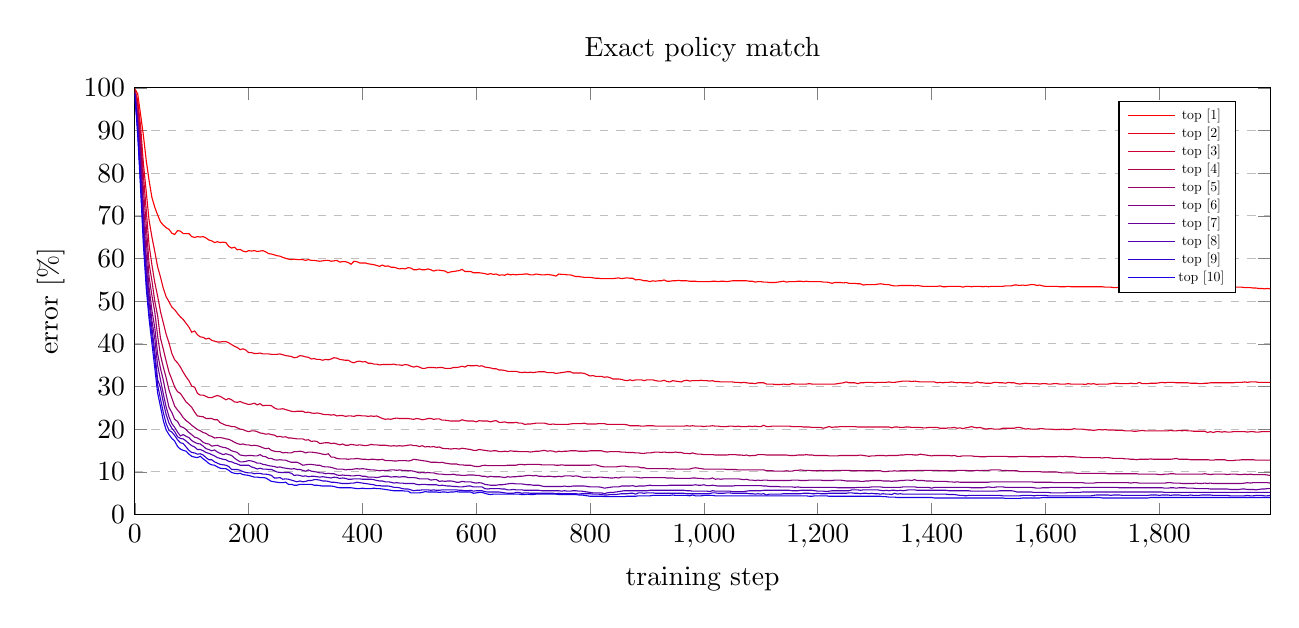
\begin{tikzpicture}
\begin{axis}[
   width=16cm,
   height=7cm,
   legend style={nodes={scale=0.5, transform shape}},
  title={Exact policy match},
  ylabel={error [\%]},
  ytick={0, 10, 20, 30, 40, 50, 60, 70, 80, 90, 100},
  xlabel={training step},
  xmin=0, xmax=1995,
  ymin=0, ymax=100,
  legend pos=north east,
  ymajorgrids=true,
  grid style=dashed,
]

\addplot[
  color=blue!0!red,
]
  coordinates {
  (0, 99.80079531669617)(5, 98.60557913780212)(10, 93.824702501297)(15, 88.84462118148804)(20, 82.96812772750854)(25, 78.2868504524231)(30, 74.30278658866882)(35, 72.01195359230042)(40, 70.21912336349487)(45, 68.62549781799316)(50, 67.82868504524231)(55, 67.23107695579529)(60, 66.83266758918762)(65, 65.93625545501709)(70, 65.63745141029358)(75, 66.53386354446411)(80, 66.43426418304443)(85, 65.83665609359741)(90, 65.83665609359741)(95, 65.83665609359741)(100, 65.13944268226624)(105, 64.9402379989624)(110, 65.13944268226624)(115, 65.03984332084656)(120, 65.13944268226624)(125, 64.84063863754272)(130, 64.34262990951538)(135, 64.14342522621155)(140, 63.74502182006836)(145, 63.944220542907715)(150, 63.74502182006836)(155, 63.84462118148804)(160, 63.74502182006836)(165, 62.84860372543335)(170, 62.45020031929016)(175, 62.649405002593994)(180, 62.051790952682495)(185, 62.15139627456665)(190, 61.752986907958984)(195, 61.55378222465515)(200, 61.85259222984314)(205, 61.752986907958984)(210, 61.85259222984314)(215, 61.65338754653931)(220, 61.752986907958984)(225, 61.85259222984314)(230, 61.55378222465515)(235, 61.15537881851196)(240, 61.055779457092285)(245, 60.85657477378845)(250, 60.65737009048462)(255, 60.55777072906494)(260, 60.25896668434143)(265, 60.0597620010376)(270, 59.860557317733765)(275, 59.76095795631409)(280, 59.860557317733765)(285, 59.76095795631409)(290, 59.76095795631409)(295, 59.76095795631409)(300, 59.561753273010254)(305, 59.76095795631409)(310, 59.561753273010254)(315, 59.561753273010254)(320, 59.462153911590576)(325, 59.36254858970642)(330, 59.462153911590576)(335, 59.561753273010254)(340, 59.561753273010254)(345, 59.36254858970642)(350, 59.462153911590576)(355, 59.561753273010254)(360, 59.16334390640259)(365, 59.26294922828674)(370, 59.26294922828674)(375, 59.06374454498291)(380, 58.66534113883972)(385, 59.36254858970642)(390, 59.26294922828674)(395, 58.96414518356323)(400, 58.96414518356323)(405, 58.96414518356323)(410, 58.7649405002594)(415, 58.66534113883972)(420, 58.565735816955566)(425, 58.36653113365173)(430, 58.16733241081238)(435, 58.46613645553589)(440, 58.16733241081238)(445, 58.266931772232056)(450, 57.968127727508545)(455, 57.968127727508545)(460, 57.76892304420471)(465, 57.56971836090088)(470, 57.669323682785034)(475, 57.56971836090088)(480, 57.86852836608887)(485, 57.76892304420471)(490, 57.37051963806152)(495, 57.37051963806152)(500, 57.56971836090088)(505, 57.37051963806152)(510, 57.37051963806152)(515, 57.56971836090088)(520, 57.37051963806152)(525, 57.07171559333801)(530, 57.27091431617737)(535, 57.27091431617737)(540, 57.17131495475769)(545, 57.07171559333801)(550, 56.67330622673035)(555, 56.87251091003418)(560, 56.97211027145386)(565, 57.07171559333801)(570, 57.17131495475769)(575, 57.4701189994812)(580, 56.97211027145386)(585, 56.97211027145386)(590, 56.97211027145386)(595, 56.67330622673035)(600, 56.67330622673035)(605, 56.67330622673035)(610, 56.57370686531067)(615, 56.474101543426514)(620, 56.27490282058716)(625, 56.474101543426514)(630, 56.27490282058716)(635, 56.374502182006836)(640, 56.075698137283325)(645, 56.175297498703)(650, 56.075698137283325)(655, 56.374502182006836)(660, 56.175297498703)(665, 56.27490282058716)(670, 56.175297498703)(675, 56.27490282058716)(680, 56.27490282058716)(685, 56.374502182006836)(690, 56.374502182006836)(695, 56.175297498703)(700, 56.175297498703)(705, 56.374502182006836)(710, 56.27490282058716)(715, 56.175297498703)(720, 56.175297498703)(725, 56.27490282058716)(730, 56.175297498703)(735, 56.075698137283325)(740, 55.87649345397949)(745, 56.374502182006836)(750, 56.27490282058716)(755, 56.27490282058716)(760, 56.175297498703)(765, 56.175297498703)(770, 55.97609281539917)(775, 55.776894092559814)(780, 55.776894092559814)(785, 55.67728877067566)(790, 55.57768940925598)(795, 55.57768940925598)(800, 55.57768940925598)(805, 55.478090047836304)(810, 55.37848472595215)(815, 55.37848472595215)(820, 55.27888536453247)(825, 55.27888536453247)(830, 55.27888536453247)(835, 55.27888536453247)(840, 55.27888536453247)(845, 55.37848472595215)(850, 55.478090047836304)(855, 55.27888536453247)(860, 55.37848472595215)(865, 55.478090047836304)(870, 55.37848472595215)(875, 55.37848472595215)(880, 54.98008131980896)(885, 55.07968068122864)(890, 54.98008131980896)(895, 54.78087663650513)(900, 54.78087663650513)(905, 54.581671953201294)(910, 54.78087663650513)(915, 54.68127727508545)(920, 54.78087663650513)(925, 54.78087663650513)(930, 54.98008131980896)(935, 54.68127727508545)(940, 54.68127727508545)(945, 54.78087663650513)(950, 54.78087663650513)(955, 54.880475997924805)(960, 54.78087663650513)(965, 54.78087663650513)(970, 54.78087663650513)(975, 54.68127727508545)(980, 54.68127727508545)(985, 54.68127727508545)(990, 54.581671953201294)(995, 54.581671953201294)(1000, 54.581671953201294)(1005, 54.581671953201294)(1010, 54.581671953201294)(1015, 54.68127727508545)(1020, 54.68127727508545)(1025, 54.581671953201294)(1030, 54.68127727508545)(1035, 54.68127727508545)(1040, 54.581671953201294)(1045, 54.68127727508545)(1050, 54.78087663650513)(1055, 54.78087663650513)(1060, 54.78087663650513)(1065, 54.78087663650513)(1070, 54.78087663650513)(1075, 54.78087663650513)(1080, 54.68127727508545)(1085, 54.68127727508545)(1090, 54.482072591781616)(1095, 54.581671953201294)(1100, 54.581671953201294)(1105, 54.482072591781616)(1110, 54.482072591781616)(1115, 54.38246726989746)(1120, 54.38246726989746)(1125, 54.38246726989746)(1130, 54.482072591781616)(1135, 54.581671953201294)(1140, 54.68127727508545)(1145, 54.482072591781616)(1150, 54.581671953201294)(1155, 54.581671953201294)(1160, 54.581671953201294)(1165, 54.68127727508545)(1170, 54.68127727508545)(1175, 54.581671953201294)(1180, 54.68127727508545)(1185, 54.581671953201294)(1190, 54.581671953201294)(1195, 54.581671953201294)(1200, 54.581671953201294)(1205, 54.581671953201294)(1210, 54.482072591781616)(1215, 54.482072591781616)(1220, 54.38246726989746)(1225, 54.183268547058105)(1230, 54.38246726989746)(1235, 54.38246726989746)(1240, 54.38246726989746)(1245, 54.28286790847778)(1250, 54.38246726989746)(1255, 54.183268547058105)(1260, 54.183268547058105)(1265, 54.183268547058105)(1270, 54.08366322517395)(1275, 54.08366322517395)(1280, 53.78485918045044)(1285, 53.884464502334595)(1290, 53.884464502334595)(1295, 53.884464502334595)(1300, 53.884464502334595)(1305, 53.98406386375427)(1310, 54.08366322517395)(1315, 53.98406386375427)(1320, 53.884464502334595)(1325, 53.884464502334595)(1330, 53.68525981903076)(1335, 53.585654497146606)(1340, 53.585654497146606)(1345, 53.68525981903076)(1350, 53.68525981903076)(1355, 53.68525981903076)(1360, 53.68525981903076)(1365, 53.68525981903076)(1370, 53.585654497146606)(1375, 53.68525981903076)(1380, 53.585654497146606)(1385, 53.48605513572693)(1390, 53.48605513572693)(1395, 53.48605513572693)(1400, 53.48605513572693)(1405, 53.48605513572693)(1410, 53.48605513572693)(1415, 53.585654497146606)(1420, 53.38645577430725)(1425, 53.38645577430725)(1430, 53.48605513572693)(1435, 53.48605513572693)(1440, 53.48605513572693)(1445, 53.48605513572693)(1450, 53.48605513572693)(1455, 53.286850452423096)(1460, 53.48605513572693)(1465, 53.48605513572693)(1470, 53.38645577430725)(1475, 53.48605513572693)(1480, 53.48605513572693)(1485, 53.48605513572693)(1490, 53.38645577430725)(1495, 53.48605513572693)(1500, 53.38645577430725)(1505, 53.48605513572693)(1510, 53.48605513572693)(1515, 53.48605513572693)(1520, 53.48605513572693)(1525, 53.48605513572693)(1530, 53.585654497146606)(1535, 53.585654497146606)(1540, 53.585654497146606)(1545, 53.78485918045044)(1550, 53.78485918045044)(1555, 53.68525981903076)(1560, 53.78485918045044)(1565, 53.68525981903076)(1570, 53.78485918045044)(1575, 53.884464502334595)(1580, 53.884464502334595)(1585, 53.68525981903076)(1590, 53.78485918045044)(1595, 53.585654497146606)(1600, 53.48605513572693)(1605, 53.48605513572693)(1610, 53.48605513572693)(1615, 53.48605513572693)(1620, 53.48605513572693)(1625, 53.38645577430725)(1630, 53.38645577430725)(1635, 53.38645577430725)(1640, 53.48605513572693)(1645, 53.38645577430725)(1650, 53.38645577430725)(1655, 53.38645577430725)(1660, 53.38645577430725)(1665, 53.38645577430725)(1670, 53.38645577430725)(1675, 53.38645577430725)(1680, 53.38645577430725)(1685, 53.38645577430725)(1690, 53.38645577430725)(1695, 53.38645577430725)(1700, 53.38645577430725)(1705, 53.286850452423096)(1710, 53.286850452423096)(1715, 53.286850452423096)(1720, 53.18725109100342)(1725, 53.18725109100342)(1730, 53.286850452423096)(1735, 53.18725109100342)(1740, 53.18725109100342)(1745, 53.18725109100342)(1750, 53.08765172958374)(1755, 52.988046407699585)(1760, 53.08765172958374)(1765, 53.08765172958374)(1770, 53.08765172958374)(1775, 52.988046407699585)(1780, 53.18725109100342)(1785, 53.18725109100342)(1790, 53.18725109100342)(1795, 53.18725109100342)(1800, 53.18725109100342)(1805, 53.18725109100342)(1810, 53.18725109100342)(1815, 53.18725109100342)(1820, 53.286850452423096)(1825, 53.286850452423096)(1830, 53.286850452423096)(1835, 53.286850452423096)(1840, 53.286850452423096)(1845, 53.286850452423096)(1850, 53.286850452423096)(1855, 53.286850452423096)(1860, 53.286850452423096)(1865, 53.286850452423096)(1870, 53.286850452423096)(1875, 53.38645577430725)(1880, 53.38645577430725)(1885, 53.38645577430725)(1890, 53.38645577430725)(1895, 53.38645577430725)(1900, 53.38645577430725)(1905, 53.38645577430725)(1910, 53.38645577430725)(1915, 53.286850452423096)(1920, 53.286850452423096)(1925, 53.286850452423096)(1930, 53.286850452423096)(1935, 53.286850452423096)(1940, 53.286850452423096)(1945, 53.286850452423096)(1950, 53.18725109100342)(1955, 53.18725109100342)(1960, 53.18725109100342)(1965, 53.08765172958374)(1970, 53.08765172958374)(1975, 52.988046407699585)(1980, 52.988046407699585)(1985, 52.88844704627991)(1990, 52.988046407699585)(1995, 52.88844704627991)
  };
\addlegendentry{top [1]};
\addplot[
  color=blue!10!red,
]
  coordinates {
  (0, 99.70119595527649)(5, 97.01195359230042)(10, 91.13546013832092)(15, 82.27091431617737)(20, 75.59760808944702)(25, 68.92430186271667)(30, 65.03984332084656)(35, 61.65338754653931)(40, 58.06772708892822)(45, 55.67728877067566)(50, 52.988046407699585)(55, 50.99601745605469)(60, 49.90039765834808)(65, 48.605579137802124)(70, 48.007968068122864)(75, 47.11155295372009)(80, 46.31474018096924)(85, 45.71713209152222)(90, 44.820716977119446)(95, 43.924301862716675)(100, 42.72908270359039)(105, 43.02788972854614)(110, 42.13147461414337)(115, 41.63346588611603)(120, 41.53386354446411)(125, 41.135457158088684)(130, 41.33466184139252)(135, 40.83665311336517)(140, 40.63745141029358)(145, 40.438246726989746)(150, 40.438246726989746)(155, 40.53784906864166)(160, 40.53784906864166)(165, 40.23904502391815)(170, 39.840638637542725)(175, 39.4422322511673)(180, 39.14342522621155)(185, 38.64541947841644)(190, 38.84462118148804)(195, 38.545817136764526)(200, 37.948206067085266)(205, 37.948206067085266)(210, 37.74900436401367)(215, 37.74900436401367)(220, 37.84860670566559)(225, 37.649402022361755)(230, 37.649402022361755)(235, 37.649402022361755)(240, 37.54979968070984)(245, 37.54979968070984)(250, 37.54979968070984)(255, 37.649402022361755)(260, 37.45020031929016)(265, 37.25099563598633)(270, 37.15139329433441)(275, 37.051793932914734)(280, 36.752986907958984)(285, 36.8525892496109)(290, 37.25099563598633)(295, 37.15139329433441)(300, 36.95219159126282)(305, 36.8525892496109)(310, 36.454182863235474)(315, 36.55378520488739)(320, 36.35458052158356)(325, 36.35458052158356)(330, 36.15537881851196)(335, 36.35458052158356)(340, 36.25498116016388)(345, 36.454182863235474)(350, 36.752986907958984)(355, 36.65338754653931)(360, 36.35458052158356)(365, 36.25498116016388)(370, 36.15537881851196)(375, 36.15537881851196)(380, 35.756972432136536)(385, 35.5577677488327)(390, 35.85657477378845)(395, 35.95617413520813)(400, 35.756972432136536)(405, 35.85657477378845)(410, 35.458168387413025)(415, 35.458168387413025)(420, 35.25896370410919)(425, 35.25896370410919)(430, 35.0597620010376)(435, 35.159361362457275)(440, 35.159361362457275)(445, 35.159361362457275)(450, 35.159361362457275)(455, 35.25896370410919)(460, 35.0597620010376)(465, 35.0597620010376)(470, 34.96015965938568)(475, 35.159361362457275)(480, 35.0597620010376)(485, 34.76095497608185)(490, 34.561753273010254)(495, 34.76095497608185)(500, 34.561753273010254)(505, 34.26294922828674)(510, 34.26294922828674)(515, 34.46215093135834)(520, 34.46215093135834)(525, 34.46215093135834)(530, 34.36254858970642)(535, 34.46215093135834)(540, 34.46215093135834)(545, 34.26294922828674)(550, 34.26294922828674)(555, 34.26294922828674)(560, 34.46215093135834)(565, 34.46215093135834)(570, 34.561753273010254)(575, 34.76095497608185)(580, 34.561753273010254)(585, 34.96015965938568)(590, 34.860557317733765)(595, 34.860557317733765)(600, 34.96015965938568)(605, 34.76095497608185)(610, 34.860557317733765)(615, 34.561753273010254)(620, 34.46215093135834)(625, 34.36254858970642)(630, 34.16334688663483)(635, 34.16334688663483)(640, 33.864542841911316)(645, 33.864542841911316)(650, 33.7649405002594)(655, 33.565735816955566)(660, 33.565735816955566)(665, 33.565735816955566)(670, 33.565735816955566)(675, 33.36653411388397)(680, 33.266931772232056)(685, 33.36653411388397)(690, 33.266931772232056)(695, 33.36653411388397)(700, 33.266931772232056)(705, 33.36653411388397)(710, 33.46613645553589)(715, 33.46613645553589)(720, 33.46613645553589)(725, 33.266931772232056)(730, 33.266931772232056)(735, 33.266931772232056)(740, 33.06773006916046)(745, 33.16732943058014)(750, 33.266931772232056)(755, 33.36653411388397)(760, 33.46613645553589)(765, 33.46613645553589)(770, 33.16732943058014)(775, 33.16732943058014)(780, 33.16732943058014)(785, 33.16732943058014)(790, 33.06773006916046)(795, 32.76892304420471)(800, 32.4701189994812)(805, 32.56972134113312)(810, 32.370516657829285)(815, 32.370516657829285)(820, 32.370516657829285)(825, 32.17131495475769)(830, 32.27091729640961)(835, 32.071712613105774)(840, 31.772908568382263)(845, 31.772908568382263)(850, 31.772908568382263)(855, 31.673306226730347)(860, 31.474104523658752)(865, 31.374502182006836)(870, 31.57370388507843)(875, 31.374502182006836)(880, 31.57370388507843)(885, 31.57370388507843)(890, 31.57370388507843)(895, 31.374502182006836)(900, 31.57370388507843)(905, 31.57370388507843)(910, 31.57370388507843)(915, 31.374502182006836)(920, 31.27489984035492)(925, 31.27489984035492)(930, 31.474104523658752)(935, 31.175297498703003)(940, 31.075698137283325)(945, 31.374502182006836)(950, 31.27489984035492)(955, 31.175297498703003)(960, 31.075698137283325)(965, 31.374502182006836)(970, 31.474104523658752)(975, 31.27489984035492)(980, 31.374502182006836)(985, 31.374502182006836)(990, 31.374502182006836)(995, 31.474104523658752)(1000, 31.374502182006836)(1005, 31.374502182006836)(1010, 31.27489984035492)(1015, 31.374502182006836)(1020, 31.175297498703003)(1025, 31.175297498703003)(1030, 31.075698137283325)(1035, 31.075698137283325)(1040, 31.075698137283325)(1045, 31.075698137283325)(1050, 31.075698137283325)(1055, 30.97609579563141)(1060, 30.97609579563141)(1065, 30.876493453979492)(1070, 30.97609579563141)(1075, 30.876493453979492)(1080, 30.776891112327576)(1085, 30.776891112327576)(1090, 30.677291750907898)(1095, 30.876493453979492)(1100, 30.876493453979492)(1105, 30.876493453979492)(1110, 30.57768940925598)(1115, 30.57768940925598)(1120, 30.57768940925598)(1125, 30.478087067604065)(1130, 30.478087067604065)(1135, 30.478087067604065)(1140, 30.57768940925598)(1145, 30.478087067604065)(1150, 30.478087067604065)(1155, 30.677291750907898)(1160, 30.57768940925598)(1165, 30.57768940925598)(1170, 30.57768940925598)(1175, 30.57768940925598)(1180, 30.57768940925598)(1185, 30.677291750907898)(1190, 30.57768940925598)(1195, 30.57768940925598)(1200, 30.57768940925598)(1205, 30.57768940925598)(1210, 30.57768940925598)(1215, 30.57768940925598)(1220, 30.57768940925598)(1225, 30.57768940925598)(1230, 30.57768940925598)(1235, 30.677291750907898)(1240, 30.776891112327576)(1245, 30.876493453979492)(1250, 31.075698137283325)(1255, 30.876493453979492)(1260, 30.876493453979492)(1265, 30.876493453979492)(1270, 30.677291750907898)(1275, 30.876493453979492)(1280, 30.876493453979492)(1285, 30.97609579563141)(1290, 30.97609579563141)(1295, 30.97609579563141)(1300, 30.876493453979492)(1305, 30.97609579563141)(1310, 30.97609579563141)(1315, 30.97609579563141)(1320, 30.97609579563141)(1325, 31.075698137283325)(1330, 30.97609579563141)(1335, 30.97609579563141)(1340, 31.075698137283325)(1345, 31.175297498703003)(1350, 31.27489984035492)(1355, 31.27489984035492)(1360, 31.27489984035492)(1365, 31.175297498703003)(1370, 31.27489984035492)(1375, 31.175297498703003)(1380, 31.075698137283325)(1385, 31.075698137283325)(1390, 31.075698137283325)(1395, 31.075698137283325)(1400, 31.075698137283325)(1405, 31.075698137283325)(1410, 30.876493453979492)(1415, 30.97609579563141)(1420, 30.876493453979492)(1425, 30.97609579563141)(1430, 30.97609579563141)(1435, 31.075698137283325)(1440, 30.97609579563141)(1445, 30.876493453979492)(1450, 30.97609579563141)(1455, 30.876493453979492)(1460, 30.876493453979492)(1465, 30.876493453979492)(1470, 30.776891112327576)(1475, 30.876493453979492)(1480, 31.075698137283325)(1485, 30.876493453979492)(1490, 30.876493453979492)(1495, 30.776891112327576)(1500, 30.776891112327576)(1505, 30.776891112327576)(1510, 30.97609579563141)(1515, 30.97609579563141)(1520, 30.876493453979492)(1525, 30.876493453979492)(1530, 30.776891112327576)(1535, 30.97609579563141)(1540, 30.876493453979492)(1545, 30.876493453979492)(1550, 30.677291750907898)(1555, 30.57768940925598)(1560, 30.677291750907898)(1565, 30.776891112327576)(1570, 30.677291750907898)(1575, 30.677291750907898)(1580, 30.677291750907898)(1585, 30.677291750907898)(1590, 30.57768940925598)(1595, 30.677291750907898)(1600, 30.677291750907898)(1605, 30.57768940925598)(1610, 30.57768940925598)(1615, 30.677291750907898)(1620, 30.677291750907898)(1625, 30.57768940925598)(1630, 30.57768940925598)(1635, 30.57768940925598)(1640, 30.677291750907898)(1645, 30.57768940925598)(1650, 30.57768940925598)(1655, 30.57768940925598)(1660, 30.57768940925598)(1665, 30.57768940925598)(1670, 30.478087067604065)(1675, 30.677291750907898)(1680, 30.57768940925598)(1685, 30.677291750907898)(1690, 30.478087067604065)(1695, 30.57768940925598)(1700, 30.57768940925598)(1705, 30.57768940925598)(1710, 30.57768940925598)(1715, 30.677291750907898)(1720, 30.776891112327576)(1725, 30.776891112327576)(1730, 30.677291750907898)(1735, 30.677291750907898)(1740, 30.677291750907898)(1745, 30.677291750907898)(1750, 30.776891112327576)(1755, 30.677291750907898)(1760, 30.677291750907898)(1765, 30.97609579563141)(1770, 30.677291750907898)(1775, 30.677291750907898)(1780, 30.677291750907898)(1785, 30.776891112327576)(1790, 30.776891112327576)(1795, 30.776891112327576)(1800, 30.876493453979492)(1805, 30.97609579563141)(1810, 30.876493453979492)(1815, 30.97609579563141)(1820, 30.97609579563141)(1825, 30.97609579563141)(1830, 30.876493453979492)(1835, 30.876493453979492)(1840, 30.876493453979492)(1845, 30.876493453979492)(1850, 30.876493453979492)(1855, 30.776891112327576)(1860, 30.776891112327576)(1865, 30.776891112327576)(1870, 30.677291750907898)(1875, 30.677291750907898)(1880, 30.776891112327576)(1885, 30.776891112327576)(1890, 30.876493453979492)(1895, 30.876493453979492)(1900, 30.876493453979492)(1905, 30.876493453979492)(1910, 30.876493453979492)(1915, 30.876493453979492)(1920, 30.876493453979492)(1925, 30.876493453979492)(1930, 30.876493453979492)(1935, 30.97609579563141)(1940, 30.97609579563141)(1945, 30.97609579563141)(1950, 31.075698137283325)(1955, 30.97609579563141)(1960, 31.075698137283325)(1965, 31.075698137283325)(1970, 31.075698137283325)(1975, 30.97609579563141)(1980, 30.97609579563141)(1985, 30.97609579563141)(1990, 30.97609579563141)(1995, 30.97609579563141)
  };
\addlegendentry{top [2]};
\addplot[
  color=blue!20!red,
]
  coordinates {
  (0, 99.50199127197266)(5, 96.01593613624573)(10, 88.94422054290771)(15, 79.48207259178162)(20, 71.31474018096924)(25, 63.14740777015686)(30, 58.46613645553589)(35, 54.38246726989746)(40, 51.19521617889404)(45, 47.60956168174744)(50, 44.92031931877136)(55, 42.23107695579529)(60, 40.23904502391815)(65, 37.74900436401367)(70, 36.25498116016388)(75, 35.5577677488327)(80, 34.561753273010254)(85, 33.36653411388397)(90, 32.27091729640961)(95, 31.374502182006836)(100, 30.079680681228638)(105, 29.880478978157043)(110, 28.386452794075012)(115, 27.988046407699585)(120, 27.988046407699585)(125, 27.689242362976074)(130, 27.390438318252563)(135, 27.390438318252563)(140, 27.689242362976074)(145, 27.888447046279907)(150, 27.689242362976074)(155, 27.290835976600647)(160, 26.89242959022522)(165, 27.19123363494873)(170, 26.89242959022522)(175, 26.394420862197876)(180, 26.2948215007782)(185, 26.494023203849792)(190, 26.19521915912628)(195, 25.99601447582245)(200, 25.796812772750854)(205, 25.89641511440277)(210, 26.095616817474365)(215, 25.697210431098938)(220, 25.99601447582245)(225, 25.498008728027344)(230, 25.59760808944702)(235, 25.59760808944702)(240, 25.498008728027344)(245, 25.0)(250, 24.70119595527649)(255, 24.70119595527649)(260, 24.800796806812286)(265, 24.601593613624573)(270, 24.40239042043686)(275, 24.203187227249146)(280, 24.10358637571335)(285, 24.203187227249146)(290, 24.203187227249146)(295, 24.203187227249146)(300, 23.904383182525635)(305, 24.003984034061432)(310, 23.80478084087372)(315, 23.70517998933792)(320, 23.80478084087372)(325, 23.70517998933792)(330, 23.505976796150208)(335, 23.40637445449829)(340, 23.40637445449829)(345, 23.306773602962494)(350, 23.40637445449829)(355, 23.10757040977478)(360, 23.207171261310577)(365, 23.207171261310577)(370, 23.007968068122864)(375, 23.10757040977478)(380, 23.10757040977478)(385, 23.007968068122864)(390, 23.207171261310577)(395, 23.207171261310577)(400, 23.10757040977478)(405, 23.10757040977478)(410, 23.007968068122864)(415, 23.10757040977478)(420, 23.007968068122864)(425, 23.10757040977478)(430, 22.80876487493515)(435, 22.50996083021164)(440, 22.310757637023926)(445, 22.410358488559723)(450, 22.310757637023926)(455, 22.50996083021164)(460, 22.609561681747437)(465, 22.50996083021164)(470, 22.50996083021164)(475, 22.50996083021164)(480, 22.50996083021164)(485, 22.410358488559723)(490, 22.310757637023926)(495, 22.50996083021164)(500, 22.410358488559723)(505, 22.21115529537201)(510, 22.310757637023926)(515, 22.50996083021164)(520, 22.50996083021164)(525, 22.310757637023926)(530, 22.410358488559723)(535, 22.410358488559723)(540, 22.111554443836212)(545, 22.111554443836212)(550, 22.011952102184296)(555, 21.9123512506485)(560, 21.9123512506485)(565, 21.9123512506485)(570, 21.9123512506485)(575, 22.21115529537201)(580, 22.011952102184296)(585, 21.9123512506485)(590, 21.9123512506485)(595, 21.9123512506485)(600, 21.713148057460785)(605, 22.011952102184296)(610, 21.9123512506485)(615, 21.9123512506485)(620, 21.9123512506485)(625, 21.713148057460785)(630, 21.9123512506485)(635, 22.011952102184296)(640, 21.61354571580887)(645, 21.61354571580887)(650, 21.713148057460785)(655, 21.51394486427307)(660, 21.51394486427307)(665, 21.51394486427307)(670, 21.61354571580887)(675, 21.414342522621155)(680, 21.414342522621155)(685, 21.115538477897644)(690, 21.21513932943344)(695, 21.21513932943344)(700, 21.314741671085358)(705, 21.414342522621155)(710, 21.414342522621155)(715, 21.414342522621155)(720, 21.414342522621155)(725, 21.21513932943344)(730, 21.115538477897644)(735, 21.21513932943344)(740, 21.115538477897644)(745, 21.115538477897644)(750, 21.115538477897644)(755, 21.115538477897644)(760, 21.115538477897644)(765, 21.21513932943344)(770, 21.314741671085358)(775, 21.314741671085358)(780, 21.314741671085358)(785, 21.314741671085358)(790, 21.414342522621155)(795, 21.21513932943344)(800, 21.21513932943344)(805, 21.21513932943344)(810, 21.21513932943344)(815, 21.314741671085358)(820, 21.314741671085358)(825, 21.314741671085358)(830, 21.115538477897644)(835, 21.115538477897644)(840, 21.115538477897644)(845, 21.115538477897644)(850, 21.115538477897644)(855, 21.115538477897644)(860, 21.115538477897644)(865, 21.015936136245728)(870, 20.816732943058014)(875, 20.816732943058014)(880, 20.816732943058014)(885, 20.816732943058014)(890, 20.717132091522217)(895, 20.717132091522217)(900, 20.816732943058014)(905, 20.816732943058014)(910, 20.816732943058014)(915, 20.717132091522217)(920, 20.717132091522217)(925, 20.717132091522217)(930, 20.717132091522217)(935, 20.717132091522217)(940, 20.717132091522217)(945, 20.717132091522217)(950, 20.717132091522217)(955, 20.717132091522217)(960, 20.717132091522217)(965, 20.717132091522217)(970, 20.816732943058014)(975, 20.717132091522217)(980, 20.816732943058014)(985, 20.717132091522217)(990, 20.717132091522217)(995, 20.717132091522217)(1000, 20.6175297498703)(1005, 20.717132091522217)(1010, 20.717132091522217)(1015, 20.816732943058014)(1020, 20.717132091522217)(1025, 20.717132091522217)(1030, 20.6175297498703)(1035, 20.6175297498703)(1040, 20.6175297498703)(1045, 20.717132091522217)(1050, 20.717132091522217)(1055, 20.6175297498703)(1060, 20.717132091522217)(1065, 20.6175297498703)(1070, 20.6175297498703)(1075, 20.6175297498703)(1080, 20.717132091522217)(1085, 20.6175297498703)(1090, 20.717132091522217)(1095, 20.6175297498703)(1100, 20.6175297498703)(1105, 20.91633528470993)(1110, 20.6175297498703)(1115, 20.6175297498703)(1120, 20.717132091522217)(1125, 20.717132091522217)(1130, 20.717132091522217)(1135, 20.717132091522217)(1140, 20.717132091522217)(1145, 20.717132091522217)(1150, 20.717132091522217)(1155, 20.6175297498703)(1160, 20.6175297498703)(1165, 20.6175297498703)(1170, 20.6175297498703)(1175, 20.517928898334503)(1180, 20.517928898334503)(1185, 20.517928898334503)(1190, 20.418326556682587)(1195, 20.418326556682587)(1200, 20.418326556682587)(1205, 20.418326556682587)(1210, 20.219123363494873)(1215, 20.418326556682587)(1220, 20.6175297498703)(1225, 20.418326556682587)(1230, 20.517928898334503)(1235, 20.517928898334503)(1240, 20.6175297498703)(1245, 20.6175297498703)(1250, 20.6175297498703)(1255, 20.6175297498703)(1260, 20.6175297498703)(1265, 20.6175297498703)(1270, 20.517928898334503)(1275, 20.517928898334503)(1280, 20.517928898334503)(1285, 20.517928898334503)(1290, 20.517928898334503)(1295, 20.517928898334503)(1300, 20.517928898334503)(1305, 20.517928898334503)(1310, 20.517928898334503)(1315, 20.517928898334503)(1320, 20.517928898334503)(1325, 20.517928898334503)(1330, 20.31872570514679)(1335, 20.517928898334503)(1340, 20.517928898334503)(1345, 20.418326556682587)(1350, 20.418326556682587)(1355, 20.517928898334503)(1360, 20.517928898334503)(1365, 20.418326556682587)(1370, 20.418326556682587)(1375, 20.418326556682587)(1380, 20.418326556682587)(1385, 20.31872570514679)(1390, 20.31872570514679)(1395, 20.418326556682587)(1400, 20.418326556682587)(1405, 20.418326556682587)(1410, 20.418326556682587)(1415, 20.219123363494873)(1420, 20.219123363494873)(1425, 20.219123363494873)(1430, 20.31872570514679)(1435, 20.31872570514679)(1440, 20.418326556682587)(1445, 20.219123363494873)(1450, 20.31872570514679)(1455, 20.119522511959076)(1460, 20.31872570514679)(1465, 20.418326556682587)(1470, 20.6175297498703)(1475, 20.418326556682587)(1480, 20.31872570514679)(1485, 20.418326556682587)(1490, 20.219123363494873)(1495, 20.01992017030716)(1500, 20.119522511959076)(1505, 20.119522511959076)(1510, 20.01992017030716)(1515, 20.01992017030716)(1520, 20.01992017030716)(1525, 20.219123363494873)(1530, 20.219123363494873)(1535, 20.219123363494873)(1540, 20.219123363494873)(1545, 20.219123363494873)(1550, 20.418326556682587)(1555, 20.418326556682587)(1560, 20.219123363494873)(1565, 20.01992017030716)(1570, 20.119522511959076)(1575, 20.01992017030716)(1580, 20.01992017030716)(1585, 20.01992017030716)(1590, 20.119522511959076)(1595, 20.119522511959076)(1600, 20.01992017030716)(1605, 20.01992017030716)(1610, 20.01992017030716)(1615, 19.920319318771362)(1620, 19.920319318771362)(1625, 19.920319318771362)(1630, 20.01992017030716)(1635, 19.920319318771362)(1640, 19.920319318771362)(1645, 19.920319318771362)(1650, 20.119522511959076)(1655, 20.01992017030716)(1660, 20.01992017030716)(1665, 20.01992017030716)(1670, 19.920319318771362)(1675, 19.820716977119446)(1680, 19.820716977119446)(1685, 19.72111612558365)(1690, 19.820716977119446)(1695, 19.920319318771362)(1700, 19.820716977119446)(1705, 19.920319318771362)(1710, 19.820716977119446)(1715, 19.820716977119446)(1720, 19.820716977119446)(1725, 19.72111612558365)(1730, 19.72111612558365)(1735, 19.72111612558365)(1740, 19.621513783931732)(1745, 19.621513783931732)(1750, 19.621513783931732)(1755, 19.521912932395935)(1760, 19.521912932395935)(1765, 19.621513783931732)(1770, 19.72111612558365)(1775, 19.621513783931732)(1780, 19.621513783931732)(1785, 19.621513783931732)(1790, 19.621513783931732)(1795, 19.621513783931732)(1800, 19.621513783931732)(1805, 19.621513783931732)(1810, 19.621513783931732)(1815, 19.621513783931732)(1820, 19.72111612558365)(1825, 19.621513783931732)(1830, 19.621513783931732)(1835, 19.72111612558365)(1840, 19.621513783931732)(1845, 19.72111612558365)(1850, 19.621513783931732)(1855, 19.621513783931732)(1860, 19.521912932395935)(1865, 19.521912932395935)(1870, 19.521912932395935)(1875, 19.521912932395935)(1880, 19.521912932395935)(1885, 19.223107397556305)(1890, 19.42231059074402)(1895, 19.223107397556305)(1900, 19.42231059074402)(1905, 19.42231059074402)(1910, 19.32270973920822)(1915, 19.42231059074402)(1920, 19.32270973920822)(1925, 19.32270973920822)(1930, 19.42231059074402)(1935, 19.42231059074402)(1940, 19.42231059074402)(1945, 19.42231059074402)(1950, 19.42231059074402)(1955, 19.32270973920822)(1960, 19.42231059074402)(1965, 19.42231059074402)(1970, 19.32270973920822)(1975, 19.32270973920822)(1980, 19.42231059074402)(1985, 19.42231059074402)(1990, 19.42231059074402)(1995, 19.42231059074402)
  };
\addlegendentry{top [3]};
\addplot[
  color=blue!30!red,
]
  coordinates {
  (0, 99.30278658866882)(5, 94.22310590744019)(10, 87.45020031929016)(15, 76.19521617889404)(20, 67.82868504524231)(25, 58.7649405002594)(30, 54.78087663650513)(35, 50.0)(40, 46.61354720592499)(45, 41.33466184139252)(50, 38.74501883983612)(55, 35.95617413520813)(60, 33.36653411388397)(65, 31.673306226730347)(70, 29.880478978157043)(75, 28.78485918045044)(80, 28.386452794075012)(85, 27.390438318252563)(90, 26.394420862197876)(95, 25.796812772750854)(100, 25.099602341651917)(105, 24.003984034061432)(110, 23.10757040977478)(115, 23.007968068122864)(120, 22.908367216587067)(125, 22.50996083021164)(130, 22.50996083021164)(135, 22.50996083021164)(140, 22.21115529537201)(145, 22.21115529537201)(150, 21.51394486427307)(155, 21.21513932943344)(160, 20.91633528470993)(165, 20.816732943058014)(170, 20.6175297498703)(175, 20.6175297498703)(180, 20.31872570514679)(185, 20.01992017030716)(190, 19.920319318771362)(195, 19.621513783931732)(200, 19.42231059074402)(205, 19.621513783931732)(210, 19.621513783931732)(215, 19.42231059074402)(220, 19.123506546020508)(225, 19.02390420436859)(230, 18.824701011180878)(235, 18.924303352832794)(240, 18.72510015964508)(245, 18.625497817993164)(250, 18.227091431617737)(255, 18.326693773269653)(260, 18.12749058008194)(265, 18.227091431617737)(270, 17.928287386894226)(275, 17.928287386894226)(280, 17.82868504524231)(285, 17.729084193706512)(290, 17.729084193706512)(295, 17.729084193706512)(300, 17.430278658866882)(305, 17.5298810005188)(310, 17.13147461414337)(315, 17.23107546567917)(320, 17.13147461414337)(325, 16.633465886116028)(330, 16.733068227767944)(335, 16.83266907930374)(340, 16.83266907930374)(345, 16.633465886116028)(350, 16.733068227767944)(355, 16.53386503458023)(360, 16.334661841392517)(365, 16.53386503458023)(370, 16.2350594997406)(375, 16.2350594997406)(380, 16.434262692928314)(385, 16.334661841392517)(390, 16.2350594997406)(395, 16.334661841392517)(400, 16.2350594997406)(405, 16.135458648204803)(410, 16.2350594997406)(415, 16.434262692928314)(420, 16.334661841392517)(425, 16.334661841392517)(430, 16.2350594997406)(435, 16.2350594997406)(440, 16.2350594997406)(445, 16.135458648204803)(450, 16.035856306552887)(455, 16.135458648204803)(460, 16.035856306552887)(465, 16.135458648204803)(470, 16.035856306552887)(475, 16.135458648204803)(480, 16.2350594997406)(485, 16.334661841392517)(490, 16.135458648204803)(495, 16.135458648204803)(500, 15.93625545501709)(505, 16.135458648204803)(510, 15.836653113365173)(515, 15.93625545501709)(520, 15.836653113365173)(525, 15.93625545501709)(530, 15.737052261829376)(535, 15.836653113365173)(540, 15.537849068641663)(545, 15.438246726989746)(550, 15.438246726989746)(555, 15.338645875453949)(560, 15.438246726989746)(565, 15.438246726989746)(570, 15.338645875453949)(575, 15.537849068641663)(580, 15.438246726989746)(585, 15.338645875453949)(590, 15.239043533802032)(595, 15.039840340614319)(600, 15.039840340614319)(605, 15.239043533802032)(610, 15.139442682266235)(615, 15.039840340614319)(620, 14.940239489078522)(625, 14.840637147426605)(630, 14.940239489078522)(635, 14.940239489078522)(640, 14.741036295890808)(645, 14.741036295890808)(650, 14.840637147426605)(655, 14.741036295890808)(660, 14.940239489078522)(665, 14.840637147426605)(670, 14.840637147426605)(675, 14.741036295890808)(680, 14.741036295890808)(685, 14.741036295890808)(690, 14.741036295890808)(695, 14.641433954238892)(700, 14.741036295890808)(705, 14.840637147426605)(710, 14.840637147426605)(715, 14.940239489078522)(720, 15.039840340614319)(725, 14.840637147426605)(730, 14.940239489078522)(735, 14.840637147426605)(740, 14.641433954238892)(745, 14.840637147426605)(750, 14.741036295890808)(755, 14.840637147426605)(760, 14.840637147426605)(765, 14.940239489078522)(770, 14.940239489078522)(775, 14.940239489078522)(780, 14.840637147426605)(785, 14.840637147426605)(790, 14.840637147426605)(795, 14.840637147426605)(800, 14.940239489078522)(805, 14.940239489078522)(810, 14.940239489078522)(815, 14.940239489078522)(820, 14.940239489078522)(825, 14.741036295890808)(830, 14.641433954238892)(835, 14.741036295890808)(840, 14.741036295890808)(845, 14.741036295890808)(850, 14.741036295890808)(855, 14.641433954238892)(860, 14.641433954238892)(865, 14.541833102703094)(870, 14.541833102703094)(875, 14.541833102703094)(880, 14.442230761051178)(885, 14.442230761051178)(890, 14.34262990951538)(895, 14.34262990951538)(900, 14.442230761051178)(905, 14.442230761051178)(910, 14.541833102703094)(915, 14.641433954238892)(920, 14.641433954238892)(925, 14.541833102703094)(930, 14.641433954238892)(935, 14.541833102703094)(940, 14.541833102703094)(945, 14.541833102703094)(950, 14.641433954238892)(955, 14.541833102703094)(960, 14.541833102703094)(965, 14.34262990951538)(970, 14.34262990951538)(975, 14.243027567863464)(980, 14.442230761051178)(985, 14.243027567863464)(990, 14.143426716327667)(995, 14.143426716327667)(1000, 14.04382437467575)(1005, 14.04382437467575)(1010, 14.04382437467575)(1015, 14.04382437467575)(1020, 13.944223523139954)(1025, 13.944223523139954)(1030, 13.944223523139954)(1035, 13.944223523139954)(1040, 13.944223523139954)(1045, 14.04382437467575)(1050, 14.04382437467575)(1055, 14.04382437467575)(1060, 13.944223523139954)(1065, 13.944223523139954)(1070, 13.844621181488037)(1075, 13.944223523139954)(1080, 13.74502032995224)(1085, 13.844621181488037)(1090, 13.844621181488037)(1095, 14.04382437467575)(1100, 14.04382437467575)(1105, 14.04382437467575)(1110, 13.944223523139954)(1115, 13.944223523139954)(1120, 13.944223523139954)(1125, 13.944223523139954)(1130, 13.944223523139954)(1135, 13.944223523139954)(1140, 13.944223523139954)(1145, 13.944223523139954)(1150, 13.844621181488037)(1155, 13.844621181488037)(1160, 13.844621181488037)(1165, 13.944223523139954)(1170, 13.944223523139954)(1175, 13.944223523139954)(1180, 14.04382437467575)(1185, 13.944223523139954)(1190, 13.944223523139954)(1195, 13.844621181488037)(1200, 13.844621181488037)(1205, 13.844621181488037)(1210, 13.844621181488037)(1215, 13.844621181488037)(1220, 13.74502032995224)(1225, 13.74502032995224)(1230, 13.74502032995224)(1235, 13.74502032995224)(1240, 13.844621181488037)(1245, 13.844621181488037)(1250, 13.844621181488037)(1255, 13.844621181488037)(1260, 13.844621181488037)(1265, 13.844621181488037)(1270, 13.844621181488037)(1275, 13.944223523139954)(1280, 13.844621181488037)(1285, 13.74502032995224)(1290, 13.645417988300323)(1295, 13.74502032995224)(1300, 13.74502032995224)(1305, 13.844621181488037)(1310, 13.844621181488037)(1315, 13.844621181488037)(1320, 13.74502032995224)(1325, 13.844621181488037)(1330, 13.844621181488037)(1335, 13.844621181488037)(1340, 13.844621181488037)(1345, 13.944223523139954)(1350, 13.944223523139954)(1355, 14.04382437467575)(1360, 14.04382437467575)(1365, 14.04382437467575)(1370, 13.944223523139954)(1375, 13.944223523139954)(1380, 14.143426716327667)(1385, 14.04382437467575)(1390, 13.944223523139954)(1395, 13.844621181488037)(1400, 13.74502032995224)(1405, 13.844621181488037)(1410, 13.844621181488037)(1415, 13.844621181488037)(1420, 13.844621181488037)(1425, 13.844621181488037)(1430, 13.844621181488037)(1435, 13.74502032995224)(1440, 13.844621181488037)(1445, 13.645417988300323)(1450, 13.645417988300323)(1455, 13.74502032995224)(1460, 13.74502032995224)(1465, 13.74502032995224)(1470, 13.74502032995224)(1475, 13.645417988300323)(1480, 13.645417988300323)(1485, 13.545817136764526)(1490, 13.545817136764526)(1495, 13.545817136764526)(1500, 13.645417988300323)(1505, 13.645417988300323)(1510, 13.645417988300323)(1515, 13.645417988300323)(1520, 13.645417988300323)(1525, 13.645417988300323)(1530, 13.645417988300323)(1535, 13.545817136764526)(1540, 13.545817136764526)(1545, 13.545817136764526)(1550, 13.545817136764526)(1555, 13.645417988300323)(1560, 13.645417988300323)(1565, 13.645417988300323)(1570, 13.545817136764526)(1575, 13.545817136764526)(1580, 13.545817136764526)(1585, 13.545817136764526)(1590, 13.545817136764526)(1595, 13.645417988300323)(1600, 13.545817136764526)(1605, 13.545817136764526)(1610, 13.545817136764526)(1615, 13.545817136764526)(1620, 13.545817136764526)(1625, 13.645417988300323)(1630, 13.545817136764526)(1635, 13.645417988300323)(1640, 13.545817136764526)(1645, 13.545817136764526)(1650, 13.545817136764526)(1655, 13.44621479511261)(1660, 13.44621479511261)(1665, 13.346613943576813)(1670, 13.346613943576813)(1675, 13.346613943576813)(1680, 13.346613943576813)(1685, 13.346613943576813)(1690, 13.346613943576813)(1695, 13.346613943576813)(1700, 13.247011601924896)(1705, 13.346613943576813)(1710, 13.346613943576813)(1715, 13.247011601924896)(1720, 13.1474107503891)(1725, 13.1474107503891)(1730, 13.1474107503891)(1735, 13.1474107503891)(1740, 13.047808408737183)(1745, 13.047808408737183)(1750, 12.948207557201385)(1755, 12.948207557201385)(1760, 12.848605215549469)(1765, 12.948207557201385)(1770, 12.948207557201385)(1775, 12.948207557201385)(1780, 12.948207557201385)(1785, 13.047808408737183)(1790, 12.948207557201385)(1795, 12.948207557201385)(1800, 12.948207557201385)(1805, 12.948207557201385)(1810, 12.948207557201385)(1815, 12.948207557201385)(1820, 12.948207557201385)(1825, 13.047808408737183)(1830, 13.1474107503891)(1835, 12.948207557201385)(1840, 12.948207557201385)(1845, 12.948207557201385)(1850, 12.948207557201385)(1855, 12.848605215549469)(1860, 12.848605215549469)(1865, 12.848605215549469)(1870, 12.848605215549469)(1875, 12.848605215549469)(1880, 12.848605215549469)(1885, 12.848605215549469)(1890, 12.749004364013672)(1895, 12.749004364013672)(1900, 12.848605215549469)(1905, 12.848605215549469)(1910, 12.848605215549469)(1915, 12.848605215549469)(1920, 12.649402022361755)(1925, 12.649402022361755)(1930, 12.649402022361755)(1935, 12.749004364013672)(1940, 12.749004364013672)(1945, 12.848605215549469)(1950, 12.848605215549469)(1955, 12.848605215549469)(1960, 12.848605215549469)(1965, 12.848605215549469)(1970, 12.749004364013672)(1975, 12.749004364013672)(1980, 12.749004364013672)(1985, 12.749004364013672)(1990, 12.749004364013672)(1995, 12.749004364013672)
  };
\addlegendentry{top [4]};
\addplot[
  color=blue!40!red,
]
  coordinates {
  (0, 98.90438318252563)(5, 93.02788972854614)(10, 85.55777072906494)(15, 72.70916104316711)(20, 64.2430305480957)(25, 55.67728877067566)(30, 51.2948215007782)(35, 47.50995934009552)(40, 41.83267056941986)(45, 37.350597977638245)(50, 34.561753273010254)(55, 32.071712613105774)(60, 29.183265566825867)(65, 27.290835976600647)(70, 25.398406386375427)(75, 24.501992762088776)(80, 23.70517998933792)(85, 22.709164023399353)(90, 22.011952102184296)(95, 21.51394486427307)(100, 20.91633528470993)(105, 20.418326556682587)(110, 19.920319318771362)(115, 19.621513783931732)(120, 19.223107397556305)(125, 19.02390420436859)(130, 18.525896966457367)(135, 18.326693773269653)(140, 17.928287386894226)(145, 18.027888238430023)(150, 18.027888238430023)(155, 17.928287386894226)(160, 17.729084193706512)(165, 17.629481852054596)(170, 17.330677807331085)(175, 16.932271420955658)(180, 16.633465886116028)(185, 16.434262692928314)(190, 16.53386503458023)(195, 16.334661841392517)(200, 16.334661841392517)(205, 16.135458648204803)(210, 16.2350594997406)(215, 16.135458648204803)(220, 15.93625545501709)(225, 15.63744992017746)(230, 15.438246726989746)(235, 15.537849068641663)(240, 15.039840340614319)(245, 14.840637147426605)(250, 14.741036295890808)(255, 14.741036295890808)(260, 14.442230761051178)(265, 14.541833102703094)(270, 14.442230761051178)(275, 14.442230761051178)(280, 14.741036295890808)(285, 14.741036295890808)(290, 14.840637147426605)(295, 14.741036295890808)(300, 14.442230761051178)(305, 14.641433954238892)(310, 14.641433954238892)(315, 14.541833102703094)(320, 14.442230761051178)(325, 14.34262990951538)(330, 14.143426716327667)(335, 14.04382437467575)(340, 14.243027567863464)(345, 13.44621479511261)(350, 13.44621479511261)(355, 13.1474107503891)(360, 13.047808408737183)(365, 13.047808408737183)(370, 13.047808408737183)(375, 12.948207557201385)(380, 13.047808408737183)(385, 13.047808408737183)(390, 13.1474107503891)(395, 13.047808408737183)(400, 12.948207557201385)(405, 12.948207557201385)(410, 12.848605215549469)(415, 12.948207557201385)(420, 12.948207557201385)(425, 12.848605215549469)(430, 12.848605215549469)(435, 12.948207557201385)(440, 12.649402022361755)(445, 12.649402022361755)(450, 12.649402022361755)(455, 12.549801170825958)(460, 12.549801170825958)(465, 12.649402022361755)(470, 12.649402022361755)(475, 12.649402022361755)(480, 12.549801170825958)(485, 12.649402022361755)(490, 12.948207557201385)(495, 12.848605215549469)(500, 12.749004364013672)(505, 12.649402022361755)(510, 12.549801170825958)(515, 12.450199574232101)(520, 12.250996381044388)(525, 12.250996381044388)(530, 12.250996381044388)(535, 12.151394784450531)(540, 12.250996381044388)(545, 12.051793187856674)(550, 11.952191591262817)(555, 11.85258999466896)(560, 11.85258999466896)(565, 11.85258999466896)(570, 11.653386801481247)(575, 11.653386801481247)(580, 11.55378520488739)(585, 11.55378520488739)(590, 11.55378520488739)(595, 11.354582011699677)(600, 11.25498041510582)(605, 11.25498041510582)(610, 11.454183608293533)(615, 11.55378520488739)(620, 11.454183608293533)(625, 11.454183608293533)(630, 11.454183608293533)(635, 11.454183608293533)(640, 11.454183608293533)(645, 11.454183608293533)(650, 11.454183608293533)(655, 11.55378520488739)(660, 11.55378520488739)(665, 11.55378520488739)(670, 11.55378520488739)(675, 11.752988398075104)(680, 11.752988398075104)(685, 11.653386801481247)(690, 11.752988398075104)(695, 11.752988398075104)(700, 11.752988398075104)(705, 11.752988398075104)(710, 11.752988398075104)(715, 11.653386801481247)(720, 11.653386801481247)(725, 11.653386801481247)(730, 11.653386801481247)(735, 11.653386801481247)(740, 11.55378520488739)(745, 11.55378520488739)(750, 11.653386801481247)(755, 11.55378520488739)(760, 11.55378520488739)(765, 11.55378520488739)(770, 11.55378520488739)(775, 11.55378520488739)(780, 11.55378520488739)(785, 11.55378520488739)(790, 11.55378520488739)(795, 11.55378520488739)(800, 11.55378520488739)(805, 11.653386801481247)(810, 11.653386801481247)(815, 11.454183608293533)(820, 11.25498041510582)(825, 11.155378818511963)(830, 11.155378818511963)(835, 11.155378818511963)(840, 11.155378818511963)(845, 11.155378818511963)(850, 11.25498041510582)(855, 11.354582011699677)(860, 11.354582011699677)(865, 11.25498041510582)(870, 11.155378818511963)(875, 11.155378818511963)(880, 11.155378818511963)(885, 11.155378818511963)(890, 10.95617562532425)(895, 10.95617562532425)(900, 10.756972432136536)(905, 10.756972432136536)(910, 10.756972432136536)(915, 10.756972432136536)(920, 10.756972432136536)(925, 10.756972432136536)(930, 10.756972432136536)(935, 10.756972432136536)(940, 10.657370835542679)(945, 10.756972432136536)(950, 10.657370835542679)(955, 10.657370835542679)(960, 10.657370835542679)(965, 10.657370835542679)(970, 10.657370835542679)(975, 10.657370835542679)(980, 10.856574028730392)(985, 10.95617562532425)(990, 10.856574028730392)(995, 10.756972432136536)(1000, 10.657370835542679)(1005, 10.657370835542679)(1010, 10.657370835542679)(1015, 10.657370835542679)(1020, 10.657370835542679)(1025, 10.657370835542679)(1030, 10.657370835542679)(1035, 10.657370835542679)(1040, 10.557769238948822)(1045, 10.557769238948822)(1050, 10.557769238948822)(1055, 10.557769238948822)(1060, 10.458167642354965)(1065, 10.458167642354965)(1070, 10.458167642354965)(1075, 10.458167642354965)(1080, 10.458167642354965)(1085, 10.458167642354965)(1090, 10.458167642354965)(1095, 10.458167642354965)(1100, 10.458167642354965)(1105, 10.458167642354965)(1110, 10.258964449167252)(1115, 10.258964449167252)(1120, 10.258964449167252)(1125, 10.159362852573395)(1130, 10.159362852573395)(1135, 10.159362852573395)(1140, 10.159362852573395)(1145, 10.258964449167252)(1150, 10.159362852573395)(1155, 10.159362852573395)(1160, 10.358566045761108)(1165, 10.358566045761108)(1170, 10.458167642354965)(1175, 10.358566045761108)(1180, 10.358566045761108)(1185, 10.358566045761108)(1190, 10.258964449167252)(1195, 10.258964449167252)(1200, 10.258964449167252)(1205, 10.358566045761108)(1210, 10.258964449167252)(1215, 10.258964449167252)(1220, 10.258964449167252)(1225, 10.258964449167252)(1230, 10.358566045761108)(1235, 10.358566045761108)(1240, 10.358566045761108)(1245, 10.358566045761108)(1250, 10.358566045761108)(1255, 10.358566045761108)(1260, 10.258964449167252)(1265, 10.258964449167252)(1270, 10.258964449167252)(1275, 10.258964449167252)(1280, 10.258964449167252)(1285, 10.258964449167252)(1290, 10.258964449167252)(1295, 10.258964449167252)(1300, 10.258964449167252)(1305, 10.258964449167252)(1310, 10.258964449167252)(1315, 10.059761255979538)(1320, 10.059761255979538)(1325, 10.159362852573395)(1330, 10.159362852573395)(1335, 10.258964449167252)(1340, 10.159362852573395)(1345, 10.258964449167252)(1350, 10.258964449167252)(1355, 10.258964449167252)(1360, 10.258964449167252)(1365, 10.258964449167252)(1370, 10.258964449167252)(1375, 10.358566045761108)(1380, 10.358566045761108)(1385, 10.358566045761108)(1390, 10.358566045761108)(1395, 10.358566045761108)(1400, 10.358566045761108)(1405, 10.358566045761108)(1410, 10.358566045761108)(1415, 10.258964449167252)(1420, 10.258964449167252)(1425, 10.258964449167252)(1430, 10.258964449167252)(1435, 10.258964449167252)(1440, 10.258964449167252)(1445, 10.358566045761108)(1450, 10.358566045761108)(1455, 10.358566045761108)(1460, 10.358566045761108)(1465, 10.258964449167252)(1470, 10.258964449167252)(1475, 10.258964449167252)(1480, 10.358566045761108)(1485, 10.258964449167252)(1490, 10.358566045761108)(1495, 10.358566045761108)(1500, 10.358566045761108)(1505, 10.458167642354965)(1510, 10.458167642354965)(1515, 10.458167642354965)(1520, 10.458167642354965)(1525, 10.258964449167252)(1530, 10.358566045761108)(1535, 10.258964449167252)(1540, 10.258964449167252)(1545, 10.258964449167252)(1550, 10.258964449167252)(1555, 10.059761255979538)(1560, 10.059761255979538)(1565, 10.059761255979538)(1570, 10.059761255979538)(1575, 10.059761255979538)(1580, 10.059761255979538)(1585, 10.059761255979538)(1590, 10.059761255979538)(1595, 9.960159659385681)(1600, 9.960159659385681)(1605, 9.960159659385681)(1610, 9.960159659385681)(1615, 9.960159659385681)(1620, 9.960159659385681)(1625, 9.860558062791824)(1630, 9.760956466197968)(1635, 9.760956466197968)(1640, 9.760956466197968)(1645, 9.760956466197968)(1650, 9.760956466197968)(1655, 9.66135486960411)(1660, 9.66135486960411)(1665, 9.66135486960411)(1670, 9.66135486960411)(1675, 9.66135486960411)(1680, 9.66135486960411)(1685, 9.66135486960411)(1690, 9.66135486960411)(1695, 9.66135486960411)(1700, 9.66135486960411)(1705, 9.66135486960411)(1710, 9.561753273010254)(1715, 9.561753273010254)(1720, 9.561753273010254)(1725, 9.561753273010254)(1730, 9.561753273010254)(1735, 9.561753273010254)(1740, 9.561753273010254)(1745, 9.561753273010254)(1750, 9.561753273010254)(1755, 9.561753273010254)(1760, 9.561753273010254)(1765, 9.462151676416397)(1770, 9.462151676416397)(1775, 9.462151676416397)(1780, 9.462151676416397)(1785, 9.462151676416397)(1790, 9.462151676416397)(1795, 9.462151676416397)(1800, 9.36255007982254)(1805, 9.36255007982254)(1810, 9.462151676416397)(1815, 9.462151676416397)(1820, 9.561753273010254)(1825, 9.561753273010254)(1830, 9.462151676416397)(1835, 9.462151676416397)(1840, 9.462151676416397)(1845, 9.462151676416397)(1850, 9.462151676416397)(1855, 9.462151676416397)(1860, 9.462151676416397)(1865, 9.462151676416397)(1870, 9.462151676416397)(1875, 9.462151676416397)(1880, 9.561753273010254)(1885, 9.462151676416397)(1890, 9.36255007982254)(1895, 9.462151676416397)(1900, 9.462151676416397)(1905, 9.462151676416397)(1910, 9.462151676416397)(1915, 9.462151676416397)(1920, 9.36255007982254)(1925, 9.462151676416397)(1930, 9.462151676416397)(1935, 9.462151676416397)(1940, 9.36255007982254)(1945, 9.36255007982254)(1950, 9.462151676416397)(1955, 9.36255007982254)(1960, 9.462151676416397)(1965, 9.36255007982254)(1970, 9.36255007982254)(1975, 9.36255007982254)(1980, 9.36255007982254)(1985, 9.36255007982254)(1990, 9.262948483228683)(1995, 9.163346886634827)
  };
\addlegendentry{top [5]};
\addplot[
  color=blue!50!red,
]
  coordinates {
  (0, 98.90438318252563)(5, 92.13147163391113)(10, 83.66534113883972)(15, 70.31872272491455)(20, 60.65737009048462)(25, 53.18725109100342)(30, 47.80876636505127)(35, 43.824702501297)(40, 37.649402022361755)(45, 34.26294922828674)(50, 31.474104523658752)(55, 28.0876487493515)(60, 25.099602341651917)(65, 23.904383182525635)(70, 22.310757637023926)(75, 21.812748908996582)(80, 20.6175297498703)(85, 20.418326556682587)(90, 19.920319318771362)(95, 19.223107397556305)(100, 18.72510015964508)(105, 18.12749058008194)(110, 17.928287386894226)(115, 17.5298810005188)(120, 16.932271420955658)(125, 16.633465886116028)(130, 16.53386503458023)(135, 16.035856306552887)(140, 16.135458648204803)(145, 16.2350594997406)(150, 15.93625545501709)(155, 15.737052261829376)(160, 15.63744992017746)(165, 15.338645875453949)(170, 14.940239489078522)(175, 14.741036295890808)(180, 14.541833102703094)(185, 13.944223523139954)(190, 13.844621181488037)(195, 13.74502032995224)(200, 13.844621181488037)(205, 13.844621181488037)(210, 13.74502032995224)(215, 13.74502032995224)(220, 14.04382437467575)(225, 13.645417988300323)(230, 13.545817136764526)(235, 13.1474107503891)(240, 13.1474107503891)(245, 12.848605215549469)(250, 12.749004364013672)(255, 12.848605215549469)(260, 12.749004364013672)(265, 12.749004364013672)(270, 12.450199574232101)(275, 12.250996381044388)(280, 12.250996381044388)(285, 12.250996381044388)(290, 11.952191591262817)(295, 11.55378520488739)(300, 11.653386801481247)(305, 11.752988398075104)(310, 11.752988398075104)(315, 11.653386801481247)(320, 11.55378520488739)(325, 11.55378520488739)(330, 11.25498041510582)(335, 11.155378818511963)(340, 11.155378818511963)(345, 11.055777221918106)(350, 10.856574028730392)(355, 10.657370835542679)(360, 10.657370835542679)(365, 10.657370835542679)(370, 10.458167642354965)(375, 10.557769238948822)(380, 10.557769238948822)(385, 10.657370835542679)(390, 10.756972432136536)(395, 10.657370835542679)(400, 10.756972432136536)(405, 10.657370835542679)(410, 10.557769238948822)(415, 10.458167642354965)(420, 10.458167642354965)(425, 10.358566045761108)(430, 10.258964449167252)(435, 10.358566045761108)(440, 10.358566045761108)(445, 10.358566045761108)(450, 10.458167642354965)(455, 10.458167642354965)(460, 10.358566045761108)(465, 10.458167642354965)(470, 10.358566045761108)(475, 10.358566045761108)(480, 10.258964449167252)(485, 10.258964449167252)(490, 10.159362852573395)(495, 9.960159659385681)(500, 9.760956466197968)(505, 9.860558062791824)(510, 9.760956466197968)(515, 9.860558062791824)(520, 9.760956466197968)(525, 9.760956466197968)(530, 9.561753273010254)(535, 9.462151676416397)(540, 9.462151676416397)(545, 9.36255007982254)(550, 9.36255007982254)(555, 9.36255007982254)(560, 9.462151676416397)(565, 9.262948483228683)(570, 9.262948483228683)(575, 9.163346886634827)(580, 9.163346886634827)(585, 9.262948483228683)(590, 9.262948483228683)(595, 9.262948483228683)(600, 9.163346886634827)(605, 9.163346886634827)(610, 8.964143693447113)(615, 8.964143693447113)(620, 8.7649405002594)(625, 8.964143693447113)(630, 8.864542096853256)(635, 8.864542096853256)(640, 8.864542096853256)(645, 8.7649405002594)(650, 8.665338903665543)(655, 8.864542096853256)(660, 8.7649405002594)(665, 8.864542096853256)(670, 8.864542096853256)(675, 8.964143693447113)(680, 8.964143693447113)(685, 9.06374529004097)(690, 9.163346886634827)(695, 9.163346886634827)(700, 9.06374529004097)(705, 9.163346886634827)(710, 8.964143693447113)(715, 8.964143693447113)(720, 8.864542096853256)(725, 8.964143693447113)(730, 8.964143693447113)(735, 8.864542096853256)(740, 8.864542096853256)(745, 8.964143693447113)(750, 8.864542096853256)(755, 9.06374529004097)(760, 9.06374529004097)(765, 9.06374529004097)(770, 8.964143693447113)(775, 9.06374529004097)(780, 8.964143693447113)(785, 8.7649405002594)(790, 8.665338903665543)(795, 8.7649405002594)(800, 8.7649405002594)(805, 8.665338903665543)(810, 8.665338903665543)(815, 8.7649405002594)(820, 8.7649405002594)(825, 8.665338903665543)(830, 8.665338903665543)(835, 8.565737307071686)(840, 8.565737307071686)(845, 8.665338903665543)(850, 8.565737307071686)(855, 8.7649405002594)(860, 8.7649405002594)(865, 8.7649405002594)(870, 8.7649405002594)(875, 8.7649405002594)(880, 8.7649405002594)(885, 8.665338903665543)(890, 8.565737307071686)(895, 8.665338903665543)(900, 8.665338903665543)(905, 8.665338903665543)(910, 8.665338903665543)(915, 8.665338903665543)(920, 8.665338903665543)(925, 8.665338903665543)(930, 8.665338903665543)(935, 8.565737307071686)(940, 8.565737307071686)(945, 8.565737307071686)(950, 8.466135710477829)(955, 8.466135710477829)(960, 8.466135710477829)(965, 8.466135710477829)(970, 8.466135710477829)(975, 8.466135710477829)(980, 8.565737307071686)(985, 8.565737307071686)(990, 8.466135710477829)(995, 8.466135710477829)(1000, 8.366534113883972)(1005, 8.366534113883972)(1010, 8.366534113883972)(1015, 8.565737307071686)(1020, 8.266932517290115)(1025, 8.366534113883972)(1030, 8.266932517290115)(1035, 8.366534113883972)(1040, 8.366534113883972)(1045, 8.366534113883972)(1050, 8.366534113883972)(1055, 8.366534113883972)(1060, 8.366534113883972)(1065, 8.266932517290115)(1070, 8.167330920696259)(1075, 8.266932517290115)(1080, 8.067729324102402)(1085, 8.067729324102402)(1090, 7.968127727508545)(1095, 8.067729324102402)(1100, 7.968127727508545)(1105, 8.067729324102402)(1110, 8.067729324102402)(1115, 7.968127727508545)(1120, 7.968127727508545)(1125, 7.968127727508545)(1130, 7.968127727508545)(1135, 7.968127727508545)(1140, 7.968127727508545)(1145, 7.968127727508545)(1150, 7.968127727508545)(1155, 8.067729324102402)(1160, 8.067729324102402)(1165, 8.067729324102402)(1170, 7.968127727508545)(1175, 7.968127727508545)(1180, 7.968127727508545)(1185, 8.067729324102402)(1190, 8.067729324102402)(1195, 8.067729324102402)(1200, 8.067729324102402)(1205, 8.067729324102402)(1210, 7.968127727508545)(1215, 7.968127727508545)(1220, 7.968127727508545)(1225, 7.968127727508545)(1230, 8.067729324102402)(1235, 8.067729324102402)(1240, 8.067729324102402)(1245, 7.968127727508545)(1250, 7.868526130914688)(1255, 7.868526130914688)(1260, 7.868526130914688)(1265, 7.868526130914688)(1270, 7.868526130914688)(1275, 7.768924534320831)(1280, 7.768924534320831)(1285, 7.868526130914688)(1290, 7.868526130914688)(1295, 7.968127727508545)(1300, 7.968127727508545)(1305, 7.968127727508545)(1310, 7.968127727508545)(1315, 7.868526130914688)(1320, 7.868526130914688)(1325, 7.868526130914688)(1330, 7.768924534320831)(1335, 7.868526130914688)(1340, 7.868526130914688)(1345, 7.968127727508545)(1350, 7.968127727508545)(1355, 8.067729324102402)(1360, 8.067729324102402)(1365, 7.968127727508545)(1370, 8.167330920696259)(1375, 7.968127727508545)(1380, 7.968127727508545)(1385, 7.968127727508545)(1390, 7.868526130914688)(1395, 7.868526130914688)(1400, 7.868526130914688)(1405, 7.768924534320831)(1410, 7.768924534320831)(1415, 7.768924534320831)(1420, 7.768924534320831)(1425, 7.768924534320831)(1430, 7.6693229377269745)(1435, 7.6693229377269745)(1440, 7.569721341133118)(1445, 7.6693229377269745)(1450, 7.569721341133118)(1455, 7.569721341133118)(1460, 7.569721341133118)(1465, 7.569721341133118)(1470, 7.569721341133118)(1475, 7.569721341133118)(1480, 7.569721341133118)(1485, 7.569721341133118)(1490, 7.569721341133118)(1495, 7.569721341133118)(1500, 7.569721341133118)(1505, 7.6693229377269745)(1510, 7.6693229377269745)(1515, 7.6693229377269745)(1520, 7.6693229377269745)(1525, 7.6693229377269745)(1530, 7.6693229377269745)(1535, 7.6693229377269745)(1540, 7.6693229377269745)(1545, 7.6693229377269745)(1550, 7.6693229377269745)(1555, 7.6693229377269745)(1560, 7.6693229377269745)(1565, 7.6693229377269745)(1570, 7.6693229377269745)(1575, 7.6693229377269745)(1580, 7.569721341133118)(1585, 7.569721341133118)(1590, 7.569721341133118)(1595, 7.569721341133118)(1600, 7.569721341133118)(1605, 7.569721341133118)(1610, 7.569721341133118)(1615, 7.470119744539261)(1620, 7.470119744539261)(1625, 7.470119744539261)(1630, 7.470119744539261)(1635, 7.470119744539261)(1640, 7.470119744539261)(1645, 7.470119744539261)(1650, 7.470119744539261)(1655, 7.470119744539261)(1660, 7.470119744539261)(1665, 7.470119744539261)(1670, 7.370518147945404)(1675, 7.370518147945404)(1680, 7.370518147945404)(1685, 7.370518147945404)(1690, 7.470119744539261)(1695, 7.470119744539261)(1700, 7.470119744539261)(1705, 7.470119744539261)(1710, 7.470119744539261)(1715, 7.470119744539261)(1720, 7.470119744539261)(1725, 7.470119744539261)(1730, 7.470119744539261)(1735, 7.470119744539261)(1740, 7.470119744539261)(1745, 7.470119744539261)(1750, 7.370518147945404)(1755, 7.470119744539261)(1760, 7.470119744539261)(1765, 7.370518147945404)(1770, 7.370518147945404)(1775, 7.370518147945404)(1780, 7.370518147945404)(1785, 7.370518147945404)(1790, 7.370518147945404)(1795, 7.370518147945404)(1800, 7.370518147945404)(1805, 7.370518147945404)(1810, 7.370518147945404)(1815, 7.470119744539261)(1820, 7.470119744539261)(1825, 7.370518147945404)(1830, 7.370518147945404)(1835, 7.370518147945404)(1840, 7.270916551351547)(1845, 7.270916551351547)(1850, 7.270916551351547)(1855, 7.270916551351547)(1860, 7.270916551351547)(1865, 7.370518147945404)(1870, 7.270916551351547)(1875, 7.270916551351547)(1880, 7.370518147945404)(1885, 7.270916551351547)(1890, 7.370518147945404)(1895, 7.270916551351547)(1900, 7.270916551351547)(1905, 7.270916551351547)(1910, 7.270916551351547)(1915, 7.270916551351547)(1920, 7.270916551351547)(1925, 7.270916551351547)(1930, 7.270916551351547)(1935, 7.270916551351547)(1940, 7.270916551351547)(1945, 7.270916551351547)(1950, 7.370518147945404)(1955, 7.470119744539261)(1960, 7.370518147945404)(1965, 7.470119744539261)(1970, 7.470119744539261)(1975, 7.470119744539261)(1980, 7.470119744539261)(1985, 7.470119744539261)(1990, 7.470119744539261)(1995, 7.370518147945404)
  };
\addlegendentry{top [6]};
\addplot[
  color=blue!60!red,
]
  coordinates {
  (0, 98.80478382110596)(5, 91.33465886116028)(10, 81.67330622673035)(15, 68.22709441184998)(20, 58.16733241081238)(25, 51.394420862197876)(30, 45.418328046798706)(35, 41.2350594997406)(40, 34.96015965938568)(45, 31.57370388507843)(50, 28.286853432655334)(55, 25.199201703071594)(60, 22.908367216587067)(65, 21.314741671085358)(70, 20.418326556682587)(75, 19.32270973920822)(80, 18.42629462480545)(85, 18.72510015964508)(90, 18.326693773269653)(95, 18.027888238430023)(100, 17.330677807331085)(105, 16.932271420955658)(110, 16.633465886116028)(115, 16.53386503458023)(120, 16.035856306552887)(125, 15.438246726989746)(130, 15.239043533802032)(135, 14.940239489078522)(140, 15.139442682266235)(145, 14.641433954238892)(150, 14.34262990951538)(155, 14.04382437467575)(160, 14.243027567863464)(165, 14.04382437467575)(170, 13.844621181488037)(175, 13.247011601924896)(180, 12.749004364013672)(185, 12.350597977638245)(190, 12.350597977638245)(195, 12.450199574232101)(200, 12.649402022361755)(205, 12.549801170825958)(210, 12.350597977638245)(215, 12.051793187856674)(220, 12.051793187856674)(225, 11.752988398075104)(230, 11.653386801481247)(235, 11.454183608293533)(240, 11.354582011699677)(245, 11.25498041510582)(250, 11.055777221918106)(255, 11.155378818511963)(260, 10.95617562532425)(265, 10.856574028730392)(270, 10.756972432136536)(275, 10.657370835542679)(280, 10.756972432136536)(285, 10.557769238948822)(290, 10.557769238948822)(295, 10.358566045761108)(300, 10.159362852573395)(305, 10.458167642354965)(310, 10.159362852573395)(315, 10.059761255979538)(320, 9.960159659385681)(325, 9.760956466197968)(330, 9.760956466197968)(335, 9.561753273010254)(340, 9.66135486960411)(345, 9.561753273010254)(350, 9.561753273010254)(355, 9.262948483228683)(360, 9.163346886634827)(365, 9.262948483228683)(370, 9.163346886634827)(375, 9.163346886634827)(380, 9.06374529004097)(385, 9.06374529004097)(390, 9.163346886634827)(395, 9.163346886634827)(400, 8.964143693447113)(405, 8.964143693447113)(410, 8.7649405002594)(415, 8.7649405002594)(420, 8.7649405002594)(425, 8.665338903665543)(430, 8.7649405002594)(435, 8.964143693447113)(440, 8.964143693447113)(445, 8.964143693447113)(450, 8.7649405002594)(455, 8.864542096853256)(460, 8.864542096853256)(465, 8.7649405002594)(470, 8.864542096853256)(475, 8.864542096853256)(480, 8.665338903665543)(485, 8.665338903665543)(490, 8.665338903665543)(495, 8.565737307071686)(500, 8.366534113883972)(505, 8.366534113883972)(510, 8.366534113883972)(515, 8.366534113883972)(520, 8.067729324102402)(525, 8.167330920696259)(530, 8.167330920696259)(535, 7.768924534320831)(540, 7.868526130914688)(545, 7.768924534320831)(550, 7.868526130914688)(555, 7.868526130914688)(560, 7.768924534320831)(565, 7.569721341133118)(570, 7.569721341133118)(575, 7.768924534320831)(580, 7.6693229377269745)(585, 7.6693229377269745)(590, 7.6693229377269745)(595, 7.470119744539261)(600, 7.370518147945404)(605, 7.470119744539261)(610, 7.370518147945404)(615, 7.071713358163834)(620, 6.972111761569977)(625, 6.87251016497612)(630, 6.87251016497612)(635, 6.87251016497612)(640, 6.972111761569977)(645, 6.972111761569977)(650, 7.071713358163834)(655, 7.17131495475769)(660, 7.270916551351547)(665, 7.270916551351547)(670, 7.17131495475769)(675, 7.17131495475769)(680, 7.17131495475769)(685, 7.071713358163834)(690, 6.972111761569977)(695, 6.972111761569977)(700, 6.87251016497612)(705, 6.87251016497612)(710, 6.87251016497612)(715, 6.673306971788406)(720, 6.57370537519455)(725, 6.57370537519455)(730, 6.57370537519455)(735, 6.57370537519455)(740, 6.57370537519455)(745, 6.57370537519455)(750, 6.57370537519455)(755, 6.673306971788406)(760, 6.57370537519455)(765, 6.57370537519455)(770, 6.673306971788406)(775, 6.673306971788406)(780, 6.673306971788406)(785, 6.673306971788406)(790, 6.673306971788406)(795, 6.57370537519455)(800, 6.474103778600693)(805, 6.474103778600693)(810, 6.474103778600693)(815, 6.474103778600693)(820, 6.374502182006836)(825, 6.175298988819122)(830, 6.274900585412979)(835, 6.374502182006836)(840, 6.474103778600693)(845, 6.474103778600693)(850, 6.474103778600693)(855, 6.673306971788406)(860, 6.673306971788406)(865, 6.673306971788406)(870, 6.673306971788406)(875, 6.772908568382263)(880, 6.57370537519455)(885, 6.673306971788406)(890, 6.673306971788406)(895, 6.673306971788406)(900, 6.772908568382263)(905, 6.87251016497612)(910, 6.772908568382263)(915, 6.772908568382263)(920, 6.772908568382263)(925, 6.772908568382263)(930, 6.772908568382263)(935, 6.772908568382263)(940, 6.87251016497612)(945, 6.87251016497612)(950, 6.87251016497612)(955, 6.87251016497612)(960, 6.87251016497612)(965, 6.87251016497612)(970, 6.87251016497612)(975, 6.87251016497612)(980, 6.87251016497612)(985, 6.972111761569977)(990, 6.87251016497612)(995, 6.87251016497612)(1000, 6.972111761569977)(1005, 6.772908568382263)(1010, 6.772908568382263)(1015, 6.87251016497612)(1020, 6.772908568382263)(1025, 6.673306971788406)(1030, 6.673306971788406)(1035, 6.673306971788406)(1040, 6.673306971788406)(1045, 6.673306971788406)(1050, 6.673306971788406)(1055, 6.772908568382263)(1060, 6.772908568382263)(1065, 6.772908568382263)(1070, 6.772908568382263)(1075, 6.772908568382263)(1080, 6.772908568382263)(1085, 6.772908568382263)(1090, 6.772908568382263)(1095, 6.772908568382263)(1100, 6.772908568382263)(1105, 6.673306971788406)(1110, 6.673306971788406)(1115, 6.57370537519455)(1120, 6.57370537519455)(1125, 6.57370537519455)(1130, 6.57370537519455)(1135, 6.474103778600693)(1140, 6.474103778600693)(1145, 6.474103778600693)(1150, 6.474103778600693)(1155, 6.474103778600693)(1160, 6.374502182006836)(1165, 6.474103778600693)(1170, 6.374502182006836)(1175, 6.374502182006836)(1180, 6.374502182006836)(1185, 6.374502182006836)(1190, 6.374502182006836)(1195, 6.374502182006836)(1200, 6.374502182006836)(1205, 6.374502182006836)(1210, 6.374502182006836)(1215, 6.374502182006836)(1220, 6.374502182006836)(1225, 6.374502182006836)(1230, 6.374502182006836)(1235, 6.274900585412979)(1240, 6.274900585412979)(1245, 6.274900585412979)(1250, 6.274900585412979)(1255, 6.274900585412979)(1260, 6.274900585412979)(1265, 6.274900585412979)(1270, 6.374502182006836)(1275, 6.374502182006836)(1280, 6.374502182006836)(1285, 6.374502182006836)(1290, 6.374502182006836)(1295, 6.474103778600693)(1300, 6.474103778600693)(1305, 6.474103778600693)(1310, 6.474103778600693)(1315, 6.374502182006836)(1320, 6.374502182006836)(1325, 6.374502182006836)(1330, 6.374502182006836)(1335, 6.374502182006836)(1340, 6.374502182006836)(1345, 6.374502182006836)(1350, 6.474103778600693)(1355, 6.474103778600693)(1360, 6.474103778600693)(1365, 6.474103778600693)(1370, 6.474103778600693)(1375, 6.374502182006836)(1380, 6.374502182006836)(1385, 6.374502182006836)(1390, 6.374502182006836)(1395, 6.374502182006836)(1400, 6.175298988819122)(1405, 6.374502182006836)(1410, 6.374502182006836)(1415, 6.374502182006836)(1420, 6.374502182006836)(1425, 6.374502182006836)(1430, 6.374502182006836)(1435, 6.374502182006836)(1440, 6.374502182006836)(1445, 6.374502182006836)(1450, 6.374502182006836)(1455, 6.374502182006836)(1460, 6.374502182006836)(1465, 6.374502182006836)(1470, 6.274900585412979)(1475, 6.274900585412979)(1480, 6.274900585412979)(1485, 6.274900585412979)(1490, 6.274900585412979)(1495, 6.374502182006836)(1500, 6.474103778600693)(1505, 6.374502182006836)(1510, 6.374502182006836)(1515, 6.474103778600693)(1520, 6.474103778600693)(1525, 6.474103778600693)(1530, 6.374502182006836)(1535, 6.374502182006836)(1540, 6.374502182006836)(1545, 6.374502182006836)(1550, 6.374502182006836)(1555, 6.374502182006836)(1560, 6.374502182006836)(1565, 6.374502182006836)(1570, 6.374502182006836)(1575, 6.374502182006836)(1580, 6.274900585412979)(1585, 6.175298988819122)(1590, 6.175298988819122)(1595, 6.274900585412979)(1600, 6.274900585412979)(1605, 6.274900585412979)(1610, 6.374502182006836)(1615, 6.374502182006836)(1620, 6.374502182006836)(1625, 6.374502182006836)(1630, 6.374502182006836)(1635, 6.374502182006836)(1640, 6.374502182006836)(1645, 6.374502182006836)(1650, 6.274900585412979)(1655, 6.274900585412979)(1660, 6.274900585412979)(1665, 6.374502182006836)(1670, 6.374502182006836)(1675, 6.374502182006836)(1680, 6.374502182006836)(1685, 6.374502182006836)(1690, 6.374502182006836)(1695, 6.374502182006836)(1700, 6.374502182006836)(1705, 6.374502182006836)(1710, 6.374502182006836)(1715, 6.374502182006836)(1720, 6.374502182006836)(1725, 6.374502182006836)(1730, 6.274900585412979)(1735, 6.274900585412979)(1740, 6.274900585412979)(1745, 6.274900585412979)(1750, 6.274900585412979)(1755, 6.274900585412979)(1760, 6.274900585412979)(1765, 6.274900585412979)(1770, 6.274900585412979)(1775, 6.274900585412979)(1780, 6.274900585412979)(1785, 6.274900585412979)(1790, 6.274900585412979)(1795, 6.274900585412979)(1800, 6.274900585412979)(1805, 6.274900585412979)(1810, 6.175298988819122)(1815, 6.175298988819122)(1820, 6.274900585412979)(1825, 6.274900585412979)(1830, 6.175298988819122)(1835, 6.274900585412979)(1840, 6.274900585412979)(1845, 6.274900585412979)(1850, 6.175298988819122)(1855, 6.175298988819122)(1860, 6.175298988819122)(1865, 6.0756973922252655)(1870, 6.0756973922252655)(1875, 6.0756973922252655)(1880, 6.0756973922252655)(1885, 6.0756973922252655)(1890, 5.976095795631409)(1895, 5.976095795631409)(1900, 5.976095795631409)(1905, 5.976095795631409)(1910, 5.976095795631409)(1915, 5.976095795631409)(1920, 5.976095795631409)(1925, 5.876494199037552)(1930, 5.876494199037552)(1935, 5.876494199037552)(1940, 5.876494199037552)(1945, 5.976095795631409)(1950, 5.976095795631409)(1955, 5.876494199037552)(1960, 5.876494199037552)(1965, 5.876494199037552)(1970, 5.776892602443695)(1975, 5.876494199037552)(1980, 5.976095795631409)(1985, 5.976095795631409)(1990, 6.0756973922252655)(1995, 6.0756973922252655)
  };
\addlegendentry{top [7]};
\addplot[
  color=blue!70!red,
]
  coordinates {
  (0, 98.7051784992218)(5, 90.63745141029358)(10, 79.78087663650513)(15, 66.83266758918762)(20, 56.474101543426514)(25, 49.501991271972656)(30, 43.72510015964508)(35, 38.247013092041016)(40, 31.673306226730347)(45, 29.68127429485321)(50, 26.2948215007782)(55, 23.40637445449829)(60, 21.414342522621155)(65, 20.219123363494873)(70, 19.42231059074402)(75, 18.227091431617737)(80, 17.82868504524231)(85, 17.729084193706512)(90, 17.23107546567917)(95, 16.633465886116028)(100, 16.135458648204803)(105, 15.836653113365173)(110, 15.239043533802032)(115, 15.239043533802032)(120, 14.940239489078522)(125, 14.541833102703094)(130, 14.34262990951538)(135, 14.04382437467575)(140, 13.74502032995224)(145, 13.346613943576813)(150, 13.1474107503891)(155, 12.948207557201385)(160, 12.848605215549469)(165, 12.450199574232101)(170, 12.350597977638245)(175, 12.051793187856674)(180, 11.85258999466896)(185, 11.55378520488739)(190, 11.55378520488739)(195, 11.55378520488739)(200, 11.55378520488739)(205, 11.155378818511963)(210, 10.95617562532425)(215, 10.657370835542679)(220, 10.856574028730392)(225, 10.657370835542679)(230, 10.657370835542679)(235, 10.557769238948822)(240, 10.557769238948822)(245, 10.258964449167252)(250, 9.960159659385681)(255, 9.860558062791824)(260, 9.860558062791824)(265, 9.860558062791824)(270, 9.860558062791824)(275, 9.66135486960411)(280, 9.163346886634827)(285, 9.262948483228683)(290, 9.163346886634827)(295, 8.964143693447113)(300, 9.06374529004097)(305, 8.864542096853256)(310, 8.964143693447113)(315, 8.964143693447113)(320, 8.864542096853256)(325, 8.7649405002594)(330, 8.864542096853256)(335, 8.7649405002594)(340, 8.665338903665543)(345, 8.565737307071686)(350, 8.7649405002594)(355, 8.665338903665543)(360, 8.466135710477829)(365, 8.565737307071686)(370, 8.466135710477829)(375, 8.266932517290115)(380, 8.266932517290115)(385, 8.366534113883972)(390, 8.366534113883972)(395, 8.366534113883972)(400, 8.266932517290115)(405, 8.266932517290115)(410, 8.266932517290115)(415, 8.266932517290115)(420, 8.167330920696259)(425, 7.968127727508545)(430, 7.868526130914688)(435, 7.868526130914688)(440, 7.6693229377269745)(445, 7.6693229377269745)(450, 7.569721341133118)(455, 7.370518147945404)(460, 7.470119744539261)(465, 7.370518147945404)(470, 7.370518147945404)(475, 7.270916551351547)(480, 7.270916551351547)(485, 7.270916551351547)(490, 7.270916551351547)(495, 7.071713358163834)(500, 6.972111761569977)(505, 7.071713358163834)(510, 7.071713358163834)(515, 6.972111761569977)(520, 6.972111761569977)(525, 6.972111761569977)(530, 6.972111761569977)(535, 6.772908568382263)(540, 6.87251016497612)(545, 6.772908568382263)(550, 6.673306971788406)(555, 6.673306971788406)(560, 6.57370537519455)(565, 6.57370537519455)(570, 6.474103778600693)(575, 6.474103778600693)(580, 6.57370537519455)(585, 6.673306971788406)(590, 6.673306971788406)(595, 6.474103778600693)(600, 6.474103778600693)(605, 6.474103778600693)(610, 6.474103778600693)(615, 6.0756973922252655)(620, 5.976095795631409)(625, 6.0756973922252655)(630, 6.0756973922252655)(635, 6.0756973922252655)(640, 6.0756973922252655)(645, 5.976095795631409)(650, 5.976095795631409)(655, 5.776892602443695)(660, 5.776892602443695)(665, 5.876494199037552)(670, 5.776892602443695)(675, 5.776892602443695)(680, 5.776892602443695)(685, 5.677291005849838)(690, 5.677291005849838)(695, 5.677291005849838)(700, 5.677291005849838)(705, 5.677291005849838)(710, 5.677291005849838)(715, 5.5776894092559814)(720, 5.5776894092559814)(725, 5.5776894092559814)(730, 5.5776894092559814)(735, 5.5776894092559814)(740, 5.5776894092559814)(745, 5.5776894092559814)(750, 5.478087812662125)(755, 5.5776894092559814)(760, 5.478087812662125)(765, 5.478087812662125)(770, 5.5776894092559814)(775, 5.5776894092559814)(780, 5.478087812662125)(785, 5.478087812662125)(790, 5.378486216068268)(795, 5.278884619474411)(800, 5.179283022880554)(805, 5.079681426286697)(810, 5.079681426286697)(815, 5.079681426286697)(820, 5.079681426286697)(825, 4.880478233098984)(830, 5.079681426286697)(835, 5.179283022880554)(840, 5.179283022880554)(845, 5.278884619474411)(850, 5.378486216068268)(855, 5.478087812662125)(860, 5.5776894092559814)(865, 5.5776894092559814)(870, 5.5776894092559814)(875, 5.5776894092559814)(880, 5.5776894092559814)(885, 5.5776894092559814)(890, 5.5776894092559814)(895, 5.5776894092559814)(900, 5.5776894092559814)(905, 5.677291005849838)(910, 5.677291005849838)(915, 5.677291005849838)(920, 5.677291005849838)(925, 5.677291005849838)(930, 5.677291005849838)(935, 5.677291005849838)(940, 5.677291005849838)(945, 5.677291005849838)(950, 5.677291005849838)(955, 5.677291005849838)(960, 5.677291005849838)(965, 5.677291005849838)(970, 5.5776894092559814)(975, 5.5776894092559814)(980, 5.478087812662125)(985, 5.478087812662125)(990, 5.478087812662125)(995, 5.478087812662125)(1000, 5.478087812662125)(1005, 5.478087812662125)(1010, 5.378486216068268)(1015, 5.5776894092559814)(1020, 5.478087812662125)(1025, 5.478087812662125)(1030, 5.478087812662125)(1035, 5.478087812662125)(1040, 5.478087812662125)(1045, 5.478087812662125)(1050, 5.378486216068268)(1055, 5.378486216068268)(1060, 5.378486216068268)(1065, 5.378486216068268)(1070, 5.378486216068268)(1075, 5.478087812662125)(1080, 5.5776894092559814)(1085, 5.5776894092559814)(1090, 5.5776894092559814)(1095, 5.5776894092559814)(1100, 5.5776894092559814)(1105, 5.677291005849838)(1110, 5.677291005849838)(1115, 5.677291005849838)(1120, 5.677291005849838)(1125, 5.677291005849838)(1130, 5.677291005849838)(1135, 5.677291005849838)(1140, 5.677291005849838)(1145, 5.677291005849838)(1150, 5.677291005849838)(1155, 5.5776894092559814)(1160, 5.5776894092559814)(1165, 5.5776894092559814)(1170, 5.677291005849838)(1175, 5.677291005849838)(1180, 5.677291005849838)(1185, 5.677291005849838)(1190, 5.677291005849838)(1195, 5.5776894092559814)(1200, 5.478087812662125)(1205, 5.478087812662125)(1210, 5.478087812662125)(1215, 5.378486216068268)(1220, 5.478087812662125)(1225, 5.5776894092559814)(1230, 5.5776894092559814)(1235, 5.5776894092559814)(1240, 5.5776894092559814)(1245, 5.5776894092559814)(1250, 5.5776894092559814)(1255, 5.5776894092559814)(1260, 5.776892602443695)(1265, 5.776892602443695)(1270, 5.776892602443695)(1275, 5.677291005849838)(1280, 5.776892602443695)(1285, 5.776892602443695)(1290, 5.776892602443695)(1295, 5.776892602443695)(1300, 5.776892602443695)(1305, 5.776892602443695)(1310, 5.677291005849838)(1315, 5.5776894092559814)(1320, 5.677291005849838)(1325, 5.5776894092559814)(1330, 5.677291005849838)(1335, 5.677291005849838)(1340, 5.5776894092559814)(1345, 5.677291005849838)(1350, 5.5776894092559814)(1355, 5.677291005849838)(1360, 5.776892602443695)(1365, 5.776892602443695)(1370, 5.776892602443695)(1375, 5.677291005849838)(1380, 5.677291005849838)(1385, 5.677291005849838)(1390, 5.677291005849838)(1395, 5.677291005849838)(1400, 5.677291005849838)(1405, 5.677291005849838)(1410, 5.677291005849838)(1415, 5.677291005849838)(1420, 5.677291005849838)(1425, 5.677291005849838)(1430, 5.5776894092559814)(1435, 5.5776894092559814)(1440, 5.5776894092559814)(1445, 5.5776894092559814)(1450, 5.5776894092559814)(1455, 5.5776894092559814)(1460, 5.5776894092559814)(1465, 5.5776894092559814)(1470, 5.478087812662125)(1475, 5.478087812662125)(1480, 5.478087812662125)(1485, 5.478087812662125)(1490, 5.478087812662125)(1495, 5.478087812662125)(1500, 5.478087812662125)(1505, 5.478087812662125)(1510, 5.478087812662125)(1515, 5.478087812662125)(1520, 5.5776894092559814)(1525, 5.5776894092559814)(1530, 5.5776894092559814)(1535, 5.5776894092559814)(1540, 5.5776894092559814)(1545, 5.478087812662125)(1550, 5.278884619474411)(1555, 5.278884619474411)(1560, 5.278884619474411)(1565, 5.278884619474411)(1570, 5.278884619474411)(1575, 5.278884619474411)(1580, 5.179283022880554)(1585, 5.179283022880554)(1590, 5.179283022880554)(1595, 5.179283022880554)(1600, 5.179283022880554)(1605, 5.179283022880554)(1610, 5.079681426286697)(1615, 5.079681426286697)(1620, 5.079681426286697)(1625, 5.079681426286697)(1630, 5.079681426286697)(1635, 5.079681426286697)(1640, 5.179283022880554)(1645, 5.179283022880554)(1650, 5.179283022880554)(1655, 5.179283022880554)(1660, 5.179283022880554)(1665, 5.278884619474411)(1670, 5.278884619474411)(1675, 5.278884619474411)(1680, 5.278884619474411)(1685, 5.278884619474411)(1690, 5.278884619474411)(1695, 5.278884619474411)(1700, 5.278884619474411)(1705, 5.278884619474411)(1710, 5.278884619474411)(1715, 5.278884619474411)(1720, 5.278884619474411)(1725, 5.278884619474411)(1730, 5.278884619474411)(1735, 5.278884619474411)(1740, 5.278884619474411)(1745, 5.278884619474411)(1750, 5.278884619474411)(1755, 5.278884619474411)(1760, 5.278884619474411)(1765, 5.278884619474411)(1770, 5.278884619474411)(1775, 5.278884619474411)(1780, 5.278884619474411)(1785, 5.278884619474411)(1790, 5.278884619474411)(1795, 5.278884619474411)(1800, 5.278884619474411)(1805, 5.278884619474411)(1810, 5.179283022880554)(1815, 5.179283022880554)(1820, 5.179283022880554)(1825, 5.179283022880554)(1830, 5.179283022880554)(1835, 5.179283022880554)(1840, 5.179283022880554)(1845, 5.179283022880554)(1850, 5.179283022880554)(1855, 5.179283022880554)(1860, 5.179283022880554)(1865, 5.179283022880554)(1870, 5.179283022880554)(1875, 5.179283022880554)(1880, 5.179283022880554)(1885, 5.179283022880554)(1890, 5.179283022880554)(1895, 5.179283022880554)(1900, 5.179283022880554)(1905, 5.179283022880554)(1910, 5.179283022880554)(1915, 5.179283022880554)(1920, 5.179283022880554)(1925, 5.179283022880554)(1930, 5.179283022880554)(1935, 5.179283022880554)(1940, 5.179283022880554)(1945, 5.179283022880554)(1950, 5.179283022880554)(1955, 5.179283022880554)(1960, 5.179283022880554)(1965, 5.179283022880554)(1970, 5.179283022880554)(1975, 5.179283022880554)(1980, 5.179283022880554)(1985, 5.179283022880554)(1990, 5.179283022880554)(1995, 5.179283022880554)
  };
\addlegendentry{top [8]};
\addplot[
  color=blue!80!red,
]
  coordinates {
  (0, 98.60557913780212)(5, 89.9402379989624)(10, 77.78884172439575)(15, 64.84063863754272)(20, 54.880475997924805)(25, 47.21115529537201)(30, 42.031872272491455)(35, 36.55378520488739)(40, 30.37848472595215)(45, 27.091634273529053)(50, 23.904383182525635)(55, 21.314741671085358)(60, 19.72111612558365)(65, 19.32270973920822)(70, 18.525896966457367)(75, 17.5298810005188)(80, 16.83266907930374)(85, 16.633465886116028)(90, 15.836653113365173)(95, 15.039840340614319)(100, 14.541833102703094)(105, 14.442230761051178)(110, 14.143426716327667)(115, 14.243027567863464)(120, 13.944223523139954)(125, 13.346613943576813)(130, 12.848605215549469)(135, 12.848605215549469)(140, 12.350597977638245)(145, 12.051793187856674)(150, 11.752988398075104)(155, 11.653386801481247)(160, 11.55378520488739)(165, 11.25498041510582)(170, 10.557769238948822)(175, 10.557769238948822)(180, 10.557769238948822)(185, 10.358566045761108)(190, 10.059761255979538)(195, 9.860558062791824)(200, 9.760956466197968)(205, 9.760956466197968)(210, 9.561753273010254)(215, 9.66135486960411)(220, 9.66135486960411)(225, 9.462151676416397)(230, 9.462151676416397)(235, 9.36255007982254)(240, 9.163346886634827)(245, 8.565737307071686)(250, 8.565737307071686)(255, 8.665338903665543)(260, 8.266932517290115)(265, 8.366534113883972)(270, 8.266932517290115)(275, 8.067729324102402)(280, 7.868526130914688)(285, 7.6693229377269745)(290, 7.868526130914688)(295, 7.6693229377269745)(300, 7.768924534320831)(305, 7.968127727508545)(310, 7.968127727508545)(315, 8.167330920696259)(320, 8.167330920696259)(325, 8.067729324102402)(330, 7.868526130914688)(335, 7.868526130914688)(340, 7.768924534320831)(345, 7.569721341133118)(350, 7.569721341133118)(355, 7.470119744539261)(360, 7.370518147945404)(365, 7.270916551351547)(370, 7.270916551351547)(375, 7.270916551351547)(380, 7.370518147945404)(385, 7.370518147945404)(390, 7.569721341133118)(395, 7.470119744539261)(400, 7.370518147945404)(405, 7.270916551351547)(410, 7.17131495475769)(415, 7.071713358163834)(420, 6.972111761569977)(425, 6.772908568382263)(430, 6.772908568382263)(435, 6.673306971788406)(440, 6.673306971788406)(445, 6.673306971788406)(450, 6.57370537519455)(455, 6.374502182006836)(460, 6.374502182006836)(465, 6.274900585412979)(470, 6.0756973922252655)(475, 5.976095795631409)(480, 5.976095795631409)(485, 5.776892602443695)(490, 5.5776894092559814)(495, 5.677291005849838)(500, 5.677291005849838)(505, 5.776892602443695)(510, 5.776892602443695)(515, 5.776892602443695)(520, 5.677291005849838)(525, 5.776892602443695)(530, 5.677291005849838)(535, 5.677291005849838)(540, 5.776892602443695)(545, 5.776892602443695)(550, 5.776892602443695)(555, 5.776892602443695)(560, 5.776892602443695)(565, 5.776892602443695)(570, 5.677291005849838)(575, 5.677291005849838)(580, 5.5776894092559814)(585, 5.5776894092559814)(590, 5.677291005849838)(595, 5.478087812662125)(600, 5.5776894092559814)(605, 5.5776894092559814)(610, 5.5776894092559814)(615, 5.378486216068268)(620, 5.278884619474411)(625, 5.278884619474411)(630, 5.278884619474411)(635, 5.278884619474411)(640, 5.278884619474411)(645, 5.179283022880554)(650, 5.079681426286697)(655, 4.980079829692841)(660, 4.980079829692841)(665, 4.980079829692841)(670, 5.179283022880554)(675, 5.179283022880554)(680, 4.980079829692841)(685, 5.079681426286697)(690, 5.079681426286697)(695, 4.980079829692841)(700, 4.980079829692841)(705, 4.980079829692841)(710, 4.980079829692841)(715, 4.980079829692841)(720, 4.980079829692841)(725, 4.980079829692841)(730, 4.980079829692841)(735, 4.980079829692841)(740, 4.880478233098984)(745, 4.980079829692841)(750, 4.880478233098984)(755, 4.880478233098984)(760, 4.880478233098984)(765, 4.880478233098984)(770, 4.880478233098984)(775, 4.880478233098984)(780, 4.780876636505127)(785, 4.880478233098984)(790, 4.880478233098984)(795, 4.880478233098984)(800, 4.880478233098984)(805, 4.780876636505127)(810, 4.780876636505127)(815, 4.780876636505127)(820, 4.68127503991127)(825, 4.581673443317413)(830, 4.581673443317413)(835, 4.68127503991127)(840, 4.68127503991127)(845, 4.68127503991127)(850, 4.780876636505127)(855, 4.880478233098984)(860, 4.880478233098984)(865, 4.880478233098984)(870, 4.980079829692841)(875, 4.980079829692841)(880, 4.780876636505127)(885, 5.079681426286697)(890, 5.079681426286697)(895, 4.980079829692841)(900, 5.079681426286697)(905, 5.079681426286697)(910, 5.079681426286697)(915, 4.980079829692841)(920, 4.980079829692841)(925, 4.980079829692841)(930, 4.980079829692841)(935, 4.980079829692841)(940, 4.980079829692841)(945, 4.980079829692841)(950, 4.980079829692841)(955, 4.980079829692841)(960, 4.980079829692841)(965, 4.980079829692841)(970, 4.880478233098984)(975, 4.880478233098984)(980, 4.880478233098984)(985, 4.880478233098984)(990, 4.880478233098984)(995, 4.880478233098984)(1000, 4.880478233098984)(1005, 4.880478233098984)(1010, 4.880478233098984)(1015, 5.079681426286697)(1020, 5.079681426286697)(1025, 4.980079829692841)(1030, 4.980079829692841)(1035, 4.980079829692841)(1040, 5.079681426286697)(1045, 5.079681426286697)(1050, 4.980079829692841)(1055, 4.980079829692841)(1060, 4.980079829692841)(1065, 4.980079829692841)(1070, 4.980079829692841)(1075, 4.980079829692841)(1080, 4.880478233098984)(1085, 4.880478233098984)(1090, 4.780876636505127)(1095, 4.880478233098984)(1100, 4.780876636505127)(1105, 4.880478233098984)(1110, 4.581673443317413)(1115, 4.780876636505127)(1120, 4.780876636505127)(1125, 4.780876636505127)(1130, 4.780876636505127)(1135, 4.780876636505127)(1140, 4.880478233098984)(1145, 4.880478233098984)(1150, 4.880478233098984)(1155, 4.880478233098984)(1160, 4.880478233098984)(1165, 4.880478233098984)(1170, 4.880478233098984)(1175, 4.980079829692841)(1180, 4.980079829692841)(1185, 4.980079829692841)(1190, 4.880478233098984)(1195, 4.880478233098984)(1200, 4.980079829692841)(1205, 4.880478233098984)(1210, 4.880478233098984)(1215, 4.880478233098984)(1220, 4.980079829692841)(1225, 4.980079829692841)(1230, 4.980079829692841)(1235, 4.980079829692841)(1240, 4.980079829692841)(1245, 4.980079829692841)(1250, 4.980079829692841)(1255, 5.079681426286697)(1260, 5.079681426286697)(1265, 4.980079829692841)(1270, 4.980079829692841)(1275, 4.880478233098984)(1280, 4.980079829692841)(1285, 4.980079829692841)(1290, 4.880478233098984)(1295, 4.980079829692841)(1300, 4.880478233098984)(1305, 4.880478233098984)(1310, 4.780876636505127)(1315, 4.880478233098984)(1320, 4.780876636505127)(1325, 4.780876636505127)(1330, 4.68127503991127)(1335, 4.980079829692841)(1340, 4.780876636505127)(1345, 4.880478233098984)(1350, 4.780876636505127)(1355, 4.780876636505127)(1360, 4.780876636505127)(1365, 4.780876636505127)(1370, 4.780876636505127)(1375, 4.780876636505127)(1380, 4.780876636505127)(1385, 4.780876636505127)(1390, 4.780876636505127)(1395, 4.780876636505127)(1400, 4.780876636505127)(1405, 4.780876636505127)(1410, 4.780876636505127)(1415, 4.780876636505127)(1420, 4.780876636505127)(1425, 4.780876636505127)(1430, 4.68127503991127)(1435, 4.68127503991127)(1440, 4.68127503991127)(1445, 4.581673443317413)(1450, 4.4820718467235565)(1455, 4.4820718467235565)(1460, 4.3824702501297)(1465, 4.4820718467235565)(1470, 4.4820718467235565)(1475, 4.4820718467235565)(1480, 4.4820718467235565)(1485, 4.4820718467235565)(1490, 4.4820718467235565)(1495, 4.4820718467235565)(1500, 4.4820718467235565)(1505, 4.4820718467235565)(1510, 4.4820718467235565)(1515, 4.4820718467235565)(1520, 4.4820718467235565)(1525, 4.3824702501297)(1530, 4.3824702501297)(1535, 4.3824702501297)(1540, 4.3824702501297)(1545, 4.3824702501297)(1550, 4.3824702501297)(1555, 4.3824702501297)(1560, 4.4820718467235565)(1565, 4.4820718467235565)(1570, 4.4820718467235565)(1575, 4.4820718467235565)(1580, 4.3824702501297)(1585, 4.4820718467235565)(1590, 4.4820718467235565)(1595, 4.4820718467235565)(1600, 4.4820718467235565)(1605, 4.3824702501297)(1610, 4.3824702501297)(1615, 4.3824702501297)(1620, 4.3824702501297)(1625, 4.3824702501297)(1630, 4.3824702501297)(1635, 4.3824702501297)(1640, 4.3824702501297)(1645, 4.3824702501297)(1650, 4.3824702501297)(1655, 4.3824702501297)(1660, 4.3824702501297)(1665, 4.3824702501297)(1670, 4.3824702501297)(1675, 4.3824702501297)(1680, 4.3824702501297)(1685, 4.4820718467235565)(1690, 4.581673443317413)(1695, 4.581673443317413)(1700, 4.581673443317413)(1705, 4.581673443317413)(1710, 4.581673443317413)(1715, 4.4820718467235565)(1720, 4.581673443317413)(1725, 4.581673443317413)(1730, 4.581673443317413)(1735, 4.4820718467235565)(1740, 4.4820718467235565)(1745, 4.4820718467235565)(1750, 4.4820718467235565)(1755, 4.4820718467235565)(1760, 4.4820718467235565)(1765, 4.4820718467235565)(1770, 4.4820718467235565)(1775, 4.4820718467235565)(1780, 4.4820718467235565)(1785, 4.581673443317413)(1790, 4.581673443317413)(1795, 4.581673443317413)(1800, 4.4820718467235565)(1805, 4.581673443317413)(1810, 4.581673443317413)(1815, 4.581673443317413)(1820, 4.4820718467235565)(1825, 4.581673443317413)(1830, 4.581673443317413)(1835, 4.581673443317413)(1840, 4.4820718467235565)(1845, 4.4820718467235565)(1850, 4.4820718467235565)(1855, 4.581673443317413)(1860, 4.4820718467235565)(1865, 4.4820718467235565)(1870, 4.4820718467235565)(1875, 4.581673443317413)(1880, 4.581673443317413)(1885, 4.581673443317413)(1890, 4.581673443317413)(1895, 4.4820718467235565)(1900, 4.4820718467235565)(1905, 4.4820718467235565)(1910, 4.4820718467235565)(1915, 4.4820718467235565)(1920, 4.4820718467235565)(1925, 4.3824702501297)(1930, 4.3824702501297)(1935, 4.3824702501297)(1940, 4.3824702501297)(1945, 4.3824702501297)(1950, 4.3824702501297)(1955, 4.4820718467235565)(1960, 4.3824702501297)(1965, 4.3824702501297)(1970, 4.4820718467235565)(1975, 4.4820718467235565)(1980, 4.4820718467235565)(1985, 4.3824702501297)(1990, 4.3824702501297)(1995, 4.4820718467235565)
  };
\addlegendentry{top [9]};
\addplot[
  color=blue!90!red,
]
  coordinates {
  (0, 98.50597381591797)(5, 88.94422054290771)(10, 76.59362554550171)(15, 63.14740777015686)(20, 53.08765172958374)(25, 45.81673443317413)(30, 40.139442682266235)(35, 34.36254858970642)(40, 28.48605513572693)(45, 25.29880404472351)(50, 22.011952102184296)(55, 19.820716977119446)(60, 18.72510015964508)(65, 17.82868504524231)(70, 17.23107546567917)(75, 15.93625545501709)(80, 15.338645875453949)(85, 15.039840340614319)(90, 14.840637147426605)(95, 14.143426716327667)(100, 13.645417988300323)(105, 13.44621479511261)(110, 13.346613943576813)(115, 13.645417988300323)(120, 13.047808408737183)(125, 12.549801170825958)(130, 11.952191591262817)(135, 11.653386801481247)(140, 11.55378520488739)(145, 11.155378818511963)(150, 10.856574028730392)(155, 10.756972432136536)(160, 10.756972432136536)(165, 10.358566045761108)(170, 9.860558062791824)(175, 9.66135486960411)(180, 9.561753273010254)(185, 9.66135486960411)(190, 9.36255007982254)(195, 9.262948483228683)(200, 9.163346886634827)(205, 8.964143693447113)(210, 8.7649405002594)(215, 8.7649405002594)(220, 8.665338903665543)(225, 8.665338903665543)(230, 8.565737307071686)(235, 8.167330920696259)(240, 7.768924534320831)(245, 7.6693229377269745)(250, 7.569721341133118)(255, 7.470119744539261)(260, 7.470119744539261)(265, 7.569721341133118)(270, 7.071713358163834)(275, 7.071713358163834)(280, 6.87251016497612)(285, 6.87251016497612)(290, 7.071713358163834)(295, 7.071713358163834)(300, 7.071713358163834)(305, 7.071713358163834)(310, 7.071713358163834)(315, 6.87251016497612)(320, 6.87251016497612)(325, 6.772908568382263)(330, 6.673306971788406)(335, 6.673306971788406)(340, 6.673306971788406)(345, 6.673306971788406)(350, 6.57370537519455)(355, 6.374502182006836)(360, 6.274900585412979)(365, 6.274900585412979)(370, 6.274900585412979)(375, 6.274900585412979)(380, 6.274900585412979)(385, 6.175298988819122)(390, 6.0756973922252655)(395, 6.0756973922252655)(400, 6.175298988819122)(405, 6.0756973922252655)(410, 6.0756973922252655)(415, 6.0756973922252655)(420, 6.175298988819122)(425, 6.0756973922252655)(430, 6.0756973922252655)(435, 5.976095795631409)(440, 5.876494199037552)(445, 5.776892602443695)(450, 5.677291005849838)(455, 5.5776894092559814)(460, 5.5776894092559814)(465, 5.5776894092559814)(470, 5.5776894092559814)(475, 5.478087812662125)(480, 5.478087812662125)(485, 5.079681426286697)(490, 5.079681426286697)(495, 5.079681426286697)(500, 5.079681426286697)(505, 5.179283022880554)(510, 5.378486216068268)(515, 5.278884619474411)(520, 5.278884619474411)(525, 5.278884619474411)(530, 5.278884619474411)(535, 5.179283022880554)(540, 5.278884619474411)(545, 5.278884619474411)(550, 5.179283022880554)(555, 5.278884619474411)(560, 5.278884619474411)(565, 5.378486216068268)(570, 5.278884619474411)(575, 5.278884619474411)(580, 5.278884619474411)(585, 5.278884619474411)(590, 5.278884619474411)(595, 4.980079829692841)(600, 5.079681426286697)(605, 5.179283022880554)(610, 5.179283022880554)(615, 4.980079829692841)(620, 4.780876636505127)(625, 4.68127503991127)(630, 4.780876636505127)(635, 4.780876636505127)(640, 4.780876636505127)(645, 4.780876636505127)(650, 4.780876636505127)(655, 4.780876636505127)(660, 4.780876636505127)(665, 4.780876636505127)(670, 4.780876636505127)(675, 4.780876636505127)(680, 4.68127503991127)(685, 4.68127503991127)(690, 4.780876636505127)(695, 4.68127503991127)(700, 4.68127503991127)(705, 4.780876636505127)(710, 4.780876636505127)(715, 4.780876636505127)(720, 4.780876636505127)(725, 4.780876636505127)(730, 4.780876636505127)(735, 4.780876636505127)(740, 4.780876636505127)(745, 4.68127503991127)(750, 4.68127503991127)(755, 4.68127503991127)(760, 4.68127503991127)(765, 4.68127503991127)(770, 4.68127503991127)(775, 4.68127503991127)(780, 4.581673443317413)(785, 4.581673443317413)(790, 4.4820718467235565)(795, 4.3824702501297)(800, 4.282868653535843)(805, 4.282868653535843)(810, 4.282868653535843)(815, 4.282868653535843)(820, 4.282868653535843)(825, 4.183267056941986)(830, 4.183267056941986)(835, 4.183267056941986)(840, 4.183267056941986)(845, 4.183267056941986)(850, 4.183267056941986)(855, 4.183267056941986)(860, 4.183267056941986)(865, 4.282868653535843)(870, 4.282868653535843)(875, 4.282868653535843)(880, 4.282868653535843)(885, 4.3824702501297)(890, 4.3824702501297)(895, 4.3824702501297)(900, 4.3824702501297)(905, 4.3824702501297)(910, 4.4820718467235565)(915, 4.4820718467235565)(920, 4.4820718467235565)(925, 4.4820718467235565)(930, 4.4820718467235565)(935, 4.4820718467235565)(940, 4.4820718467235565)(945, 4.581673443317413)(950, 4.4820718467235565)(955, 4.4820718467235565)(960, 4.4820718467235565)(965, 4.4820718467235565)(970, 4.4820718467235565)(975, 4.3824702501297)(980, 4.581673443317413)(985, 4.3824702501297)(990, 4.3824702501297)(995, 4.3824702501297)(1000, 4.4820718467235565)(1005, 4.4820718467235565)(1010, 4.4820718467235565)(1015, 4.4820718467235565)(1020, 4.3824702501297)(1025, 4.3824702501297)(1030, 4.3824702501297)(1035, 4.3824702501297)(1040, 4.3824702501297)(1045, 4.3824702501297)(1050, 4.3824702501297)(1055, 4.3824702501297)(1060, 4.3824702501297)(1065, 4.3824702501297)(1070, 4.3824702501297)(1075, 4.3824702501297)(1080, 4.3824702501297)(1085, 4.3824702501297)(1090, 4.3824702501297)(1095, 4.3824702501297)(1100, 4.3824702501297)(1105, 4.3824702501297)(1110, 4.3824702501297)(1115, 4.3824702501297)(1120, 4.3824702501297)(1125, 4.3824702501297)(1130, 4.3824702501297)(1135, 4.3824702501297)(1140, 4.3824702501297)(1145, 4.3824702501297)(1150, 4.3824702501297)(1155, 4.3824702501297)(1160, 4.3824702501297)(1165, 4.3824702501297)(1170, 4.3824702501297)(1175, 4.3824702501297)(1180, 4.3824702501297)(1185, 4.282868653535843)(1190, 4.282868653535843)(1195, 4.3824702501297)(1200, 4.3824702501297)(1205, 4.3824702501297)(1210, 4.3824702501297)(1215, 4.3824702501297)(1220, 4.282868653535843)(1225, 4.282868653535843)(1230, 4.282868653535843)(1235, 4.282868653535843)(1240, 4.282868653535843)(1245, 4.282868653535843)(1250, 4.282868653535843)(1255, 4.282868653535843)(1260, 4.282868653535843)(1265, 4.282868653535843)(1270, 4.282868653535843)(1275, 4.282868653535843)(1280, 4.282868653535843)(1285, 4.282868653535843)(1290, 4.282868653535843)(1295, 4.282868653535843)(1300, 4.282868653535843)(1305, 4.282868653535843)(1310, 4.282868653535843)(1315, 4.183267056941986)(1320, 4.183267056941986)(1325, 4.083665460348129)(1330, 4.083665460348129)(1335, 4.083665460348129)(1340, 3.9840638637542725)(1345, 3.9840638637542725)(1350, 3.9840638637542725)(1355, 3.9840638637542725)(1360, 3.9840638637542725)(1365, 3.9840638637542725)(1370, 3.9840638637542725)(1375, 3.9840638637542725)(1380, 3.9840638637542725)(1385, 3.9840638637542725)(1390, 3.9840638637542725)(1395, 3.9840638637542725)(1400, 3.9840638637542725)(1405, 3.8844622671604156)(1410, 3.8844622671604156)(1415, 3.8844622671604156)(1420, 3.8844622671604156)(1425, 3.8844622671604156)(1430, 3.8844622671604156)(1435, 3.8844622671604156)(1440, 3.8844622671604156)(1445, 3.8844622671604156)(1450, 3.8844622671604156)(1455, 3.8844622671604156)(1460, 3.8844622671604156)(1465, 3.8844622671604156)(1470, 3.8844622671604156)(1475, 3.8844622671604156)(1480, 3.8844622671604156)(1485, 3.8844622671604156)(1490, 3.8844622671604156)(1495, 3.8844622671604156)(1500, 3.8844622671604156)(1505, 3.8844622671604156)(1510, 3.8844622671604156)(1515, 3.8844622671604156)(1520, 3.8844622671604156)(1525, 3.8844622671604156)(1530, 3.784860670566559)(1535, 3.784860670566559)(1540, 3.784860670566559)(1545, 3.784860670566559)(1550, 3.784860670566559)(1555, 3.784860670566559)(1560, 3.8844622671604156)(1565, 3.8844622671604156)(1570, 3.8844622671604156)(1575, 3.8844622671604156)(1580, 3.8844622671604156)(1585, 3.8844622671604156)(1590, 3.8844622671604156)(1595, 3.9840638637542725)(1600, 3.9840638637542725)(1605, 3.9840638637542725)(1610, 3.9840638637542725)(1615, 3.9840638637542725)(1620, 3.9840638637542725)(1625, 3.9840638637542725)(1630, 3.9840638637542725)(1635, 3.9840638637542725)(1640, 3.9840638637542725)(1645, 3.9840638637542725)(1650, 3.9840638637542725)(1655, 3.9840638637542725)(1660, 3.9840638637542725)(1665, 3.9840638637542725)(1670, 3.9840638637542725)(1675, 3.9840638637542725)(1680, 3.9840638637542725)(1685, 3.9840638637542725)(1690, 3.9840638637542725)(1695, 3.9840638637542725)(1700, 3.8844622671604156)(1705, 3.8844622671604156)(1710, 3.8844622671604156)(1715, 3.8844622671604156)(1720, 3.8844622671604156)(1725, 3.8844622671604156)(1730, 3.8844622671604156)(1735, 3.8844622671604156)(1740, 3.8844622671604156)(1745, 3.8844622671604156)(1750, 3.8844622671604156)(1755, 3.8844622671604156)(1760, 3.8844622671604156)(1765, 3.8844622671604156)(1770, 3.8844622671604156)(1775, 3.8844622671604156)(1780, 3.8844622671604156)(1785, 3.9840638637542725)(1790, 3.9840638637542725)(1795, 3.9840638637542725)(1800, 3.9840638637542725)(1805, 3.9840638637542725)(1810, 3.9840638637542725)(1815, 3.9840638637542725)(1820, 3.9840638637542725)(1825, 3.9840638637542725)(1830, 3.9840638637542725)(1835, 3.9840638637542725)(1840, 3.9840638637542725)(1845, 3.9840638637542725)(1850, 3.9840638637542725)(1855, 3.9840638637542725)(1860, 3.9840638637542725)(1865, 3.9840638637542725)(1870, 3.9840638637542725)(1875, 3.9840638637542725)(1880, 3.9840638637542725)(1885, 3.9840638637542725)(1890, 3.9840638637542725)(1895, 3.9840638637542725)(1900, 3.9840638637542725)(1905, 3.9840638637542725)(1910, 3.9840638637542725)(1915, 3.9840638637542725)(1920, 3.9840638637542725)(1925, 3.9840638637542725)(1930, 3.9840638637542725)(1935, 3.9840638637542725)(1940, 3.9840638637542725)(1945, 3.9840638637542725)(1950, 3.9840638637542725)(1955, 3.9840638637542725)(1960, 3.9840638637542725)(1965, 3.9840638637542725)(1970, 3.9840638637542725)(1975, 3.9840638637542725)(1980, 3.9840638637542725)(1985, 3.9840638637542725)(1990, 3.9840638637542725)(1995, 3.9840638637542725)
  };
\addlegendentry{top [10]};
\end{axis}
\end{tikzpicture}

	\caption{Validation error for policy prediction. The data was split randomly into validation data and training data.
	While the proportion of validation dataset are $10\%$ of the samples extracted from the traces.
	The probability (=relative frequency) that the highest network outcome predicts the correct rule and the correct position is higher than $ 47\%$.
	The upper red line shows the corresponding error ($<53\%$).
	The probability of miss-prediction of the top two predictions of the network is around $30\%$.
	The probability of miss-prediction of the top ten predictions of the network is less than $4\%$, as the lowest blue graph indicates.
	}
	\label{fig:training}
\end{figure}

Figure \ref{fig:training} shows the error of the exact prediction of rule $R_j$ and position $p_\ell$ during the training process in the validation set.
In the beginning, the error drops very fast. After 2000 iterations, the error of the ten most confident predictions leads to an error of less than $4\%$.

% exploration vs exploitation (upper confidence bound)
% We have defined a basic rule set to perform the given problems via a scenario configuration.

\begin{figure}[!htbp]
	\centering
	Todo: t3 performance
	\caption{The number of solved problems is increasing from iteration to iteration of the \textit{three-T-loop}.}
	\label{fig:t3loop_performance}
\end{figure}

Figure \ref{fig:t3loop_performance} on page \pageref{fig:t3loop_performance} shows the amount of solved problems over iteration in the \textit{three-T-loop}. 
It turned out that it is essential to suppress nonsensical rule applications, as they can blow up the beam.
To overcome this issue, adding negative training samples is very useful.

Although the approach described here for solving mathematical problems is hardly optimized yet,
the solving rate shows promising results when using the neuronal network.
% it has shown that it is capable of solving problems from the field of mathematics.
% Many extension of that approach are possible, as mentioned the "Outlook" section.


\section{Outlook}

The here presented approach has much room for improvement and extension.
Due to the limited time budget, many of them could not be studied yet.
Let us group some ideas into two categories:
As the basic algorithm is set up and proven to work, applications based on its features may be feasible to accomplish in the near future.
The second group would require an extension of this core algorithm, which causes additional effort.

\subsection{Near Future}

Based on the core algorithm, I hope to explore other topics and solve more advanced problems in the near future.
In addition to various optimizations of the current network, the use of a transformer architecture seems to be the next step to be investigated.
After that, it seems helpful to look at the latest benchmark data sets that have emerged in recent years to evaluate this approach in more detail.
% But there are also additional 

\subsubsection{Transformer and Positional Encoding}

In the last years, transformer-based network architectures have entered more and more fields where RNNs or CNNs were used before.
As mentioned above, they are also used in the domain of symbol reasoning.
These approaches flatten the terms before they get feed into the network.
For instance, using the polish notation.

The key of transformers is the positional encoding $PE\left( pos\right)$, which is used in NLP to "attach" the position $pos$ of a word in the sentence to the embedding of that word \cite{vaswani2017attention}.
Since the position of the tree-nodes are only encoded by the positional encoding, there might be a better representation for the tree structured input,
than polish notation and sin/cos encoding on that now linear sequence.
Especially when the branches are of different sizes, this approach might fail.
Therefore it might be interesting if there could be a better positional encoding of tree structure data.

The desired properties for the distance $\Delta= PE\left( T_a \right) - PE\left( T_b \right)$ of such a positional encoding $PE$ of sub-terms $T_a$ and $T_b$ are
\begin{enumerate}[label=(\roman*)]
	\item $\Delta$ is a metric for the relative distance between sub-terms $T_A$ and $T_B$.
	\item $\Delta$ is independent of the absolute position of the sub-terms in the complete term $T$.
\end{enumerate}

A naive approach is to draw the tree represented on a two-dimensional plane and count the sub-terms from left to the right.
This approach does not fulfill any of the desired properties.

But dividing these numbers iteratively by the spread $s$ and erasing the non integer fractions out,

\begin{align}
	PE^{(n+1)}\left( T \right) \coloneqq \lfloor \frac{PE^{(n)} \left( T \right)}{s} \rfloor
	\label{eq:positional_encoding}
\end{align}

and collecting the $PE^{(n)}\left( T \right)$ from formula (\ref{eq:positional_encoding}) together with a vertical encoding, partly fulfills these properties.
This could be good enough as input for sine and cosine functions or learnable embeddings \cite{gehring2017convolutional}.

\begin{figure}[!htbp]
	\centering
	\tikzset{p_style/.style={circle, fill=green!20, minimum size=0.2cm}}
\subfigure[Concrete symbols]
{
\begin{tikzpicture}
    \draw[->, dashed] (-2,0) -- (2,0);
    \draw[->, dashed] (-2,-1) -- (2,-1);
    \draw[->, dashed] (-2,-2) -- (2,-2);

    \node[p_style] (=) at (0,0){$=$};
    \node[p_style] (+) at (-1,-1){$+$};
    \node[p_style] (-) at (1,-1){$-$};
    \node[p_style] (a) at (-1.5, -2) {$a$};
    \node[p_style] (b) at (-0.5, -2) {$b$};
    \node[p_style] (c) at (0.5, -2) {$c$};
    \node[p_style] (d) at (1.5, -2) {$d$};

    \draw[] (=) -- (+);
    \draw[] (=) -- (-);
    \draw[] (+) -- (a);
    \draw[] (+) -- (b);
    \draw[] (-) -- (c);
    \draw[] (-) -- (d);
    
\end{tikzpicture}
}
\subfigure[Positonal codes]
{
\begin{tikzpicture}
    \draw[->, dashed] (-2,0) -- (2,0);
    \draw[->, dashed] (-2,-1) -- (2,-1);
    \draw[->, dashed] (-2,-2) -- (2,-2);

    \node[p_style] (=) at (0,0){$4$};
    \node[p_style] (+) at (-1,-1){$2$};
    \node[p_style] (-) at (1,-1){$6$};
    \node[p_style] (a) at (-1.5, -2) {$1$};
    \node[p_style] (b) at (-0.5, -2) {$3$};
    \node[p_style] (c) at (0.5, -2) {$5$};
    \node[p_style] (d) at (1.5, -2) {$7$};

    \draw[] (=) -- (+);
    \draw[] (=) -- (-);
    \draw[] (+) -- (a);
    \draw[] (+) -- (b);
    \draw[] (-) -- (c);
    \draw[] (-) -- (d);
    
\end{tikzpicture}
}
\subfigure[Positonal codes shifted]
{
\begin{tikzpicture}
    \draw[->, dashed] (-2,0) -- (2,0);
    \draw[->, dashed] (-2,-1) -- (2,-1);
    \draw[->, dashed] (-2,-2) -- (2,-2);

    \node[p_style] (=) at (0,0){$2$};
    \node[p_style] (+) at (-1,-1){$1$};
    \node[p_style] (-) at (1,-1){$3$};
    \node[p_style] (a) at (-1.5, -2) {$0$};
    \node[p_style] (b) at (-0.5, -2) {$0$};
    \node[p_style] (c) at (0.5, -2) {$0$};
    \node[p_style] (d) at (1.5, -2) {$0$};

    \draw[] (=) -- (+);
    \draw[] (=) -- (-);
    \draw[] (+) -- (a);
    \draw[] (+) -- (b);
    \draw[] (-) -- (c);
    \draw[] (-) -- (d);
    
\end{tikzpicture}
}
\caption{
    Sub-figure (a) shows the example term $a+b=c-d$ as a syntax tree.
    When you count the nodes from left to right you get the positions (b).
    By dividing each even position by the spread $s=2$ and discarding the odd nodes sub-figure (c) shows the resulting positional encodings.
    One can see the 
}

	\label{fig:positional_encoding}
\end{figure}

Figure \ref{fig:positional_encoding} demonstrates this procedure by an example.
One can see that, $\Delta=-1$ points in at least one the sub-figures from a node to it's left children. $\Delta=1$ points to it's right child node. 


\subsubsection{Append Corollaries to the Rule Set}

One of the proposed method's key ideas is that just fundamental definitions are provided to the algorithm.
The drawback is that this leads to very small steps in the calculation.
These atomic steps can result in very long calculation chains.% of the shape of formula (\ref{eq:calculation_chain}).

\begin{equation}
	\label{eq:tedios_calculation}
	\begin{aligned}
		\cos^2(x)+\sin^2(x) = &\, \Re\left(e^{ix}\right)^2+\Im\left(e^{ix}\right)^2 \\
		= & \left(\frac{1}{2} \left(e^{ix}+\overline{e^{ix}}\right)\right)^2 + \left(\frac{i}{2} \left(e^{ix}-\overline{e^{ix}}\right)\right)^2 \\
		= & \left(\frac{1}{2}\right)^2 \left(e^{ix}+e^{-ix}\right)^2 + \left(\frac{i}{2}\right)^2 \left(e^{ix}-e^{-ix}\right)^2 \\
		= & \frac{1}{4} \left(e^{2ix}+e^{-2ix}+2e^{ix-ix}\right) - \frac{1}{4} \left(e^{2ix}+e^{-2ix}-2e^{ix-ix}\right) \\
		= & \frac{1}{4} \left( 2e^0+2e^0 \right) \\
		= & 1
		% z=z+y+x \Longrightarrow z=y+z+x \Longrightarrow z=y+x+z \Longrightarrow 0=y+x
	\end{aligned}
\end{equation}

However, it turned out that some sub-chains in the formula (\ref{eq:calculation_chain}) appear over and over again.
% {Calculation (\ref{eq:tedios_calculation})} shows simple example where solving the equation $z=z+y+x$ with just the commutative rule $a+b=b+a$ and $a+b=c+b \Longleftarrow a=c$ seems needless long.
% Eliminating $z$ on both sides of the equation should be learned by the network as it is a recurring pattern in mathematical problems.
The example calculation (\ref{eq:tedios_calculation}) demonstrates just some steps of the simplification of the trigonometric sum $\cos^2(x)+\sin^2(x)$, while using a basic rule set.
Note that there are multiple steps per line. Otherwise, the calculation would occupy the whole page.
As the pattern $\cos^2(x)+\sin^2(x) \Longrightarrow 1$ frequently occurs in some mathematical domains, it might be helpful to train such found rules into the network.
This would allow the algorithm to take some previous self proven shortcuts.
These are precisely the corollaries that could be inserted into the original ruleset.
To do this, one needs to address three challenges:

\begin{enumerate}[label=(\roman*)]
	\item Evaluate which corollary is worth to store.
	\item Insert the new rule into the already trained network.
	\item Since there can be a large number of interesting corollaries, the training and inference time should increase less than linear with the number of rules.
\end{enumerate}

One can overcome these challenges with a new network architecture, which will be presented in a future paper.

\subsubsection{Bellman equation}

As the current implementation of the breath-first beam search aborts as soon one solution is found\footnote{To be more precise: All solutions from the last level of depth are taken into account},
it is only capable of finding the shortest solution inside the guidelines of the network. 

\begin{align}
	V(x_{0})\;=\;\max _{\left\{a_{t}\right\}_{t=0}^{\infty }}\sum _{t=0}^{\infty }\beta ^{t}F(x_{t},a_{t})
	\label{eq:bellman_equation}
\end{align}

Therefore the Bellman equation (\ref{eq:bellman_equation}) evaluates in just two values:
A non-zero value if the path leads to a solution. Otherwise zero.
This justifies not considering the Bellman equation for this reinforcement problem yet \cite{bellman}.
As soon as the algorithm provides solutions of different lengths, and therefore of more different rewards, it might be interesting to take the Bellman equation into account.
% It's usage might be interesting to take it into account, when providing solutions of different length, and therefore of more different rewards.


\subsubsection{Optimizing the Network}

As mentioned earlier, the limited time budget results in a far from perfect network architecture.
The same is true for the time-performance of the indexed CNN operation.
A big leap in that would allow hyper-parameter tuning to be performed in a feasible duration.

\subsubsection{Benchmarks with current data sets}

In the last two years, some interesting benchmark sets appeared, which is worth using:

Hendrycks et al. claim that the accuracy of current transformer-based models remains relatively low \cite{hendrycks2021measuring}.
Fortunately, they provide a benchmark dataset (MATH) with 12500 challenging competition mathematics problems.

Additionally the log of manual calculation steps from the HOList dataset by Bansel et al. \cite{kaliszyk2017holstep} would be interesting for testing our approach.
Li et al. built a non-synthetic dataset from the largest repository of proofs written by human experts in a theorem prover \cite{li2021isarstep}.

\subsubsection{Training on proxy tasks}

It might be worth investigating if pre-training on a proxy task, such as predicting missing node symbols $t_p$ in a term $T$, can help create a better generalizing backbone.
This approach is made by Rabe et al. \cite{rabe2020mathematical}.

\subsection{Far Future}

This paper only considers rules with a single premise.
However, in university-level mathematics, many rules depend on multiple premises.
E.g., the simple commutative property has two additional premises: Only if $\forall a \in \mathbb{C}$ and $\forall b \in \mathbb{C}$ are given,
then the rule $a\cdot b \Longrightarrow b\cdot a$ can be applied. If $a$ or $b$ were, for instance, matrices, the rule might not lead to a valid deduction.

The requirement of multiple premises could be represented by a concatenation via $A_1 \wedge \cdots \wedge A_n \Longrightarrow B$.
Then you are almost at propositional logic with the challenge of multiple concurrent chains of computation required for the final result.
This requires an extension to the current core algorithm—for example, meta-rules as \textit{reductio ad absurdum}.

Moreover, some premises use first-order logic, which introduces the handling of complex mathematical sets.


\printbibliography
\end{document}
